\documentclass[a4paper]{report}
\usepackage{setspace}
\pagestyle{plain}
\usepackage{amssymb,graphicx,color}
\usepackage{amsfonts}
\usepackage{latexsym}
\usepackage{amsmath}
\usepackage{hyperref}
\usepackage{enumitem}
\usepackage{float}
\usepackage{mathtools}
\usepackage{listings}
\usepackage{footmisc}
\usepackage{xcolor}
\usepackage{pdflscape}
\usepackage{pdfpages}
\usepackage{textcomp}
\usepackage{titlesec}
\usepackage[backend=biber,style=numeric,sortcites,sorting=none]{biblatex}
\usepackage{subfig}
\addbibresource{report.bib}
\usepackage[a4paper, margin = 3cm, bottom = 2.5cm]{geometry}
\usepackage{fontspec}
\setmonofont[
  Contextuals={Alternate}
]{Fira Code}

\counterwithout{footnote}{chapter}

\DeclarePairedDelimiter\ceil{\lceil}{\rceil}
\DeclarePairedDelimiter\floor{\lfloor}{\rfloor}
\newcommand{\proglang}{\textsf}
\newcommand{\pkg}{\textbf}
\newcommand{\code}{\texttt}
\newcommand{\SubItem}[1]{
    {\setlength\itemindent{15pt} \item[-] #1}
}


\definecolor{codegreen}{rgb}{0,0.6,0}
\definecolor{codegray}{rgb}{0.5,0.5,0.5}
\definecolor{codepurple}{rgb}{0.58,0,0.82}
\definecolor{backcolour}{rgb}{0.95,0.95,0.92}

\lstdefinestyle{code-style}{
  backgroundcolor=\color{backcolour},
  commentstyle=\color{codegreen},
  keywordstyle=\color{magenta},
  numberstyle=\tiny\color{codegray},
  stringstyle=\color{codepurple},
  basicstyle=\ttfamily\footnotesize,
  breakatwhitespace=false,         
  breaklines=true,                 
  captionpos=b,                    
  keepspaces=true,                 
  numbers=left,                    
  numbersep=5pt,                  
  showspaces=false,                
  showstringspaces=false,
  showtabs=false,                  
  tabsize=2
}
\lstset{style=code-style}

\newtheorem{theorem}{THEOREM}
\newtheorem{lemma}[theorem]{LEMMA}
\newtheorem{corollary}[theorem]{COROLLARY}
\newtheorem{proposition}[theorem]{PROPOSITION}
\newtheorem{remark}[theorem]{REMARK}
\newtheorem{definition}[theorem]{DEFINITION}
\newtheorem{fact}[theorem]{FACT}

\newtheorem{problem}[theorem]{PROBLEM}
\newtheorem{exercise}[theorem]{EXERCISE}
\def \set#1{\{#1\} }

\newenvironment{proof}{
PROOF:
\begin{quotation}}{
$\Box$ \end{quotation}}

\newcommand{\nats}{\mbox{\( \mathbb N \)}}
\newcommand{\rat}{\mbox{\(\mathbb Q\)}}
\newcommand{\rats}{\mbox{\(\mathbb Q\)}}
\newcommand{\reals}{\mbox{\(\mathbb R\)}}
\newcommand{\ints}{\mbox{\(\mathbb Z\)}}


\title{{\vspace{-14em}}
{{\Huge High-performance network anomaly detection and threat mitigation via hardware-accelerated DNS spoofing and traffic filtering}} \\
{\large}}

\date{Submission date: \today}
\author{Patrick (Daiqi) Wu\thanks{
{\bf Disclaimer:}
This report is submitted as part requirement for Patrick (Daiqi) Wu's BSc Computer Science degree at University College London (UCL). It is
substantially the result of my own work except where explicitly indicated in the text.
The report will be distributed to the internal and external examiners, but thereafter may be copied and distributed under the Creative Commons -- Attribution 4.0 International License \cite{cc-by-4.0}.}
\\
BSc Computer Science\\ \\
Supervisors: Professor Stephen Hailes, Phil Demetriou}

\begin{document}
 
\onehalfspacing
\maketitle
\begin{abstract}
DNS has been at the heart of the Internet infrastructure since 1985. All internet operations nowadays, except for IP-static/link-local transactions, rely on DNS to communicate with one another. Given the crucial nature of DNS and the enormous amount of traffic through the network, DNS traffic filtering and monitoring is usually done fairly conservatively, even in highly-secured enterprise networks. Unfortunately, many attackers seize this opportunity to exploit the DNS protocol, aiming to exfiltrate sensitive data, establish backdoors and perform Denial-of-Service attacks on networks. In this project, we present a novel hardware-based system that aims to detect and mitigate DNS-based data-exfiltration and flood attacks in real-time. Our FPGA system is capable of monitoring vast amounts of traffic, extracting DNS payload and checking it against a configurable block/allow list. Upon recognising a match, the hardware will perform a series of actions to mitigate the attack and log the event for future analysis. Our final FPGA-based solution demonstrated both great processing capacity under saturated network load and considerable versatility and scalability against varying DNS attacks. The system boasts an remarkable processing latency of just $20\; \mu s$, while consuming only $0.136 \; W$ of power. Along with the hardware, we built a software control toolkit with APIs for network administrators and higher-level algorithms to instantaneously retrieve metrics and configure the FPGA for more complex use cases. This proof-of-concept system illustrates a promising future of using hardware against malicious transactions hiding in massive network traffic.
\end{abstract}

\renewcommand{\abstractname}{Acknowledgements}
\begin{abstract}
I would first like to express my sincerest gratitude to my supervisor Prof. Stephen Hailes. This project simply would not be possible without your support, guidance and sharing of your extensive experience and knowledge.

My heartfelt thanks goes to my second supervisor, Phil Demetriou. Thank you for all those memories during our sleepless debugging sessions. It has been an amazing experience which I had the precious opportunity of learning from a brilliant doctoral researcher. You have set an excellent example for me and motivates me to strive for the best whenever I can.

My thanks also goes to Dr. Stefano Vissicchio and Prof. Bard Karp for patiently answering my questions throughout the learning process of computer systems and networks.

Finally and most importantly, huge thank you to Monica and my family, John, Joanna and Beilin. It is your continuous support and encouragement that enables me to be who I am today.
\end{abstract}

\tableofcontents

\newpage
\setcounter{page}{1}

\chapter{Introduction}

\section{Problem Statement}
\label{section:introduction-problemstatement}

Nowadays, the Domain Name System (DNS) Protocol is one of the most widely and prominently used protocols built upon the Internet Protocol \cite{RFC-1034}. As Akamai Technologies aggregated publicly available DNS data, we estimated that the total amount of DNS traffic across the Internet quadrupled from $ 2 \times 10^{12}$ transactions/month (a query-reply pair) in January 2016 to $8 \times 10^{12}$ transactions/month in October 2020 \cite{DNS-Trends-and-Traffic}. Moreover, as the Internet of Things (IoT) continues to trend, an increasing number of clients, including but not limited to cars and home appliances, will be able to connect to the Internet. Since each one of them requires a domain name resolving service to a certain extent, DNS is increasingly becoming key to the control of physical things over the Internet infrastructure \cite{satam2015anomaly}.

The DNS lookup service is provided to Internet users from Domain Name Servers across the globe. There are two types of name servers, namely authoritative name servers and caching name servers. Authoritative name servers provide domain name translation records or delegation records designated by administrators within a given zone \cite{BCP-219}. The authoritative name servers' DNS replies to queries within their respective authoritative zones are called Authoritative Answers (AA), in which records are considered final and correct within those records' Time-To-Live (TTL) period \cite{BCP-219, RFC-1035}. In theory, the Internet is able to operate without caching name servers. However, caching name servers vastly improve DNS lookup efficiency by caching resolved records within their TTL and further reducing DNS traffic across the Internet. Typically, caching name servers also implement a recursive resolution of domain names, which resolves a query from root name servers to the queried domain's authoritative name server \cite{finch-2015}.

As demonstrated previously \cite{RFC-1034, RFC-1035}, DNS operates based on a query/reply system between clients and name servers. Since the original DNS protocol started operating on the Internet back in 1985, security concerns were not the primary design considerations, as the Internet was not accessible to the general public. Therefore, the DNS protocol's security flaws provide attacking opportunities to be exploited under multiple circumstances\cite{antonakakis2010centralized}. Moreover, the increase in total DNS traffic makes it even harder to detect, filter and block these anomalous DNS requests \cite{kambourakis2007detecting}. 

One of the most significant threats to DNS servers is the DNS flood attack, a form of Distributed Denial-of-Service (DDoS) attack. With the increase in overall traffic, the current protection methods have proven increasingly incapable of defending against these attacks. In October 2016, the Mirai botnet, consisting of more than $100,000$ infected IoT devices, launched a DNS flood attack against DYN DNS servers, resulting in a major service outage in DYN's clients' websites (GitHub, Netflix, Amazon, etc.) \cite{bisson-2016}. Yet, the typical solution of adding multiple software filters and checks on incoming queries in front of DNS name servers throttles the overall network traffic, reduces per-server throughput and causes the DNS reply latencies to be much higher than usual from a typical client's perspective\cite{Mahjabin-2020}.
 
As DNS plays a fundamental role in all communications across the network (excluding static-IP based communications), DNS traffic filtering is usually done conservatively, even in highly-secured enterprise networks. For the attacker, however, this makes DNS an excellent candidate to establish communication tunnels for data exfiltration from these secured networks \cite{nadler-201936}. In recent years, an increasing number of bad actors have exploited DNS for malicious purposes and have caused several notable incidents \cite{das-8260721}. A blog published by Grunzweig et al.\cite{grunzweig_scott_lee_2018} from Palo Alto Networks has demonstrated malware that uses DNS transactions as tunnels to communicate with the Command and Control (C\&C) server. Another incident shown in the study by Singh et al.\cite{singh-2016} describes malware that uses DNS query domain names to exfiltrate secured data. Since DNS transactions are not intended for data transfer purposes, it is usually ignored by most network security tools and firewalls. Also, the vast volume of DNS traffic (over one-third of a typical enterprise network flows are DNS \cite{das-8260721}) poses significant challenges for Layer-7 firewalls to scrutinise all of them within the network. Furthermore, the standard approach of simply restricting public network access for the secured network would be insufficient against this attack, as data exfiltration is still possible via forwarded DNS queries \cite{bromberger2011dns}.

Given the DNS is such a critical service that it is unlikely to be replaced within the foreseeable future, the project intends to tackle the problem of detecting and mitigating DNS data exfiltration and DNS flood attacks with minimal latency overhead under high-throughput circumstances.

\section{Project Aims and Goals}

The project aims to develop a detection and mitigation solution against DNS exfiltration and flood attacks without introducing substantial latency or performance impact to the network.

Leveraging the unparalleled network processing capability of computing hardware, namely Application-Specific Integrated Circuit (ASIC) and Field Programmable Gate Arrays (FPGA), the solution will bring an extra level of security with minimal overhead during the DNS transaction process. Furthermore, we aim to provide an easily adaptable computing hardware solution that can be side-loaded / connected to a network without any significant firewall or overall topology changes.

The final deliverable aims to include a piece of computing hardware that detects malicious DNS transactions in real-time and mitigates/stops the attack from executing properly. DNS data exfiltration can be prevented via hardware-accelerated DNS filtering and spoofing, while DNS flooding can be mitigated via hardware traffic blocking. The delivered solution shall be versatile and instantly re-configurable in real time via a software control system to defend against changing malicious sources. Finally, the whole solution shall be extensible, maintainable and scalable on different hardware platforms for various budgets, traffic loads, and processing power needs in different types of networked systems.

\section{Project Approach}

The project was developed from scratch for maximum control over the hardware logic and performance, without using any pre-developed Intellectual Property (IP) cores from Xilinx.

Conversely, the traditional bottom-up/top-down approach in software engineering would not be suitable as hardware integration is notoriously tricky. The final integration behaviour could be non-deterministic and undebuggable, let alone integrating several components simultaneously. During the project, there were many instances in which we experienced unexpected and unreasonable behaviour in the hardware, so we had to revert to the last test-passing version and re-examine our development approach towards the component.

Hence, we took an incremental approach when developing the project. We consider this a better-suited approach for a rather complex hardware-software coordination project. Each component has its unique challenges and design, and it is in our best interest to make sure it passes software simulation, hardware testing, stress testing, integration testing in hardware and eventually software control system testing before moving on to the subsequent development process.

\section{Tools and Utilities}

\subsection{Hardware}
\label{section:introduction-tools-hardware}

We chose a Xilinx FPGA instead of an ASIC as our hardware development target platform due to budget constraint and our concerns for future-proof re-programmability.

We started the development with:
\begin{itemize}
    \item Board: \code{Xilinx Spartan-3E FPGA Starter Kit Board} \cite{xilinx-documentation-2011}
    \item FPGA Core: \code{Xilinx Spartan-3E FPGA} \cite{xilinx-documentation-2011-core}
    \item Hardware IDE: \code{Xilinx ISE Design Suite 14.7} \cite{xilinx-documentation-ise}
\end{itemize}

During the development process, the design was found to be constrained by the Slice Look-Up Table (LUT) limit in the Spartan-3E FPGA core. Hence, we moved to a new development platform:
\begin{itemize}
    \item Board: \code{Digilent Arty A7-35T Development Board} \cite{digilent-arty}
    \item FPGA Core: \code{Xilinx Artix-7 FPGA} \cite{xilinx-documentation-artix}
    \item Hardware IDE: \code{Xilinx Vivado Design Suite 2020.2} \cite{xilinx-documentation-vivado}
\end{itemize}

We choose \proglang{VHDL-2008} \cite{ieee-vhdl} as our main Hardware-Description Language (HDL) for the design. Also, \proglang{Verilog} \cite{ieee-verilog} is used for timing simulation of synthesised net-list designs. \code{Xilinx Vivado xsim} \cite{xilinx-documentation-vivado} is used for hardware design simulation. The \code{Easics CRC Generation Tool} is used for generating \proglang{VHDL} \code{Ethernet-II CRC32} processing component \cite{easics-crc}.

\subsection{Software}
\label{section:introduction-tools-software}

As for the software, the control system and various tool-sets are written in \proglang{C11} \cite{iso-c} and \proglang{C++17} \cite{iso-cc}, using \code{libedit} \cite{thrysoee-2004} for Command Line Interface (CLI) and the raw socket programming interfaces (APIs) provided with the \code{Linux kernel 5.10.23} \cite{kroah-hartman-2021} for communication with the FPGA.

Also, \code{SipHash} \cite{aumasson-bernstein-2012} is used in both hardware and software for FPGA-administrative packet authentication and verification purposes.

\subsection{Debugging}
\label{section:introduction-tools-debugging}

When debugging on and above the data link layer, we used \code{Wireshark 3.4.4} \cite{wireshark-2021}, \code{tcpdump 4.99.0}
 \cite{tcpdump-2020}, \code{ethtool 5.10} \cite{kroah-hartman-2021} and the Linux \code{ip} command. \code{Ethernet-CRC32-Checker} \cite{jwbensley-2020} was used for Ethernet CRC debugging in FPGA on the PHY level.

\section{Report Structure}
The report will be laid out as follows:

\begin{enumerate}[leftmargin=*, label=Chapter \arabic* - ]
\setcounter{enumi}{1}
\item Background information about DNS and its vulnerabilities in detail, FPGA and its use in network processing, and a survey of the related work and how this project will contribute to the field
\item Design of the hardware and software components of the project, and sample topologies of a network using the project against DNS exfiltration and flood attacks
\item Implementation of the hardware and software components, ranging over behavioural simulation, hardware timing simulation, hardware implementation, hardware debugging and software implementation
\item Validation of the solution correctness and evaluation of the overall system performance
\item Conclusion of the project progress and future work directions if this project were to be further developed and deployed commercially
\end{enumerate}

\chapter{Background and Related Work}

In this chapter, we will be introducing the DNS, including how it works, some security improvements to DNS, and the major security issues of DNS this project is targetting. Also, we will be covering how computing hardware, most notably FPGAs, is applicable in computer networks and the reason why it is instrumental in solving the aforementioned DNS issues. We will also cover Sip Hash, a Hash-based Message Authentication Code (HMAC) algorithm used in the project. Lastly, we will be presenting related work in DNS anomaly detection and threat mitigation and relevant FPGA/hardware work in this area.

\section{Background}

\subsection{Domain Name System (DNS)}
DNS is a distributed, hierarchical naming system for computing nodes or resources within a network \cite{RFC-1034}. It provides the backbone service of associating each entity's information with the domain names assigned to them \cite{RFC-1034, RFC-1035}. Notably, on the Internet, DNS service is used when translating more readily memorised domain names to numerical IP addresses needed for locating servicing nodes in the network with the underlying IP Protocol \cite{RFC-1034, RFC-791}.

A DNS resolution example will be provided below to illustrate how DNS work in a typical network environment. When the IP address of a domain name is requested by a person or a service (e.g. \url{www.apple.com}), the local cache will be the first lookup point of the query. If no match is found, the DNS query will be forwarded to a local DNS resolver, then to a public DNS resolver (e.g. Cloudflare's public DNS server at IPv4 \url{1.1.1.1}). If the query remains unresolved, it will then be forwarded to the root name servers to obtain the authoritative name servers' address for \url{.com}. Then, querying \url{.com} authoritative name servers will provide further information of \url{apple.com}'s authoritative name servers. The resolution progresses recursively until the domain name is resolved and the final IP address is obtained and returned to the inquirer.

Over the years, more secure replacements for DNS have been proposed, most notably the Domain Name System Security Extensions (DNSSEC), originally proposed in 1997\cite{RFC-2535, RFC-4033}. However, a study from Chung et al. \cite{chung-2017} showed that only 3 of the top 20 registrars support DNSSEC when the registrar is the DNS operator, and only 1 of the top 20 enables DNSSEC by default in their more expensive domains. On second-level domains, roughly 1\% of \url{.com}, \url{.net} and \url{.org} domains deploy DNSSEC \cite{chung-2017-1}. RFC-3833 \cite{RFC-3833} outlines several major weakness of DNSSEC, including but not limited to the complexity of implementation, significant increase in packet sizes and inability to defend against certain security issues (DNS exfiltration, DNS flood). This project utilises spoofed DNS records against malicious DNS tunnelling. Implementing DNSSEC would invalidate this method across the network.

\subsection{DNS Data Exfiltration}

Arbitrary data exchange was never the design purpose of the DNS protocol \cite{nadler-201936}. DNS query messages are typically short and compact, while their corresponding DNS responses would not be guaranteed to arrive in the same order as they were queried \cite{RFC-1034}. Nevertheless, it is still achievable to exchange data reliably or secretly over the DNS protocol.
We will illustrate two examples of malware extracting confidential data from a host or executing commands from an attacking C\&C. 

In Figure \ref{fig:dns-data-exfil-cycle}, the malware detects a secret file from its host; hence it constructs a DNS query with the secret phrase, or more commonly a \code{base64} encoded phrase to circumvent the firewall, as the Third-Level Domain (3LD) in the DNS query. As demonstrated in Section \ref{section:introduction-problemstatement}, the local DNS resolver would be unable to find it in the cache, and hence this query will eventually reach \url{malicious.com}'s authoritative name server. Since the attacker has complete control over \url{malicious.com}, it would then be able to retrieve the secret phrase from a highly secured host.

\begin{figure}[h!]
  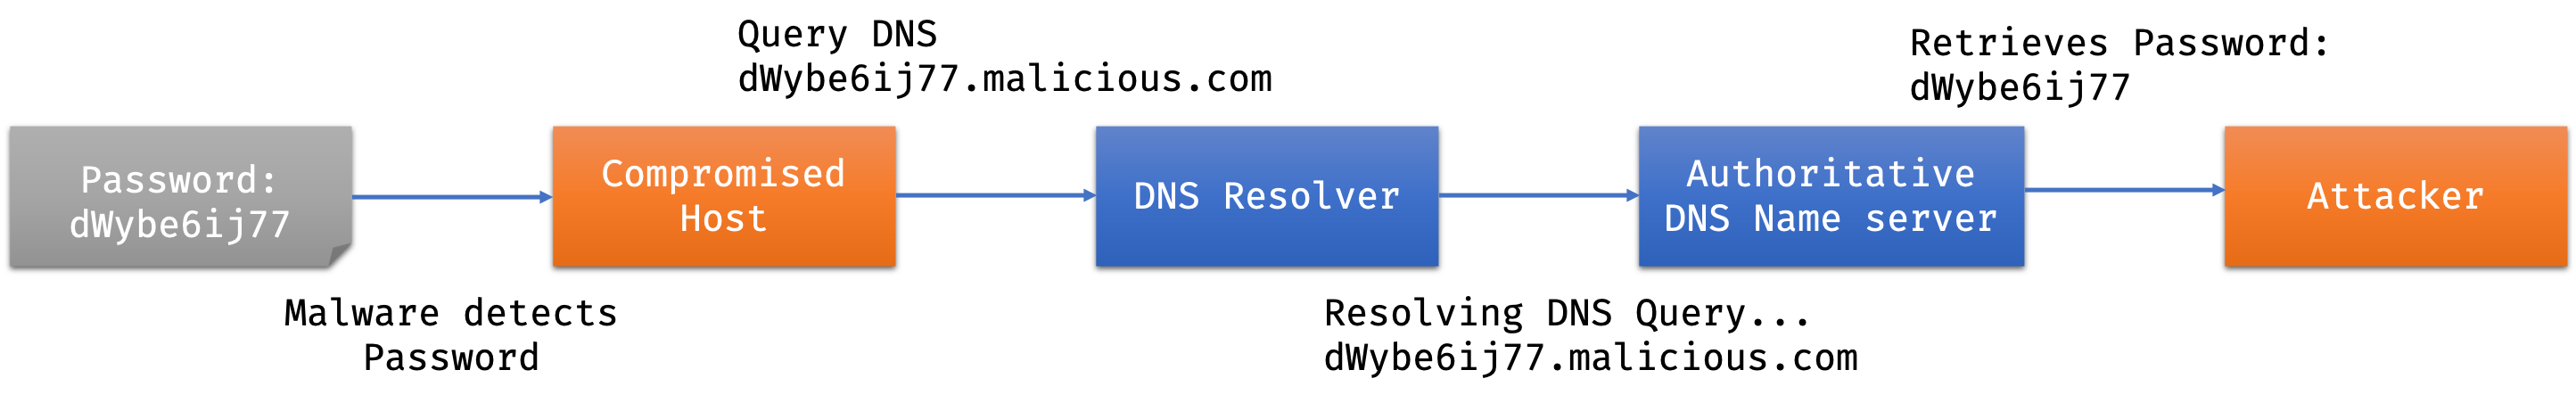
\includegraphics[width=\textwidth]{imgs/dns-data-exfil-out.png}
  \caption{Malware extracting password from host through DNS}
  \label{fig:dns-data-exfil-out}
\end{figure}

Similarly, Figure \ref{fig:dns-data-exfil-cycle} demonstrates an example where the malware queries C\&C for commands to achieve remote control on the compromised host. The DNS query remains similar to the example above in Figure \ref{fig:dns-data-exfil-out}; the difference lies in the DNS reply from the \url{malicious.com} name server. The attacker can respond with a Canonical Name (CNAME) record (or Text (TXT), Sender Policy Framework (SPF) record) indicating the instruction, usually with a very short TTL, so as to avoid this instruction being cached. The resolution of this DNS query on the compromised host would instruct the malware to act as ordered, in this particular figure, to read files and folders in \url{~/Documents}.

\begin{figure}[h!]
  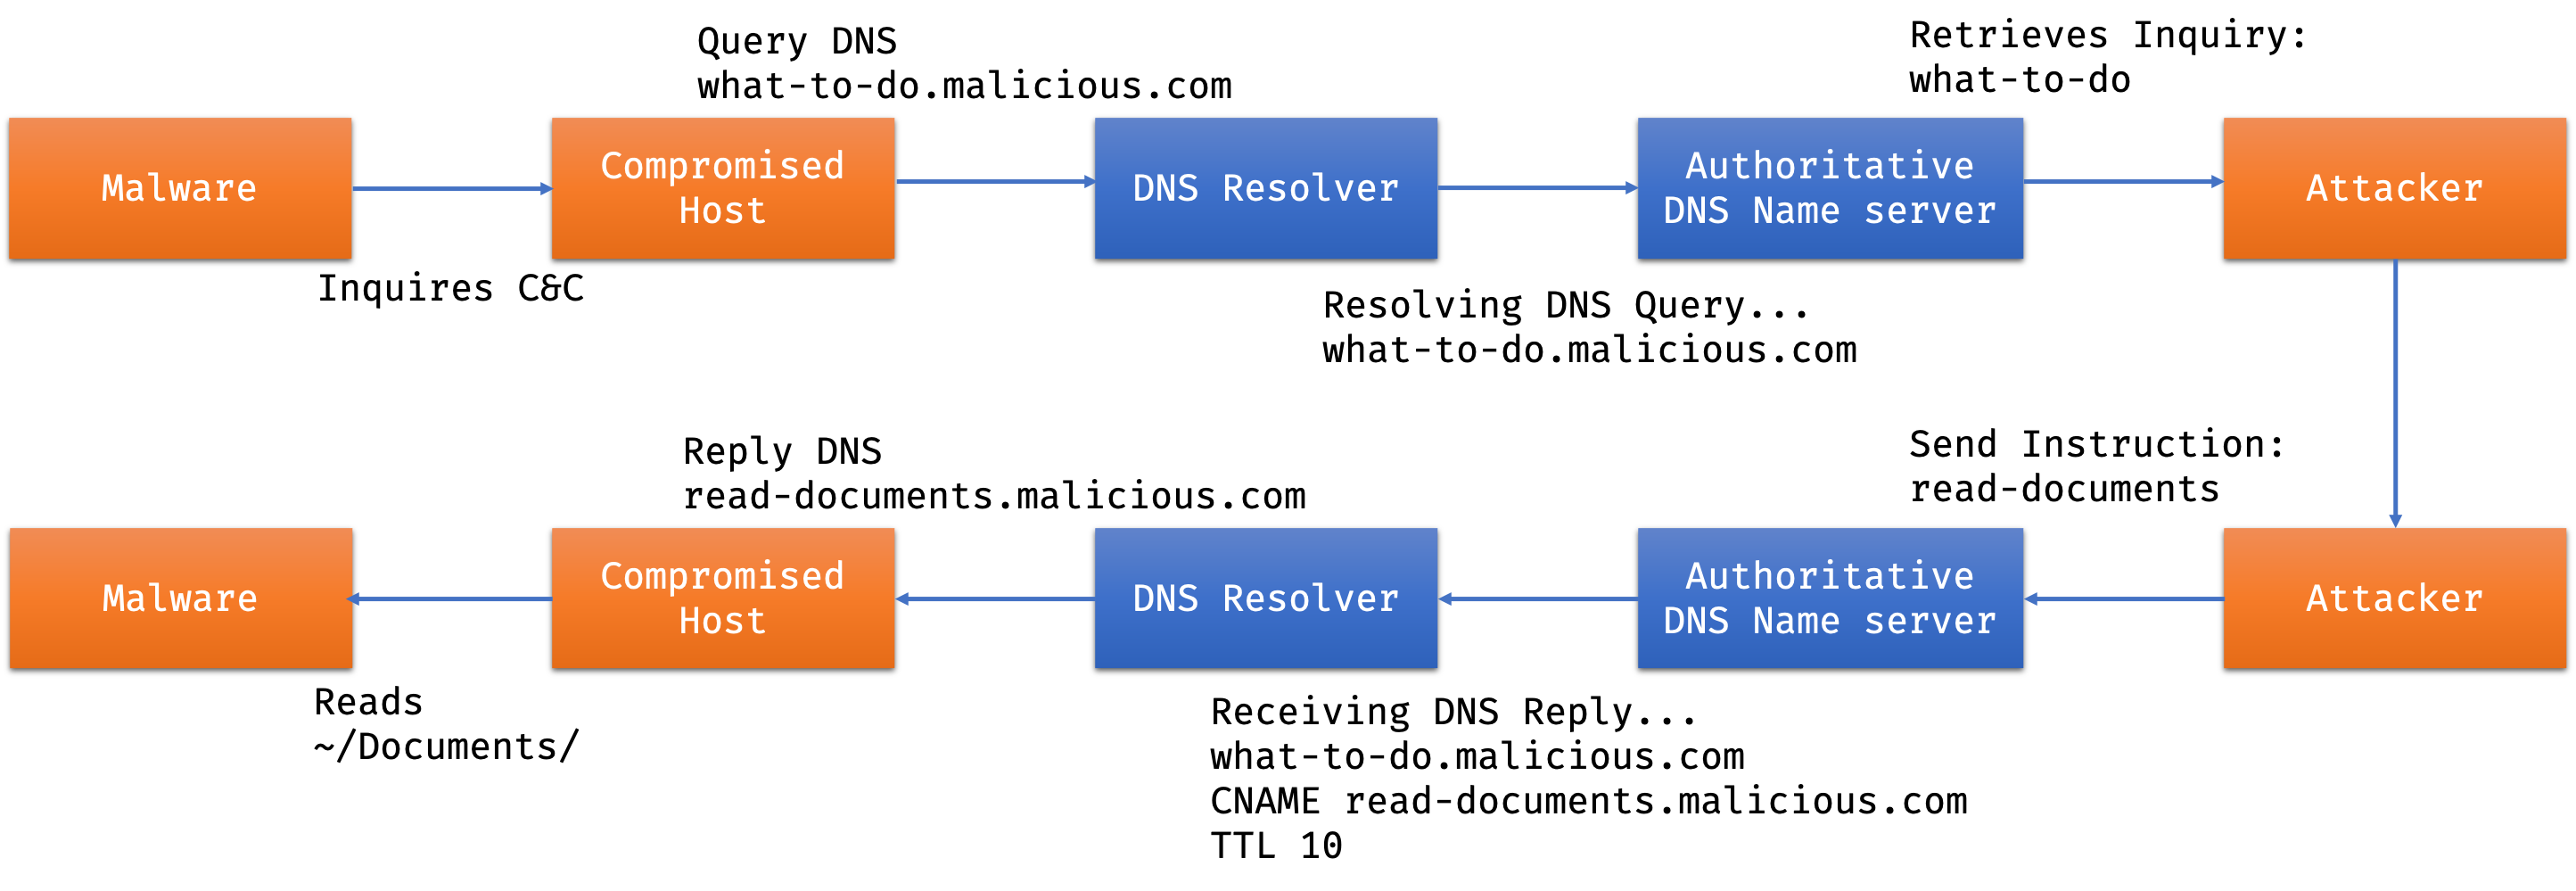
\includegraphics[width=\textwidth]{imgs/dns-data-exfil-cycle.png}
  \caption{Malware executing commands from remote C\&C}
  \label{fig:dns-data-exfil-cycle}
\end{figure}

Malware exploiting DNS for data exchanges can be divided into two major approaches: high-throughput tunnelling and low-throughput tunnelling.

As of high-throughput tunnelling, the malware would establish a bi-directional communication channel on top of the DNS via emulating a reliable and packet ordered network session between the compromised server and its C\&C. For example, the malware can enforce a Transmission Control Protocol (TCP) on top of DNS or send constant ping messages throughout communication to understand the replies' order. However, applying these methodologies would significantly increase the total amount of DNS traffic and each DNS packet's length while vastly decreasing the meantime between DNS transactions \cite{nadler-2017, nadler-201936}. As seen in Figure \ref{fig:dns-high-throughput-tunnelling}, the query intervals are less than 1 second due to the regular session keep-alive messages, the response towards the same queried domain \url{paaqfiiq.iodine.exfiltration.party} varies notably to signal a two-way communication tunnel, and some query length exceeds 200 bytes. These unusual characteristics compared to normal DNS traffic implies the existence of data exchange and exfiltration on top of DNS \cite{nadler-2017}.

\begin{figure}[h!]
  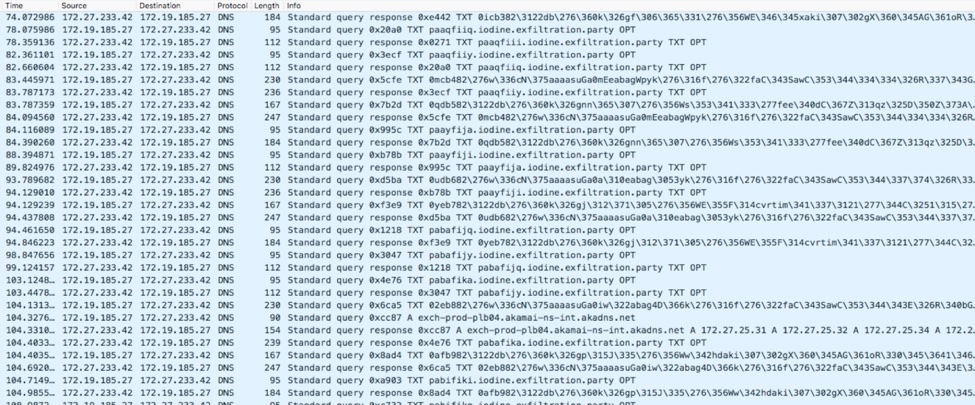
\includegraphics[width=\textwidth]{imgs/data-exfil-high-throughput-pcap.jpg}
  \caption{Sample \url{.pcap} file captured when running high-throughput DNS tunnelling}
  \label{fig:dns-high-throughput-tunnelling}
\end{figure}

Compared to high-throughput tunnelling, low-throughput tunnelling is generally harder to detect and remains overlooked within the cyber-security community \cite{nadler-2017, nadler-201936, ahmed-2020}.
To circumvent anomaly detection methods and firewalls, attackers would typically avoid using TCP tunnels or sending constant ping messages. Alternatively, the malware would wake up periodically, or triggered by specific activities, to deliver poll messages and a summary of machine activities to the C\&C \cite{nadler-2018}. For example, an infected Point-of-Sale (POS) terminal would be triggered upon a swipe and send transaction and card details to the attacker's C\&C without waiting for a response.

Detecting DNS tunnelling has been widely researched over the last decade, including detecting covert tunnelling \cite{gilbert-2009, davis-2016} and high-throughput DNS tunnelling \cite{wang-2016, buczak-2016, cambiaso-2016, engelstad-2017, homem-2017, kara-2014, sheridan-2015}. However, most publicly available detection solutions focus on high-throughput tunnelling due to its distinguishable network behaviour. These detection solutions rely heavily on the volume and variety of requests DNS tunnelling tools generate \cite{nadler-2017, nadler-2018}. One of the most popular solutions is DNS traffic rate control, offered by most security vendors \cite{homem-2017, nadler-2017}. More sophisticated solutions include supervised learning models on tunnelling DNS traffic, and non-tunnelling DNS traffic \cite{buczak-2016}, and anomaly detection models that would trigger upon notable change over DNS traffic as a whole \cite{davis-2016, sheridan-2015}. Yet, these algorithms are still distant from real-world applications with less ideal false-positive and false-negative rates.

\begin{table}[h]
\resizebox{\textwidth}{!}{%
\begin{tabular}{l|l|l|l}
Year & Malware       & Targets    & Malicious Domain Name   \\ \hline
2017 & DNS Messenger & Enterprise & \url{cspg.pw, algew.me}                          \\
2016 & MULTIGRAIN    & POS        & \url{dojfgj.com}                                 \\
2015 & BernhardPOS   & POS        & \url{29a.de}                                     \\
2015 & JAKU          & Botnet     & \url{LS4.com}                                    \\
2015 & Wekby         & Enterprise & \url{ns1.logitech-usa.com}                       \\
2014 & FrameworkPOS  & POS        & \url{a23-33-37-54-deploy.akamaitechnologies.com} \\
2014 & PlugX         & RDP/RAT    & \url{ns4.msftncsl.com}                           \\
2011 & FeederBot     & Botnet     & \url{images.moviedyear.net}                      \\
2011 & Morto         & RDP/RAT    & \url{ms.jifr.co.cc., ms.jifr.net.}      
\end{tabular}
}
\caption{A survery of malware from 2011-2018 exploiting DNS for low-throughput data exfiltration and exchange \cite{nadler-201936}}
\label{table:survey-malware-low-throughput-dns}
\end{table}

Although the topic of high-throughput DNS tunnelling has been studied thoroughly, little progress has been made on low-throughput DNS data exfiltration/exchange \cite{nadler-201936, steadman-2018, ahmed-2020}. A recent survey conducted by Nadler et al. \cite{nadler-201936} shown in Table \ref{table:survey-malware-low-throughput-dns} listed a number of malware exploiting DNS for low-throughput data exfiltration/exchange exposed in the period from 2011 to 2018. These malware targets vary from enterprise networks, botnets, POS terminals to Remote Desktop Protocol (RDP) / Remote Access Trojan (RAT). Meanwhile, the set of internet domains used by these malware includes concise ones (i.e. \url{29a.de}) to maximise the data exchange rate under the 255-byte query limit, and misleading ones (i.e. \url{ns1.logitech-usa.com}) imitating well-known brands to better hide under the human inspection of DNS traffic \cite{nadler-201936}. Detecting and blocking these low-throughput types malicious DNS traffic is much more difficult given its minimal proportion across the overall DNS traffic within an extensive network. Defending against these malware would require Deep Packet Inspection (DPI) from a Layer-7 firewall to at least parse through all DNS packets. This would induce extra latency to DNS transactions and slow down performance-critical services within the network. 

Hence, in this project, we will be targetting the construction of a solution that detects and blocks, upon request, both types of DNS data exfiltration/exchange methods reliably without introducing significant latency to the network.

\subsection{DNS Flood}
\label{section:background-dnsflood}

A DNS flood attack is a type of DDoS attack, as shown in Figure \ref{fig:dns-flood}, where malicious incoming traffic floods the victim's server, making it unable to provide normal service to legitimate users for a prolonged period \cite{cloudflare-dns-flood}. Given that DNS is the backbone service translating domain names to IPv4 addresses, successfully attacking DNS name servers can make a significant proportion of the Internet unusable for most people. Furthermore, in recent years, there has been a substantial rise in IoT devices, a considerable number of which are poorly secured \cite{mahjabin-2019}. In 2016, a botnet malware, Mirai\cite{bisson-2016}, utilised the high-bandwidth connections of IP cameras, Network Video Recorder (NVR) boxes and many other IoT devices to directly overwhelm name servers owned by DYN, a major DNS service provider. The peak flood bandwidth reached more than $12$ Gigabits per second, with more than $1$ million packets directed at a single DNS name server, resulting in significant take-downs of multiple popular websites, including GitHub, Netflix, Amazon, etc. \cite{bisson-2016, akamai-dns-flood}.

\begin{figure}[h!]
  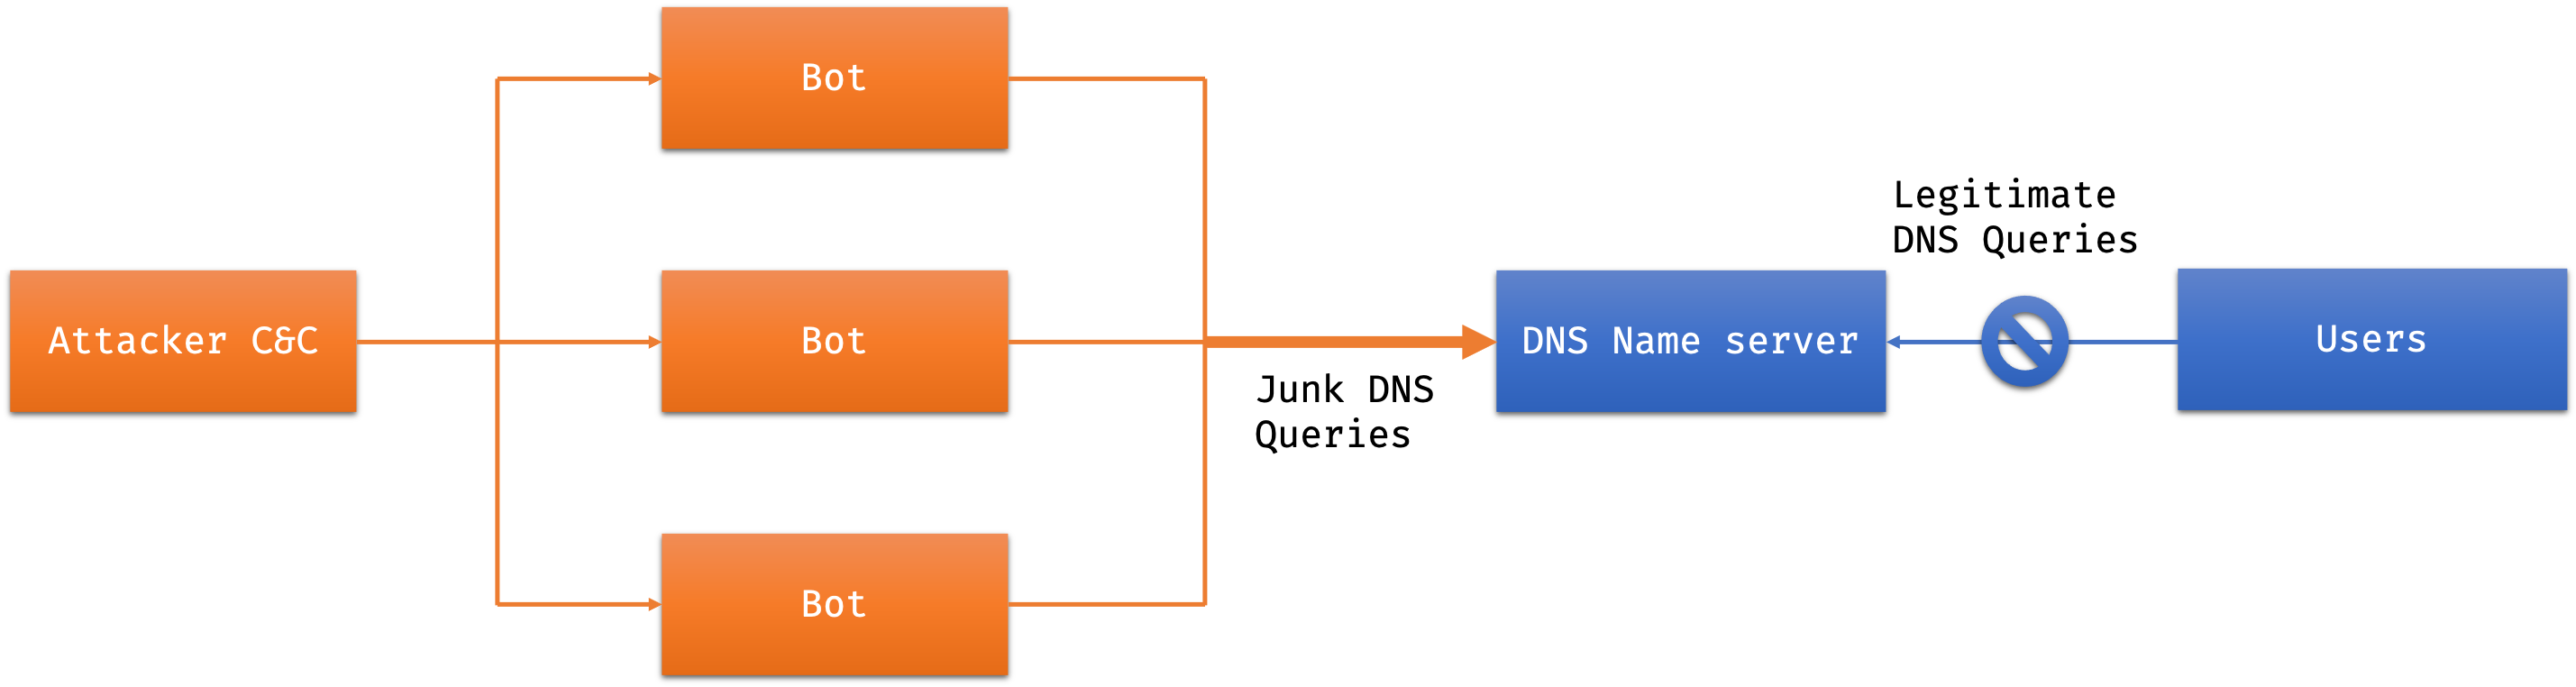
\includegraphics[width=\textwidth]{imgs/dns-flood.png}
  \caption{Botnet commencing DNS flood attack targetting a DNS name server}
  \label{fig:dns-flood}
\end{figure}

DNS flood attacks are designed to circumvent DNS resolvers' caching and continuously force DNS queries to go to certain authoritative name servers. This is done via a technique named Pseudo-Random Subdomain (PRSD) \cite{akamai-dns-flood}. The botnet attacker targetting a domain would generate a great number of non-existent prefixed subdomain requests, causing each bot's corresponding DNS resolver to continuously query the authoritative name server with a \code{NXDOMAIN} reply. In the cases where the bots that are conducting a DNS flood are making requests to name servers directly, blocking such clients and imposing a request rate limit could be straight forward. However, it is more likely that these malicious DNS queries are coming from upstream ISP DNS resolvers or public resolvers, which would not cache the \code{NXDOMAIN} reply to save resources \cite{akamai-dns-flood}. This complicates the DNS flood mitigation process as rate-limiting or blocking these public / ISP DNS resolvers risks throttling legitimate queries from users, which happen to share the same resolvers.

As a Cloudflare paper \cite{cloudflare-dns-flood} points out, a DNS flood attack represents a change from the traditional DNS amplification based attack methods. DNS flood is an application attack (Layer 7) rather than a volumetric attack (Layer 3). There is no spoofing required for DNS flood, nor does the request comes directly from the attacking source, but upstream DNS resolvers \cite{akamai-dns-flood, cloudflare-dns-flood}. Realistically, a NS flood would not be eliminated until most compromised IoT devices could be secured by updating firmware or replacing easy-to-guess passwords. Assuming the existence of a large and distributed DNS name server group, we attempt to tackle this problem by building a performant packet processing solution to absorb and block the attack traffic in real-time.

\subsection{Field Programmable Gate Arrays (FPGA)}
\label{section:background-fpga}

An FPGA is a type of integrated circuit designed to be customised by a designer after its fabrication, hence ``programmable on the field". As shown in Figure \ref{fig:fpga-arch}, it contains a matrix of Configurable Logic Blocks (CLBs) and higher levels of configurable interconnect, which activate and link the blocks in the manner the developer specifies \cite{xilinx-fpga}. There are two types of FPGAs, one-time programmable (OTP) devices and re-programmable devices \cite{xilinx-fpga}. Since OTP FPGAs are rare and outdated, we will mainly discuss Static Random Access Memory (SRAM) based re-programmable FPGAs.

\begin{figure}[h!]
  \centering
  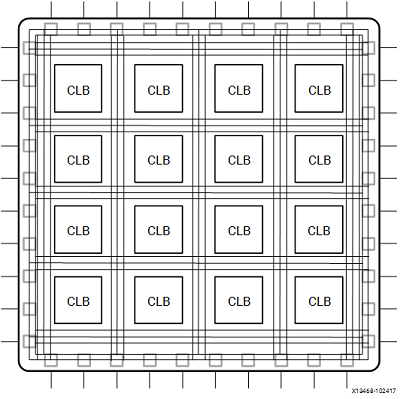
\includegraphics[width=0.3\textwidth]{imgs/fpga-arch.png}
  \caption{FPGA Architecture \cite{xilinx-fpga}}
  \label{fig:fpga-arch}
\end{figure}

Software network middlewares including firewalls \code{netfilter}/\code{iptables} \cite{netfilter-iptables}, \code{pf} \cite{pf}, \code{ipfw} \cite{ipfw} have been widely used in industrial and enterprise networks. As the network bandwidth grows, these software-based network middlewares are heavily limited by the parallelism and processing power of a single CPU. They can no longer meet the line rate packet processing requirements for large networks with high link speeds, typically $40$ Gbps and beyond \cite{fiessler-2016}. Therefore, we have seen an increasing number of packet processing systems built upon special purpose hardware, such as network processors (NPUs) \cite {qi-2007, duo-2006}, FPGAs\cite{hager-2014, fong-2012, jiang-2009, jiang-2009-large} and even ASICs \cite{bosshart-2013}. These hardware-based solutions provide an abundant amount of parallelism and can scale up almost linearly with minimal effort. Nowadays, the highest grade 7nm ASIC packet processors can achieve an overall network throughput of more than $25.6$ Tbps \cite{tomahawk-2021}, with a single packet latency lower than $400$ ps, orders of magnitude faster than any of the software-based packet processors.

There are various types of trade-offs among different implementations of network processors with regards to development time and cost, as well as flexibility and long-term adaptability. Among all three, ASIC-based Network Interface Cards (NICs) have the highest performance and power efficiency but suffer from a long development cycle, high development cost, and minimal flexibility after fabrication \cite{amara-2006, deierling-2018}. Conversely, CPU-based or System-on-Chip (SoC) NICs are easier to program and can be deployed for highly complex use cases, as the CPU provides general computation and the highest flexibility among all three \cite{deierling-2018}. FPGA-based NICs strike a balance between ASICs and SoCs by providing ``field-programmable" hardware. In other words, FPGAs would have performance similar to that of ASICs since they are both integrated circuits for application-specific purposes while maintaining the flexibility of being adaptable and upgradable after fabrication. Due to circuit limitations, the performance, energy efficiency and achievable timing frequency of FPGAs is inferior to that of ASICs. On the other hand, FPGAs are much more complex to program than SoCs due to hardware timing constraints and electrical uncertainties, and a deployed FPGA algorithm would ultimately be limited by the number of logic units on the FPGA chip \cite{deierling-2018}.

\subsection{SipHash}
\label{section:background-siphash}

SipHash is an Add-Rotate-Xor (ARX) family of pseudo-random hash functions created in 2012 \cite{aumasson-bernstein-2012}, originally aimed at mitigating various ``hash-flooding" DDoS attacks seen in late 2011 \cite{lennon-2011}. SipHash has typically used as a Message Authentication Code (MAC) calculation method to guarantee the sender's authority and message's integrity. 

Let $X$ be a message string, and $k$ be a key string, SipHash guarantees that, even if an attacker has seen $X$ and $\code{SipHash}(X, k)$, an attacker who does not know $k$ would not be able to find out $k$ nor construct $\code{SipHash}(Y, k)$ for any message $Y \neq X$ that they have not seen before. Further cryptanalysis and mathematical proof of the promise above have been done by Christoph et al. \cite{dobraunig-2014} and Xin et al. \cite{xin-2019}.

SipHash has several unique characteristics that make it a suitable candidate for hardware implementation, namely simplicity, simple middle states, and minimal overhead \cite{aumasson-bernstein-2012}. The algorithm iterates a simple SipRound function utilised multiple times; hence the hardware component and circuit can be reused at different clock cycles. Siphash's middle states consists of only four 64-bit variables $v_0 ... v_4$. From a hardware implementation perspective, it minimises Flip-Flop (FF) usages, easing the design implementation on the board. Most importantly, the generated MAC is concise and of designated length (64 bits), bringing minimal and fixed consumption of hardware units.

\section{Related Work}

Although FPGAs have been used to build various network appliances, very little public research has considered using an FPGA against DNS exfiltration attacks. Thomas et al. \cite{thomas-2011} proposed an FPGA-based system for detecting malicious DNS network traffic, which only extracts DNS query domains and matches them by hash against a list of hard-coded domain names within the memory. This approach is limited by the lack of real-time adaptability of the filter list and the inability to mitigate DNS exfiltration and flood attacks on the fly. 

With regards to using FPGAs to mitigate DNS flood attacks, most related research aims at mitigating DDoS attacks as a whole instead of DNS flood attacks in particular \cite{hoque-2017, nagy-2018, tokusashi-2016, thinh-2016}. FPGAs have been used to detect DDoS attacks in real-time \cite{hoque-2017} and mitigate such attacks with very low reaction time \cite{nagy-2018}. However, most research aimed at mitigating DDoS attacks using FPGAs focused primarily on DNS Amplification attacks \cite{nagy-2018, thinh-2016, tokusashi-2016}, as these were more prevalent and could be used to target individuals or smaller networks with poor protection in place. With reference to Section \ref{section:background-dnsflood}, the Mirai botnet's successful DNS flood attack against major DNS providers proves the inability of traditional mitigation methods against these new types of Layer 7 DDoS attacks. 

\section{Project Motivation}

This project introduces an FPGA-based solution that tackles two major rising threats exploiting the DNS protocol, DNS exfiltration attacks and DNS flood attacks. We will be improving on the FPGA DNS filter from Thomas et al. \cite{thomas-2011} by bringing real-time reconfigurability to our FPGA-based system. Innovatively, we will be further providing instantaneous	mitigation against DNS exfiltration transactions via hardware-accelerated DNS spoofing. Meanwhile, legitimate DNS transactions can proceed safely with minimal overhead.

Moreover, since most FPGA logic can be reused, namely traffic filtering and packet parsing in the aforementioned system, we further develop a separate FPGA operation mode to act as a low-latency Layer 7 firewall, mitigating DNS flood attacks.

As the system will be used in high-bandwidth and latency-sensitive environments, we deem it necessary to develop an application-specific hardware solution for this task. Given the analysis in Section \ref{section:background-fpga} of ASIC and FPGA network processors, we preferred the FPGA in our project implementation due to the cost and time limitations of a single-person final-year project.


\chapter{Design}

In this chapter, we will be presenting both the internal system design of the solution and the overall network design that this system will put into practice. We will be elaborating on the design thought process and several design choices and considerations we made for the computing hardware and software control system. Also, we will be discussing some example topologies to illustrate how the solution will work to secure the network.

\section{System Design}

\subsection{Hardware Design}
\label{section:design-system-design-hardware}

\begin{figure}[h!]
  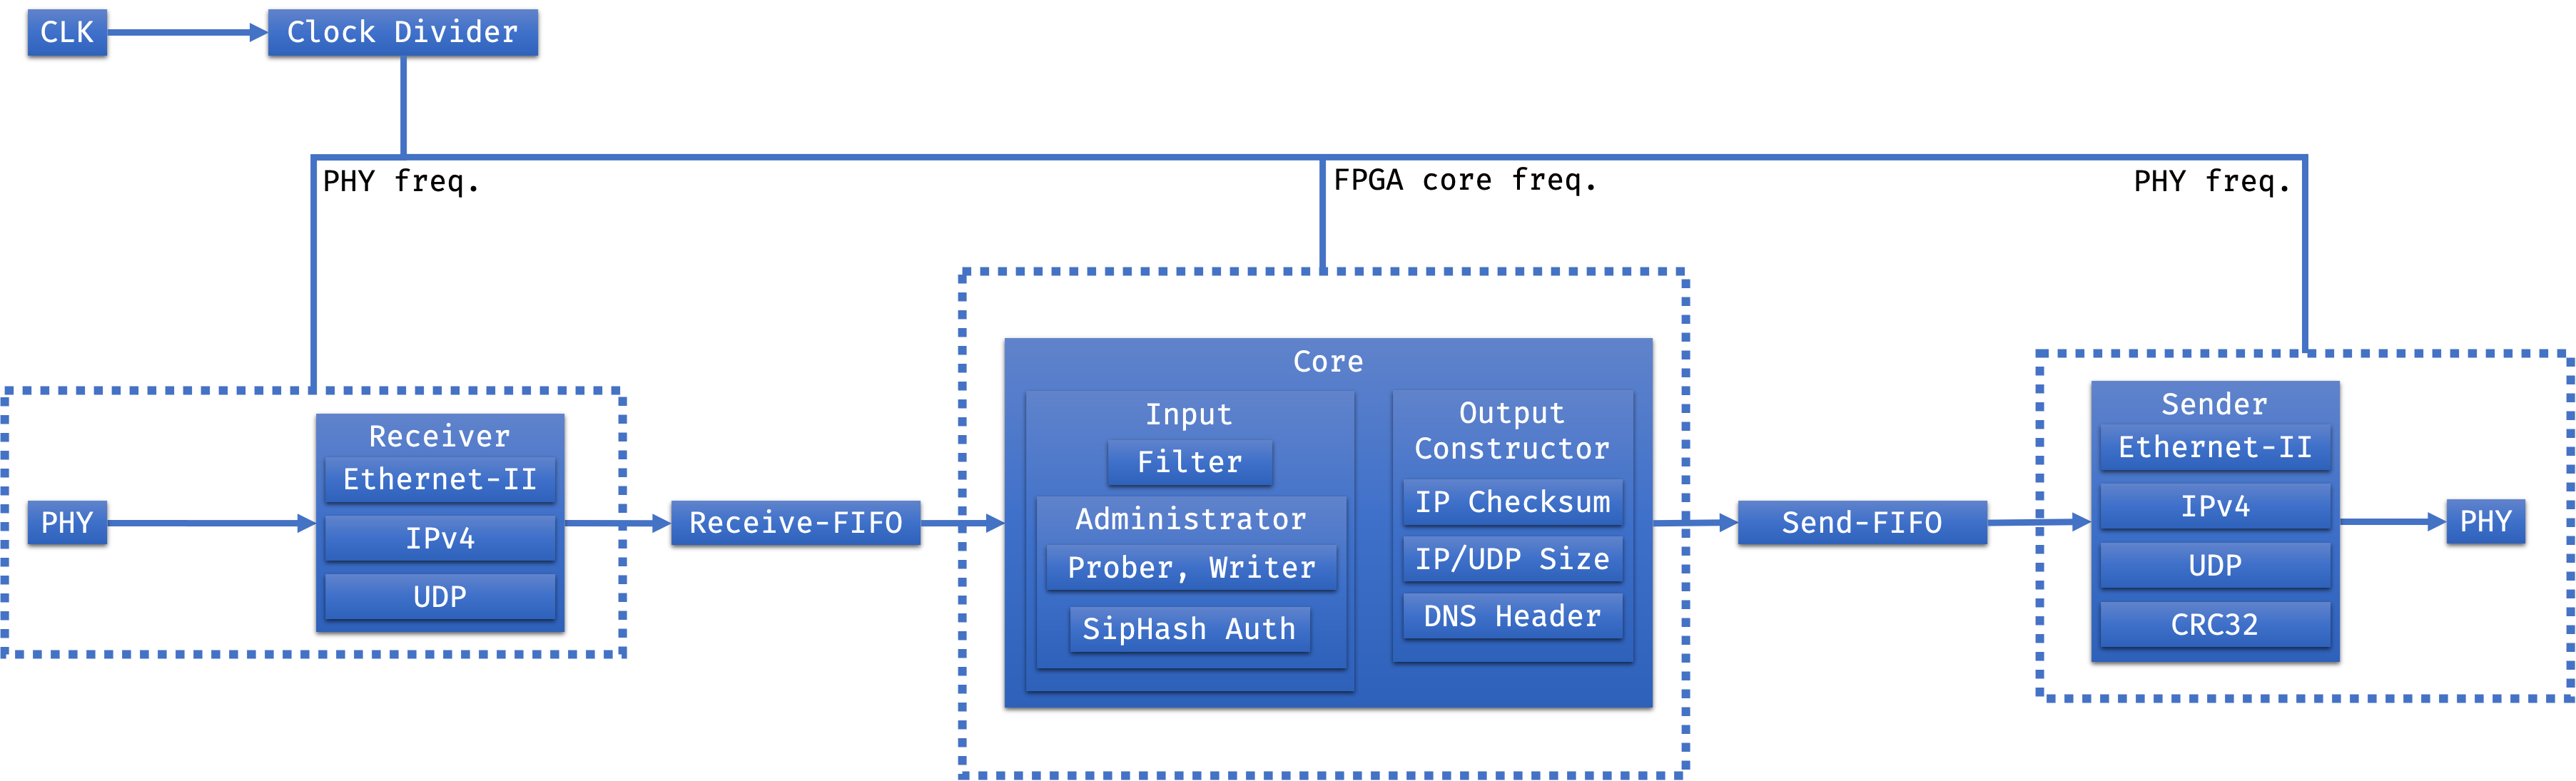
\includegraphics[width=\textwidth]{imgs/hardware-design.png}
  \caption{Hardware Architectural Design}
  \label{fig:hardware-design}
\end{figure}

Since we are designing a network processing circuit, we must be aware of the hardware interface we are interacting with. With an Ethernet-II PHY ASIC available on most development boards with RJ45 connectors, we assumed that our design would retrieve incoming bits from a specific type of Media-Independent Interface (MII) family\footnote{See Section \ref{section:implementation-hardware-implementation} for introduction to MII family and implementation details} \cite{ieee802.3ethernet-2018}. Similarly, we will be outputting bits to an MII-type interface as well at the end of processing. Hence, we can derive an initial architecture of a core processing component receiving from an input circuit and sending to an output circuit, as shown in Figure \ref{fig:hardware-design}.

Retrospectively speaking, the issue of assigning clock domains was not thought through carefully at the design stags and later became a pitfall that cost a significant amount of effort on regression and fixing. It is worth considering each component's clock domain and several clock domain crossing methods when designing the system. Generally, PHY ASIC chips operate at a lower clock frequency than the FPGA core, resulting in different clock domains within the system. The initial clock signal from the FPGA's clock path is designed to go through a clock divider that generates suitable clock signals for each component in various domains. Inevitably throughout the design, there would be signals crossing clock domains (i.e. from receiver to core module). If left unsynchronised, the destination domain would experience various meta-stability issues\footnote{See Section \ref{section:implementation-hardware-debugging} for more information on Clock Domain Crossing (CDC) and signal metastability in hardware}. Thus we introduce two asynchronous First-In-First-Out (FIFO) buffers that connect the receiver to the core and the core to sender, as shown between the clock regions in Figure \ref{fig:hardware-design}.

Within the Receiver and Sender components shown on the left and right side of Figure \ref{fig:hardware-design}, we aim to design a sequential circuit that utilises a Finite State Machine (FSM) that is mainly comprised of three parsing/packing stages, Ethernet-II, IPv4 and UDP. The sender ideally shall have an extra Ethernet Cyclic Redundancy Check 32-bit (CRC32) \cite{ieee802.3ethernet-2018} generation module that appends a 32-bit checksum to the packet. As for the core processing module, we aim to split it into two sub-components, one handling DNS parsing, Layer 7 filtering, FPGA administration and security checks, while the other is working on constructing proper DNS / payload responses and calculating sizes and checksums for higher-layer protocols (IPv4, UDP and DNS), as demonstrated in the Core section of Figure \ref{fig:hardware-design}.

\begin{figure}[h!]
  \makebox[\textwidth][c]{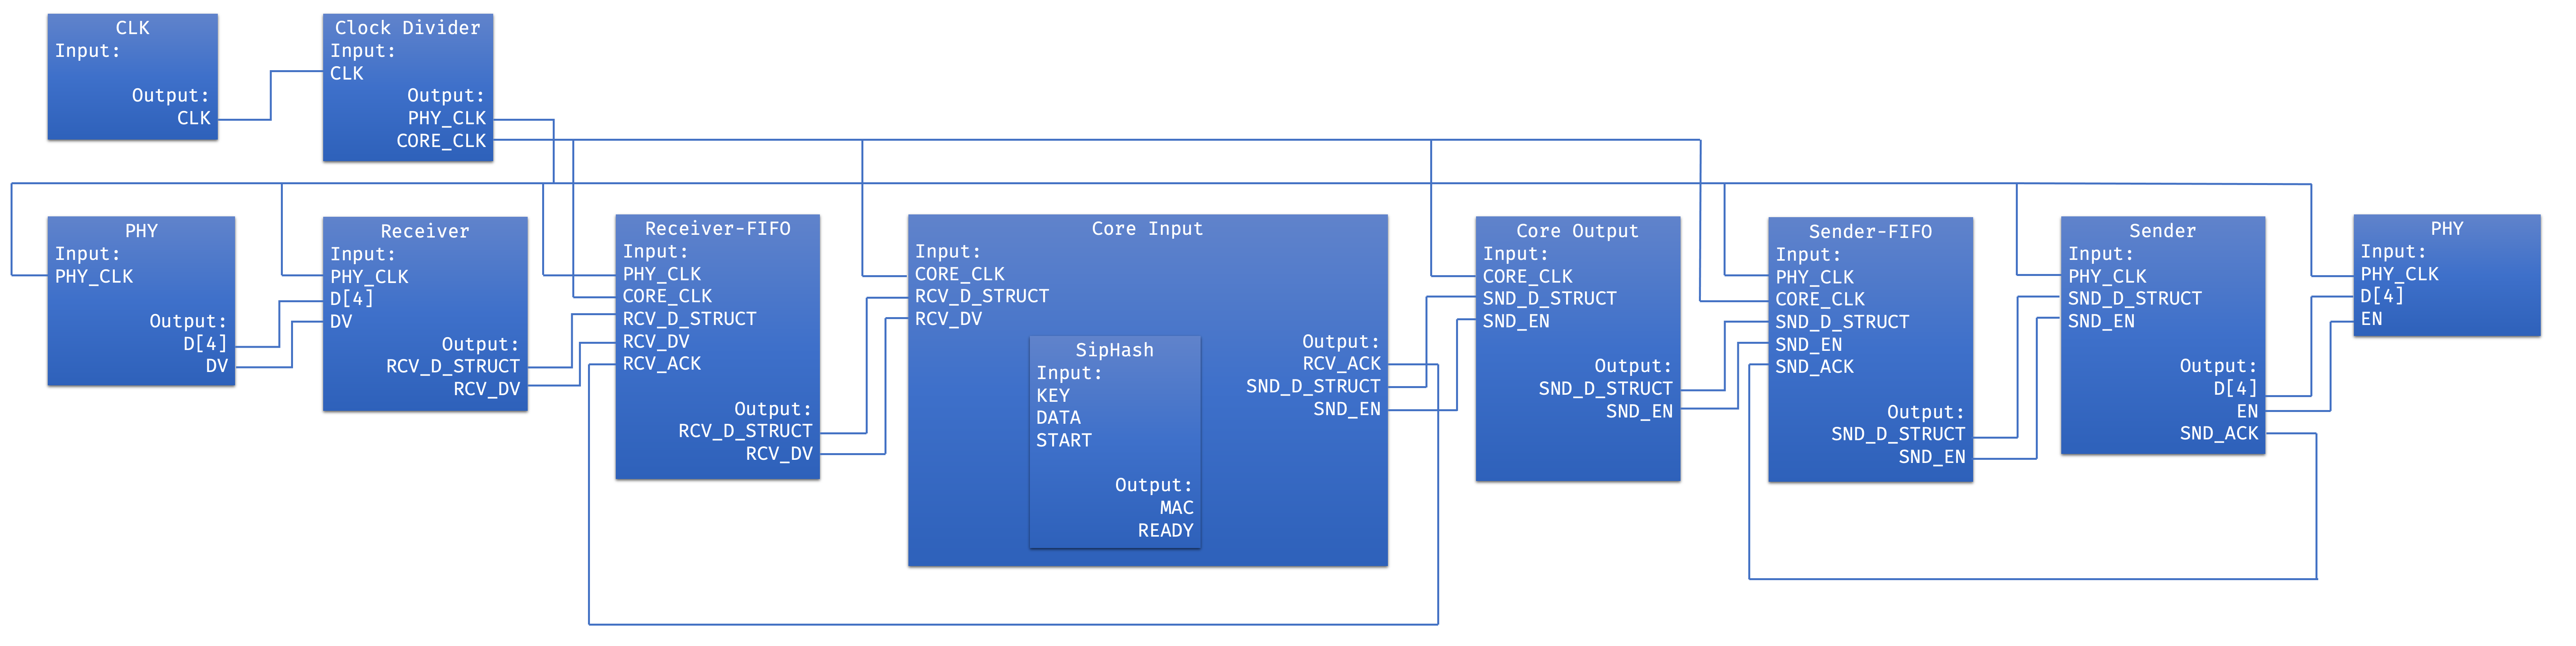
\includegraphics[width=1.1\textwidth]{imgs/hardware-signal.png}}
  \caption{Hardware Signal Design}
  \label{fig:hardware-signal-design}
\end{figure}

After designing the top-level components and their main functionalities, we sketch the signal schematic of the design so as to determine each component's incoming and outgoing ports, as laid out in Figure \ref{fig:hardware-signal-design}. The standard input for almost all synchronous sequential logic is the clock pin (\code{CLK}). As suggested previously in this section, components within different clock domains receive \code{CLK} at their corresponding frequencies. The only exception here is the cross-domain asynchronous FIFOs which need to be activated by \textit{both} \code{CLK} signals, one for writing to the FIFO queue and the other for reading.

To avoid actively reading and writing data when not required, we utilised various Data Valid (DV), Enable (EN) and ACKnowledgement (ACK) signals in our components, as seen in Figure \ref{fig:hardware-signal-design}. Each sequential component in hardware is designed to constantly check against a set of signals when in an idle state. The hardware designer specifies such set of signals as the sensitivity list of a \proglang{VHDL}'s process or a \proglang{Verilog}'s always-block. When the activation signal reaches Voltage Common Collector (VCC) level upon a rising clock edge, the sequential component transits into a working state and starts reading and processing the bits from other incoming signals. For example, in the core input (\code{corein}) module (Figure \ref{fig:hardware-signal-design}), we utilise two sensitive signals, \code{CLK} and \code{RCV\_DV} to ensure the data processing starts when both are at VCC level. The receiving data will then be read and further processed at later rising clock edges.

Besides clocking and activation signals, we also need to design data transfer ports across signals. We define a custom data structure \code{D\_STRUCT} to maintain all signals we need for processing and discard the rest of the unneeded packet information. The \code{D\_STRUCT} is an internal representation of the packet with relevant metadata and parsed DNS payload. This design allows us to keep a fixed-length representation of variable length packets within the hardware system\footnote{See Section \ref{section:implementation-hardware-debugging} for issues with the variable-length descriptors in hardware}. Moreover, we made every effort to keep the \code{D\_STRUCT} small in bit size so as to avoid using unnecessary FIFOs delaying data transfers or wasting FPGA resources. The trade-off in this approach is a lack of support for payloads longer than a pre-determined limit (128 bytes in our implementation\footnote{See Section \ref{section:implementation-hardware-implementation} for our detailed implementation of packet segmentation and the 128-byte limit}); however we think it is worthwhile to proceed with this approach as we focus primarily on processing typically shorter DNS packets with minimal latency.

\subsection{Software Design}

\begin{figure}[h!]
  \makebox[\textwidth][c]{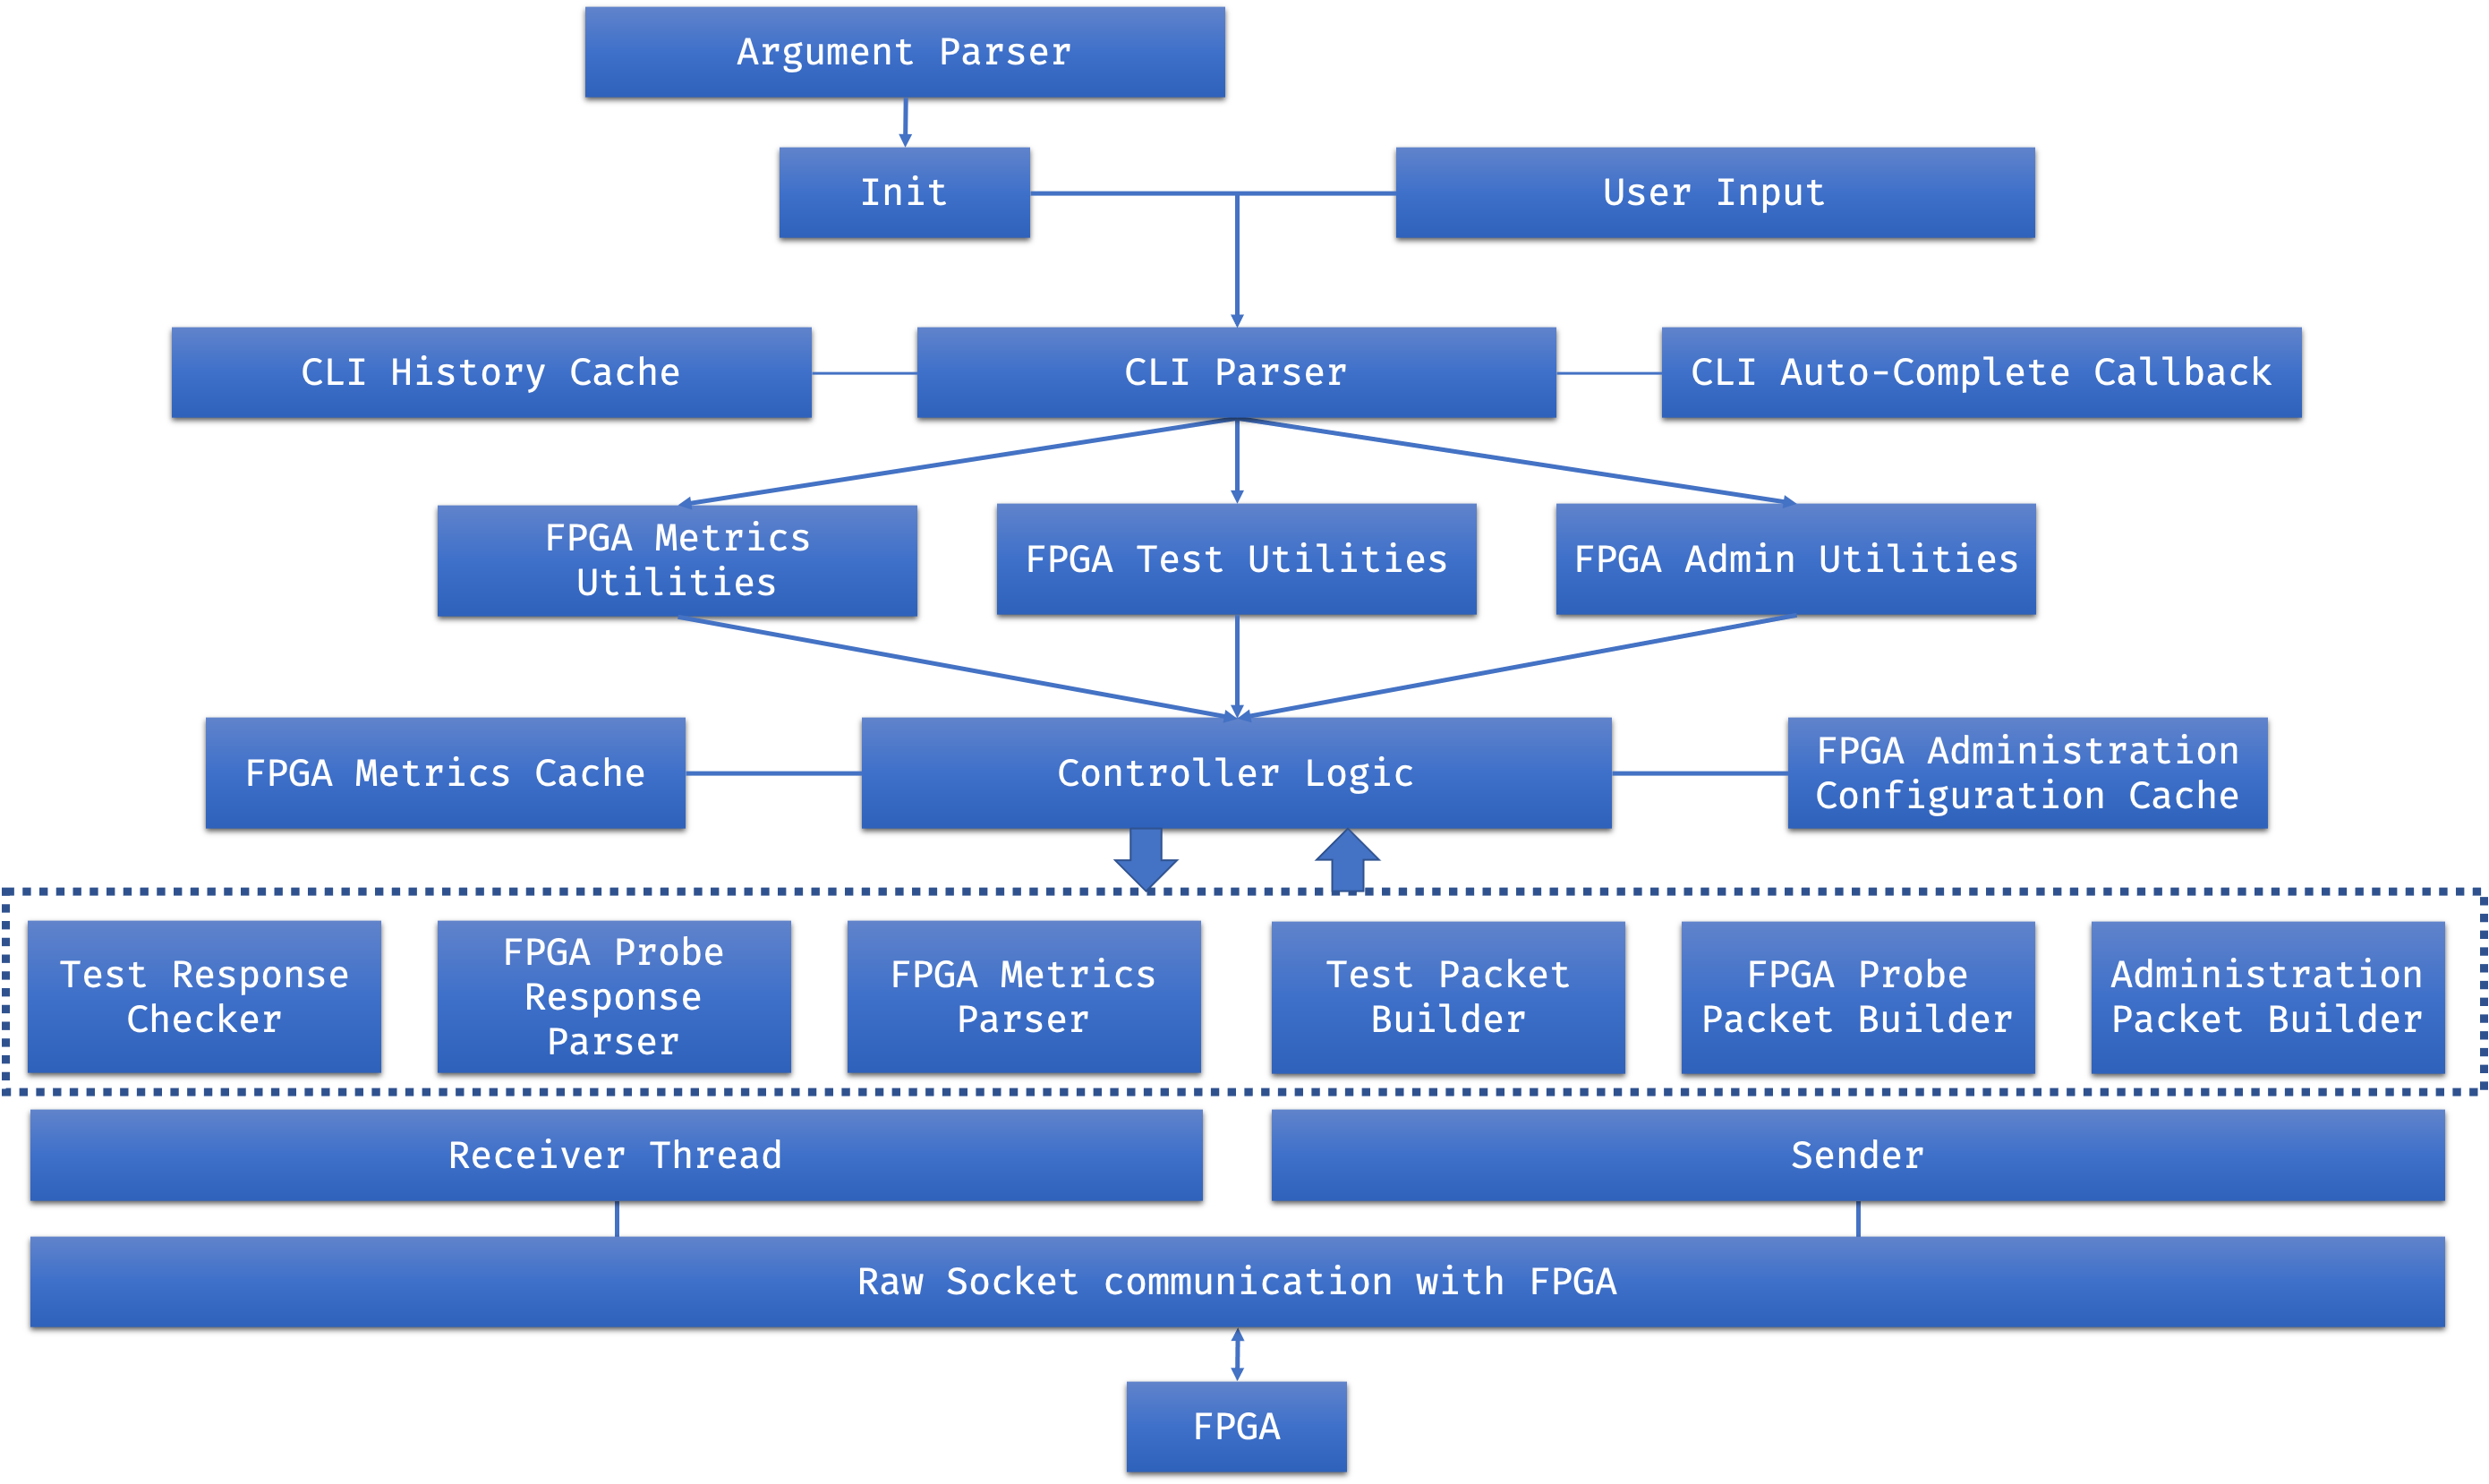
\includegraphics[width=1.1\textwidth]{imgs/software-design.png}}
  \caption{Software Design}
  \label{fig:software-design}
\end{figure}

As part of our goal to develop a resilient system, we also designed administrative software to control, monitor and reconfigure the FPGA in real-time. As with most network configuration software, we provide a Command Line Interface (CLI) front end to administrators. In the top layers of Figure \ref{fig:software-design}, the software front-end are comprised of an argument parser that understands launch options, a CLI parser that splits commands into function calls and their corresponding argument string, and several supporting features, namely CLI history and CLI auto-complete functionalities.

The software is designed to provide three main command families, \code{stats}, \code{test} and \code{admin}, corresponding to the three utilities in the middle layer of Figure \ref{fig:software-design}. 
\begin{itemize}
    \item \code{stats} commands provide the user with the ability to understand the accumulated statistics and metrics on the FPGA filter, including packets received, DNS replies sent, etc.
    \item \code{test} commands enable the user to test the hardware implementation of the FPGA system with integration tests and stress tests. This is to make sure the system on FPGA is functioning as expected and within the performance threshold.
    \item \code{admin} commands allow the user to read and write DNS filter and operation mode configurations on the FPGA. It also provides convenient features for admins to save and load FPGA admin configurations as files on the controlling system.
\end{itemize}

Since certain commands such as \code{admin show curr} (which shows the currently editing admin configuration) do not need direct information exchange with the FPGA, we utilise a central controller logic to determine back-end operations and avoid unnecessary probes of the FPGA. Therefore, as shown in the bottom layers of Figure \ref{fig:software-design}, we provide various packaged functions that interface with the FPGA for the controller to interact with. These functions are mainly divided into senders and receivers, which rely on two different raw sockets.

The receiver socket operates like a daemon thread listening to all network traffic on the FPGA interface. Noteworthy replies and metrics from the FPGA will be highlighted and saved to cache automatically upon capture. Then, relevant parsers or checkers will be called to verify or understand FPGA messages accordingly. 

The sender socket, on the other side of the spectrum, is only called when necessary. When the controller logic issues a command, the corresponding packet builder will build an administrative, test or probe packet that will be sent to the FPGA. A response might later be received and then coordinated by the receiver, as discussed above.

With the aim to provide a future proof system, we also designed APIs for more complex algorithms such as entropy-based anomaly detectors to fetch and analyse the metrics captured by the FPGA. After the analysis, the algorithms can proactively reconfigure the FPGA with several simple function calls. The APIs are designed as an extension, enabling developers to engineer complex algorithms making more intelligent decisions and push operational changes to FPGA instantaneously.

\section{System Usage Sample Topology}
\label{section:design-system-usage-sample}

\subsection{DNS Data Exfiltration}

The main innovative application of the FPGA-based system is to detect and mitigate DNS exfiltration attacks in real-time. Typically, the system would be deployed in a secure enterprise network with confidential information on its hosts (i.e. a cloud-based POS network, a military network with restricted Internet access). We assume that the network is originally set up with a firewall comprised of ASIC-based Layer 3/4 firewall and software-based Layer 7 firewall, bridging the connection between Wide Area Network (WAN) and the internal network switches. The FPGA shall connect to the network in a man-on-the-side manner with its operation mode set to ``Man-on-the-Side DNS spoofing".  In this particular configuration, as an example, the FPGA checkers are set to:

\begin{itemize}
    \item MAC checkers: Disabled
    \item IP checkers: Check against a known list of internal DNS server IPs
    \item UDP Port checkers: Check for port 53
    \item DNS checkers: Check for \url{enterprise.local} and \url{essential.service}
\end{itemize}

If a DNS transaction satisfies all checker requirements, the packet would then be deemed legitimate and passed on to its intended recipients. If not, the FPGA would send out a Spoofed \code{NXDOMAIN} reply (or any administrator configured DNS \code{RCODE} reply) to the host.

We can further configure the ASIC-based Layer 3 firewall or use a Network Test Access Point (TAP) device with the FPGA filter to achieve the following:

\begin{itemize}
    \item When sending a DNS packet to WAN:
        \SubItem    {If it is not sent from the FPGA, redirect it to the FPGA}
        \SubItem    {If it is sent from the FPGA, send to WAN}
    \item When receiving a DNS packet from WAN
        \SubItem    {Redirect it to the FPGA}
\end{itemize}


\begin{figure}[H]
  \makebox[\textwidth][c]{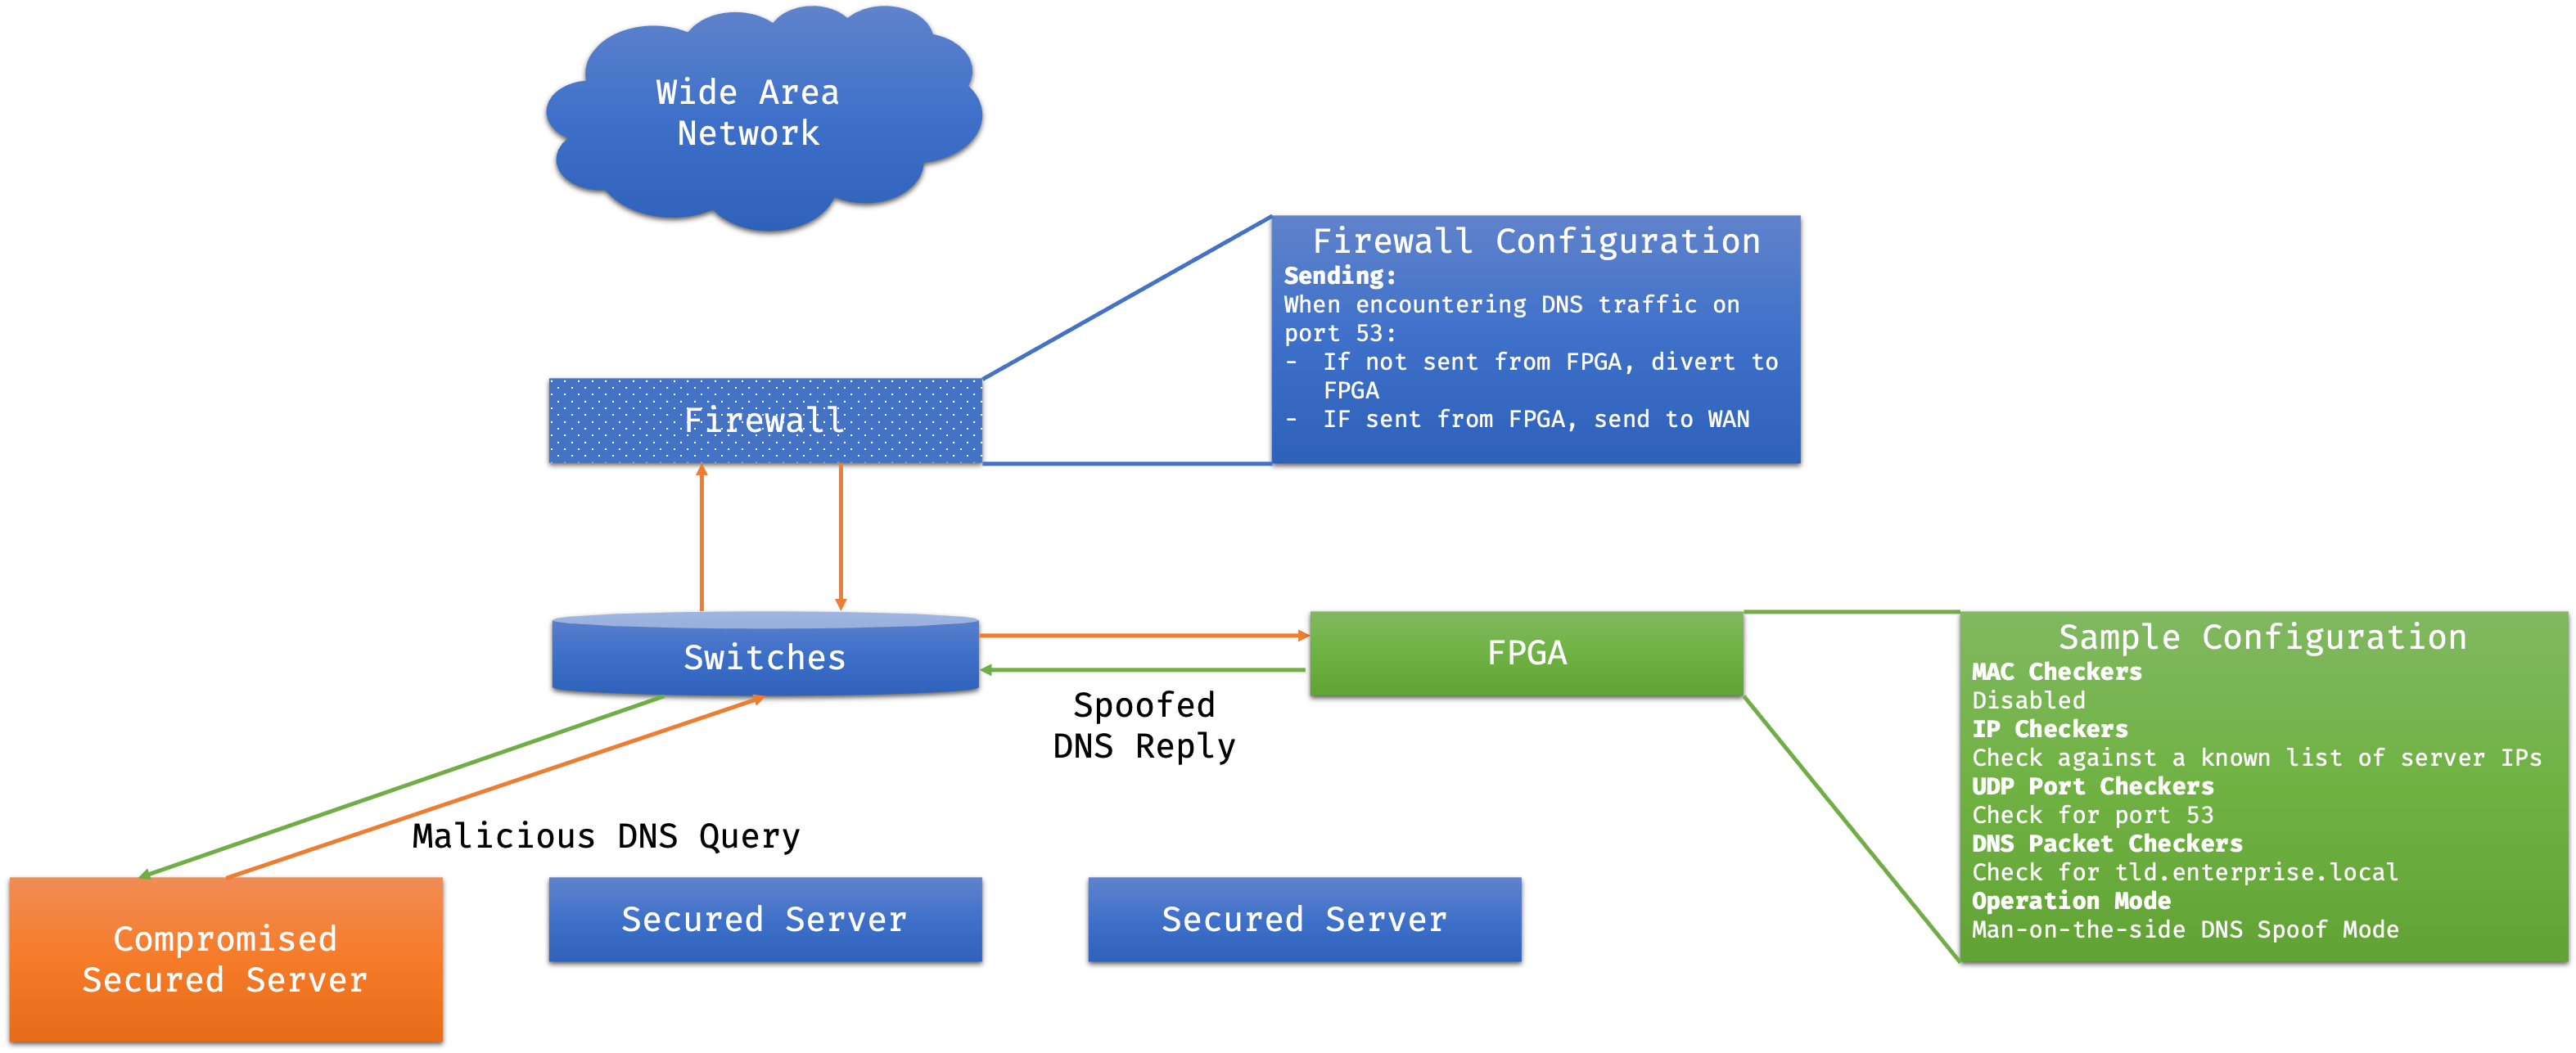
\includegraphics[width=1.1\textwidth]{imgs/man-on-the-side-malicious-dns-query.png}}
  \caption{Man-on-the-Side FPGA sample topology - Sending malicious DNS exfiltration / tunnelling query}
  \label{fig:man-on-the-side-FPGA-send-malicious}
\end{figure}

Generally, the initiative of data exfiltration usually starts from a compromised host within the network. In the event where the host sends a malicious DNS query exfiltrating data / establishing a tunnel in Figure \ref{fig:man-on-the-side-FPGA-send-malicious}, the firewall would first redirect the query to the FPGA. The FPGA would spot this DNS query as suspicious and send a spoofed DNS reply back to the compromised host, stopping the data exfiltration. 

\begin{figure}[H]
  \makebox[\textwidth][c]{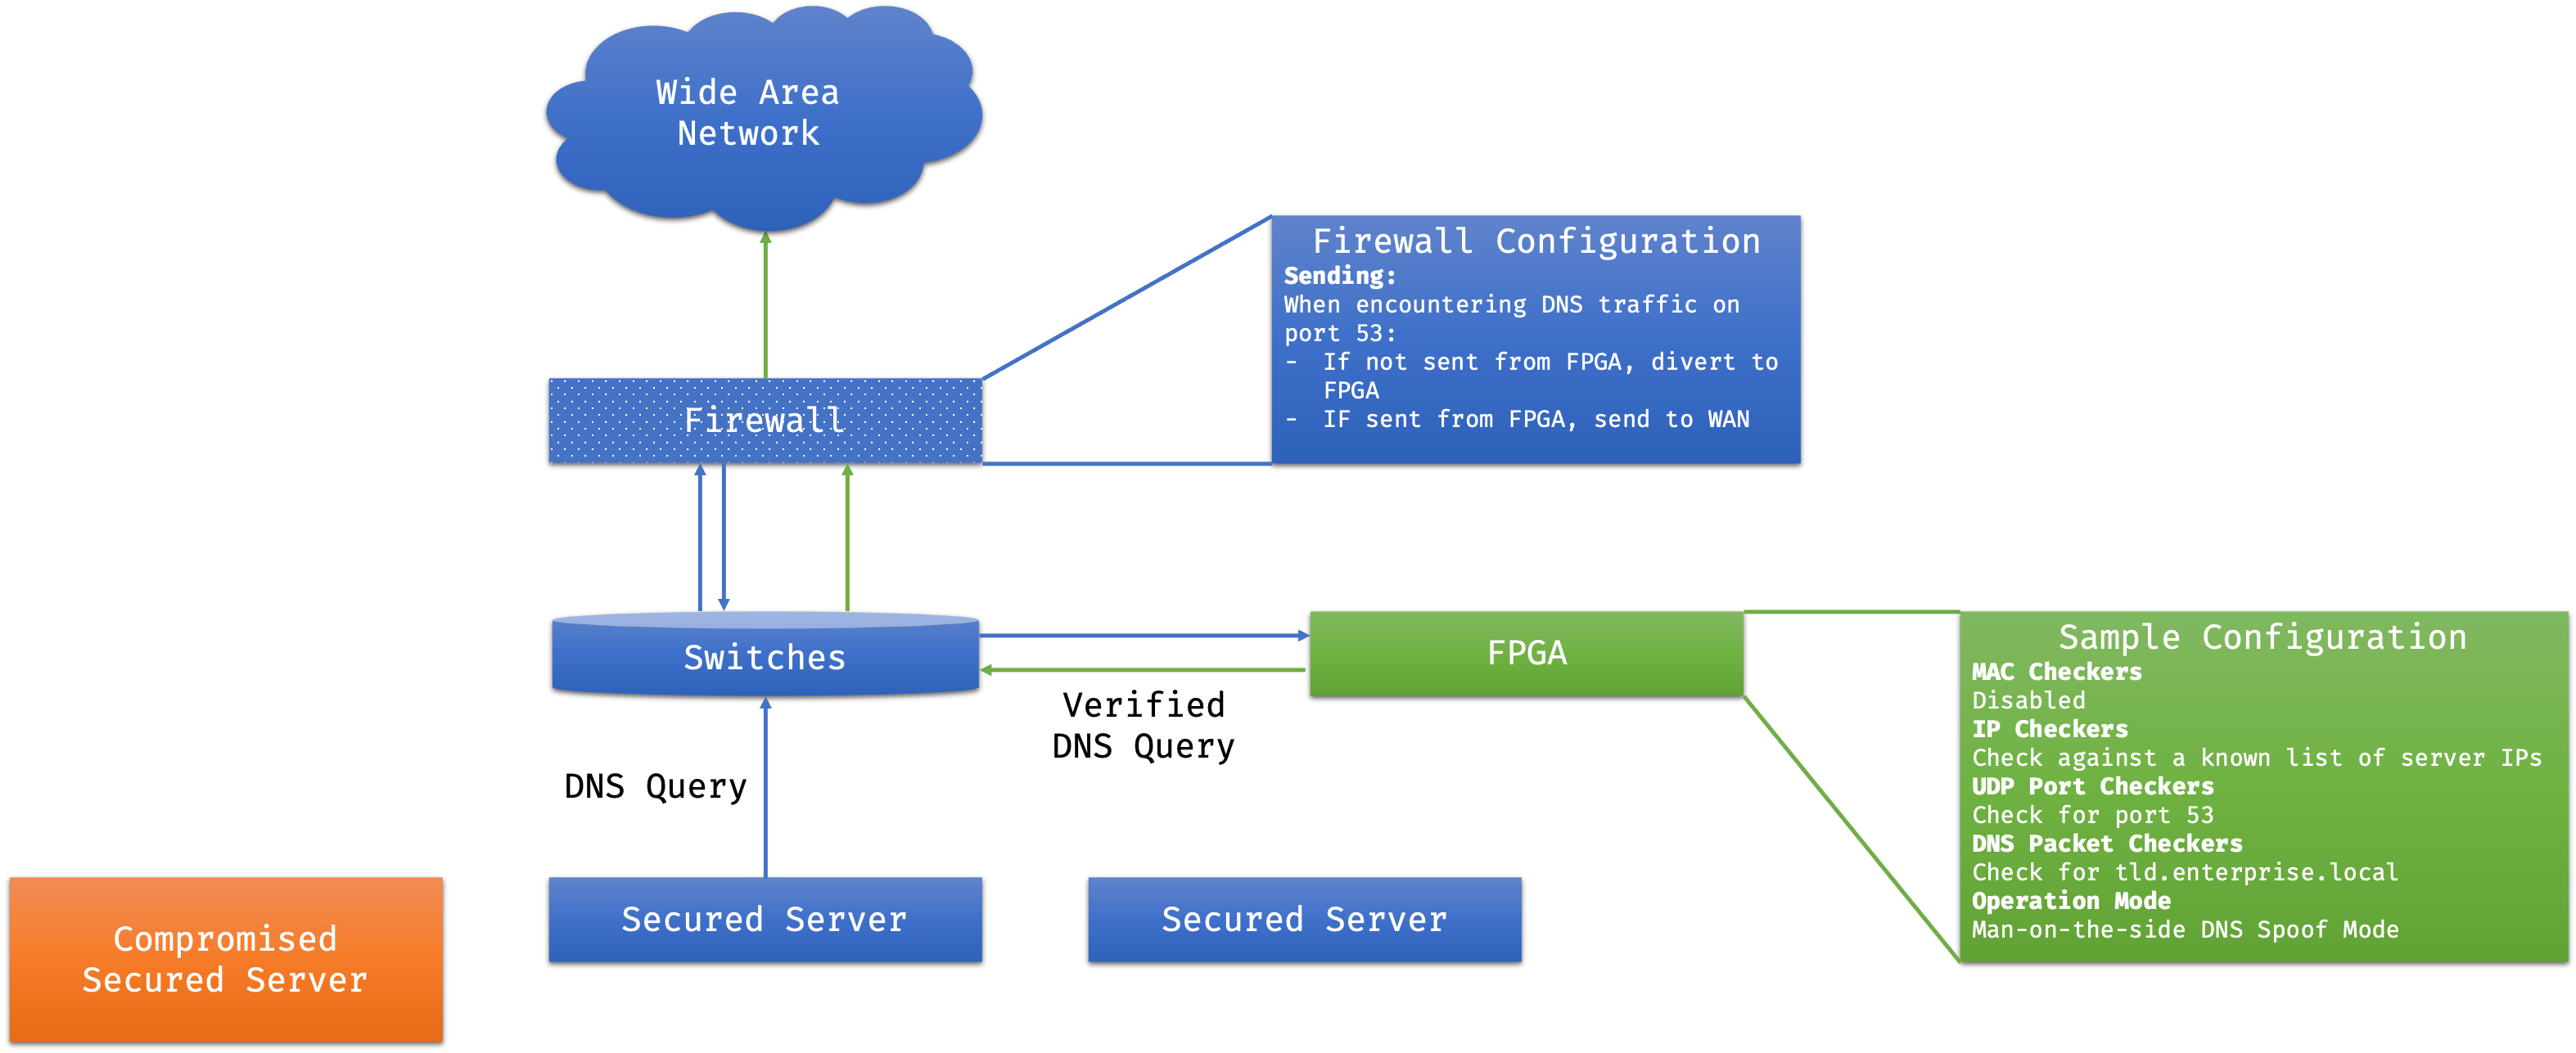
\includegraphics[width=1.1\textwidth]{imgs/man-on-the-side-valid-dns-query.png}}
  \caption{Man-on-the-Side FPGA sample topology - Sending legitimate DNS query}
  \label{fig:man-on-the-side-FPGA-send-legit}
\end{figure}

Legitimate DNS queries would not be affected within the network, as shown in Figure \ref{fig:man-on-the-side-FPGA-send-legit}. The packet will first be redirected to the FPGA for security checks. Once the FPGA deems the packet legitimate, it will forward the packet to the firewall, dispatching the packet to the upstream network. 

\begin{figure}[H]
  \makebox[\textwidth][c]{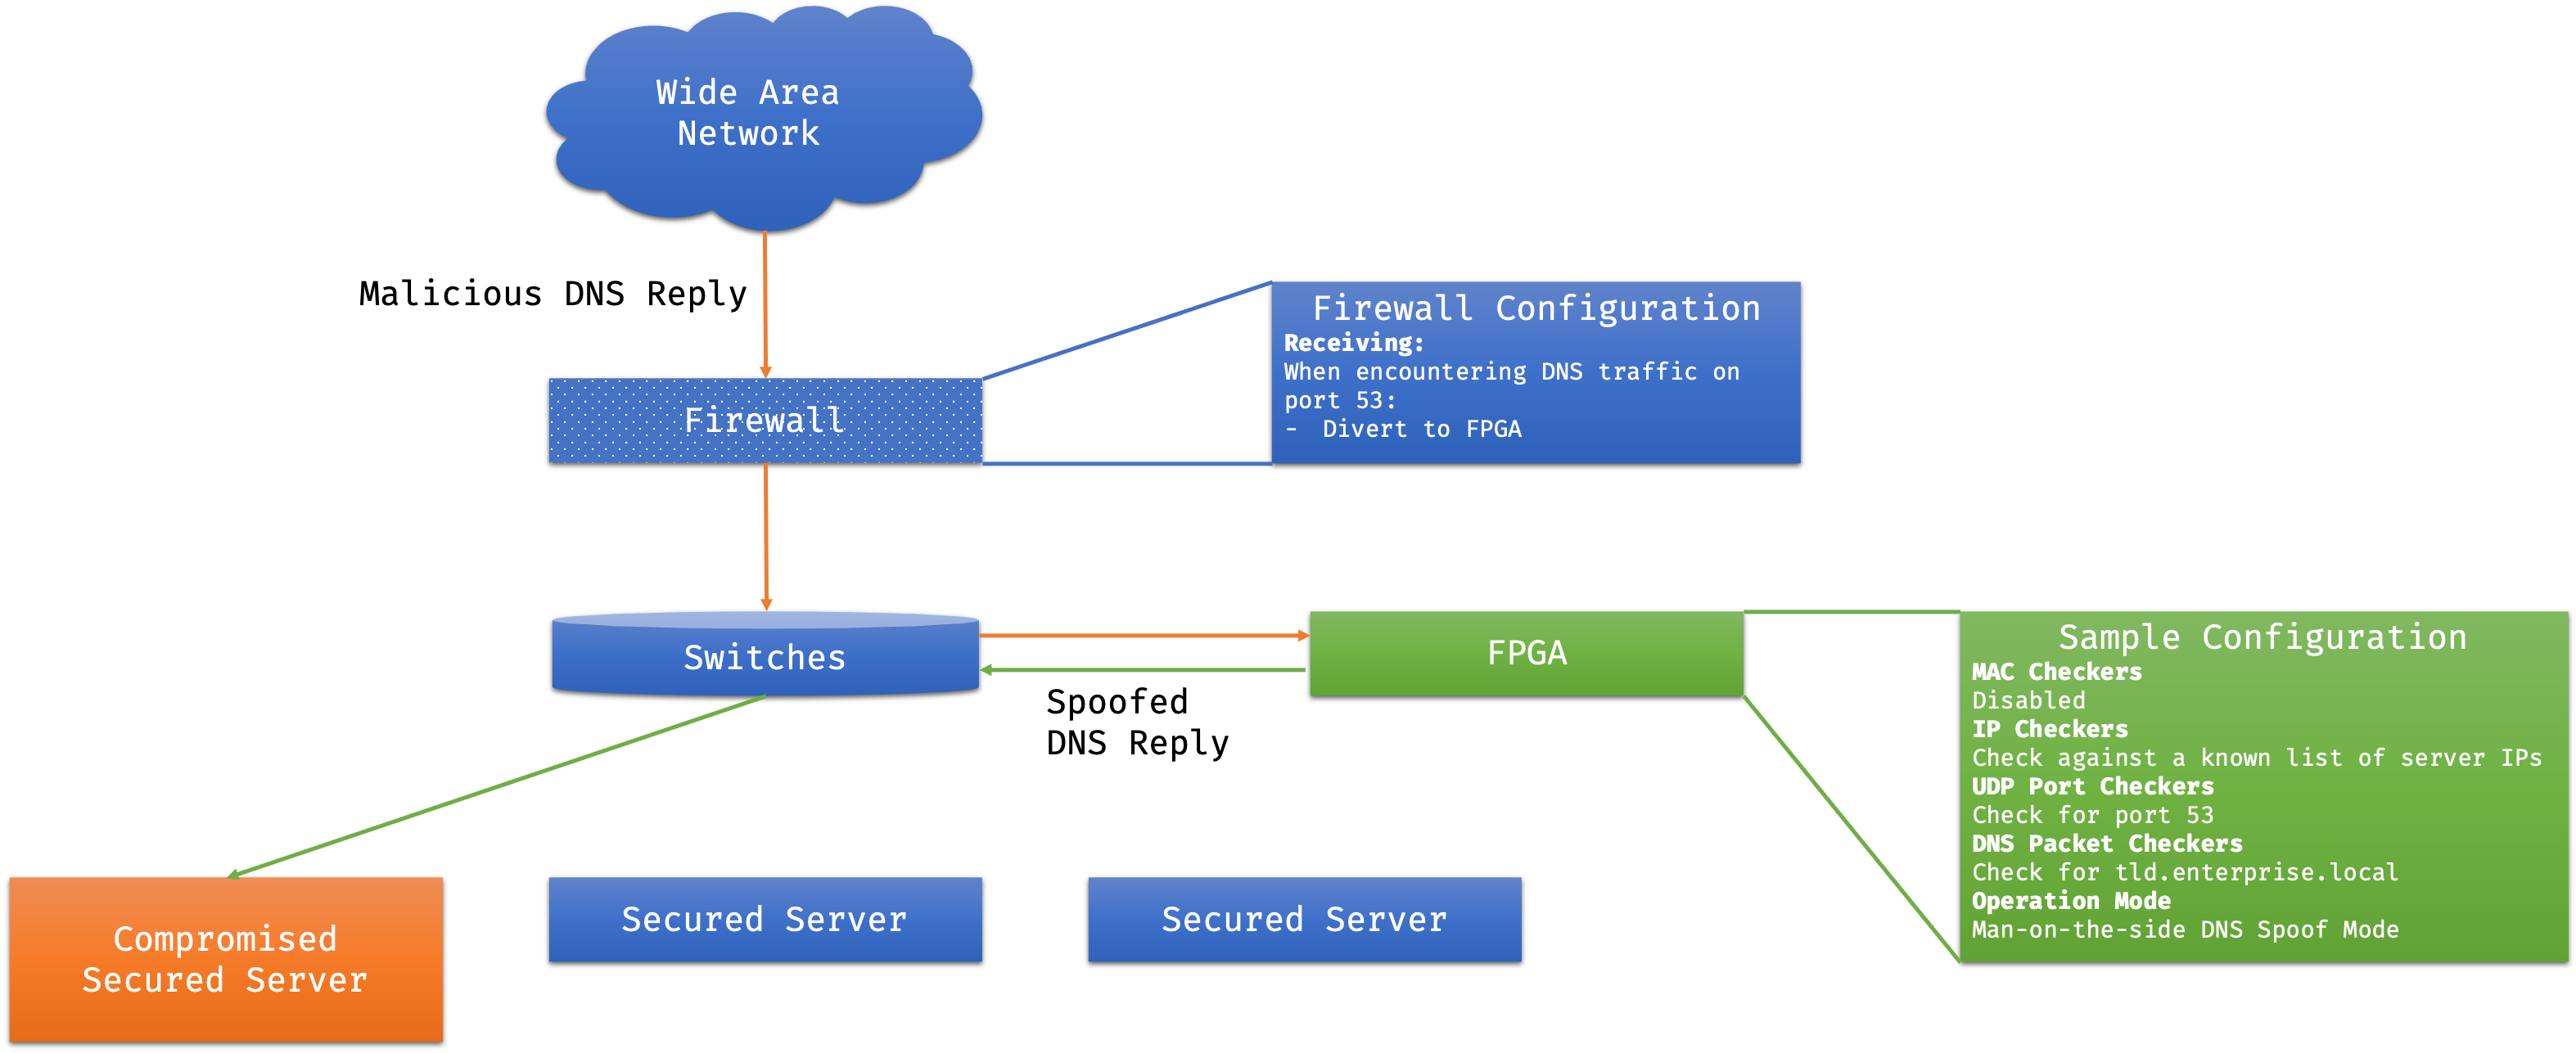
\includegraphics[width=1.1\textwidth]{imgs/man-on-the-side-malicious-dns-reply.png}}
  \caption{Man-on-the-Side FPGA sample topology - Receiving malicious DNS exfiltration / tunnelling reply}
  \label{fig:man-on-the-side-FPGA-recv-malicious}
\end{figure}

In the sporadic case where a malicious DNS exfiltration/tunnelling query did get sent to the attacker's C\&C due to unknown issues, the reply can still be blocked by the FPGA if configured correctly. In the case where the networks receive a DNS remote control reply, the firewall would divert the packet to FPGA for examination. The checker in the FPGA would fail, and this would also trigger a spoofed DNS reply sent to the compromised host, as shown in Figure \ref{fig:man-on-the-side-FPGA-recv-malicious}.

\begin{figure}[H]
  \makebox[\textwidth][c]{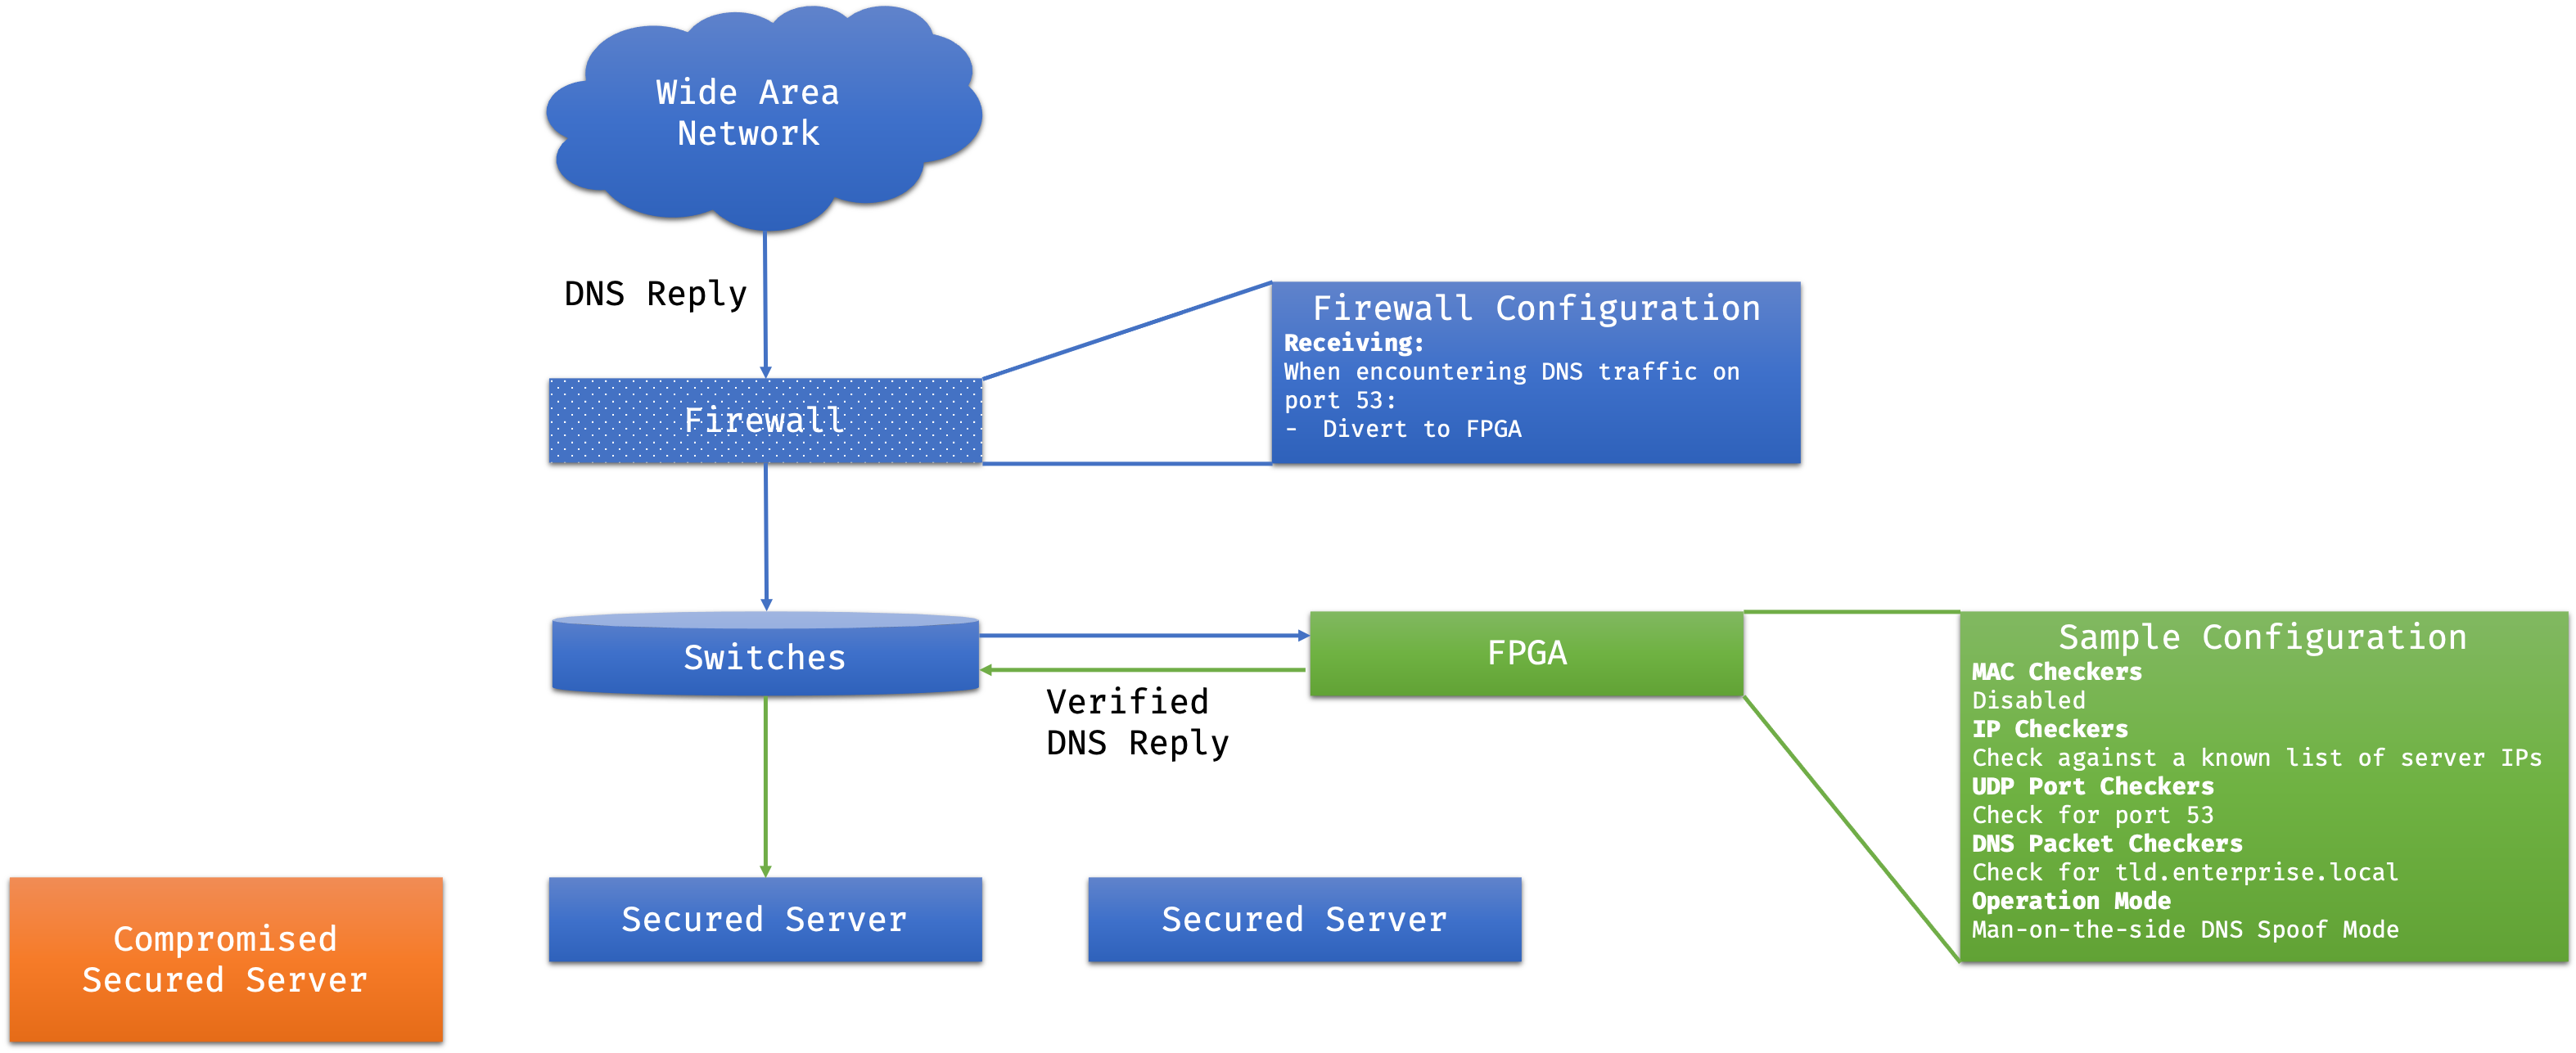
\includegraphics[width=1.1\textwidth]{imgs/man-on-the-side-valid-dns-reply.png}}
  \caption{Man-on-the-Side FPGA sample topology - Receiving legitimate DNS reply}
\end{figure}

As expected, legitimate DNS responses would remain unaffected throughout the process except for a minimal overhead added by the FPGA scrutinising the packet. The reply will be received by the firewall, forwarded to the FPGA. The FPGA will inspect the packet rapidly and deliver the verified response to the intended host untouched.

\subsection{DNS Flood}

This FPGA-based system can also be used to counter DNS flood attack on DNS name servers. As specified in Figure \ref{fig:dns-flood-man-in-the-middle}, we deploy the system in a man-in-the-middle manner in front of the DNS name servers. The FPGA operation mode is set to ``Man-in-the-middle Filter", which would forward the same payload upon passing the filter. With regards to the filters, we can configure them as:

\begin{itemize}
    \item MAC filters: Allow trusted Ethernet MACs from upstream ISP providers
    \item IP filters: Block a list of known IP address sending malicious IP addresses
    \item UDP Port filters: Allow only DNS port 53
    \item DNS filters: Allow only whitelisted domain names and block all unknown domain names
\end{itemize}

Notably, we are placing the FPGA system as a hardware-based simple Layer 7 filter in front of the system's software-based firewall. Utilising the unparalleled packet processing speed of FPGAs, most flood traffic can be examined, logged and discarded by the FPGA with minimal latency before reaching the software firewall. Moreover, FPGAs can be scaled up linearly without extra overhead to accept and filter more flood traffic by simply connecting more FPGAs in parallel between the WAN and the software firewall. Therefore, the software firewall would enjoy a much lower network load when under attack, as a large percentage of the junk traffic would already have been blocked by the FPGAs. Thus, more complex checks can be performed by the software firewall with its spare CPU time. With this setup, we can make sure the DNS name servers are well-protected with minimal performance and latency impact on the overall system.

\begin{figure}[H]
  \makebox[\textwidth][c]{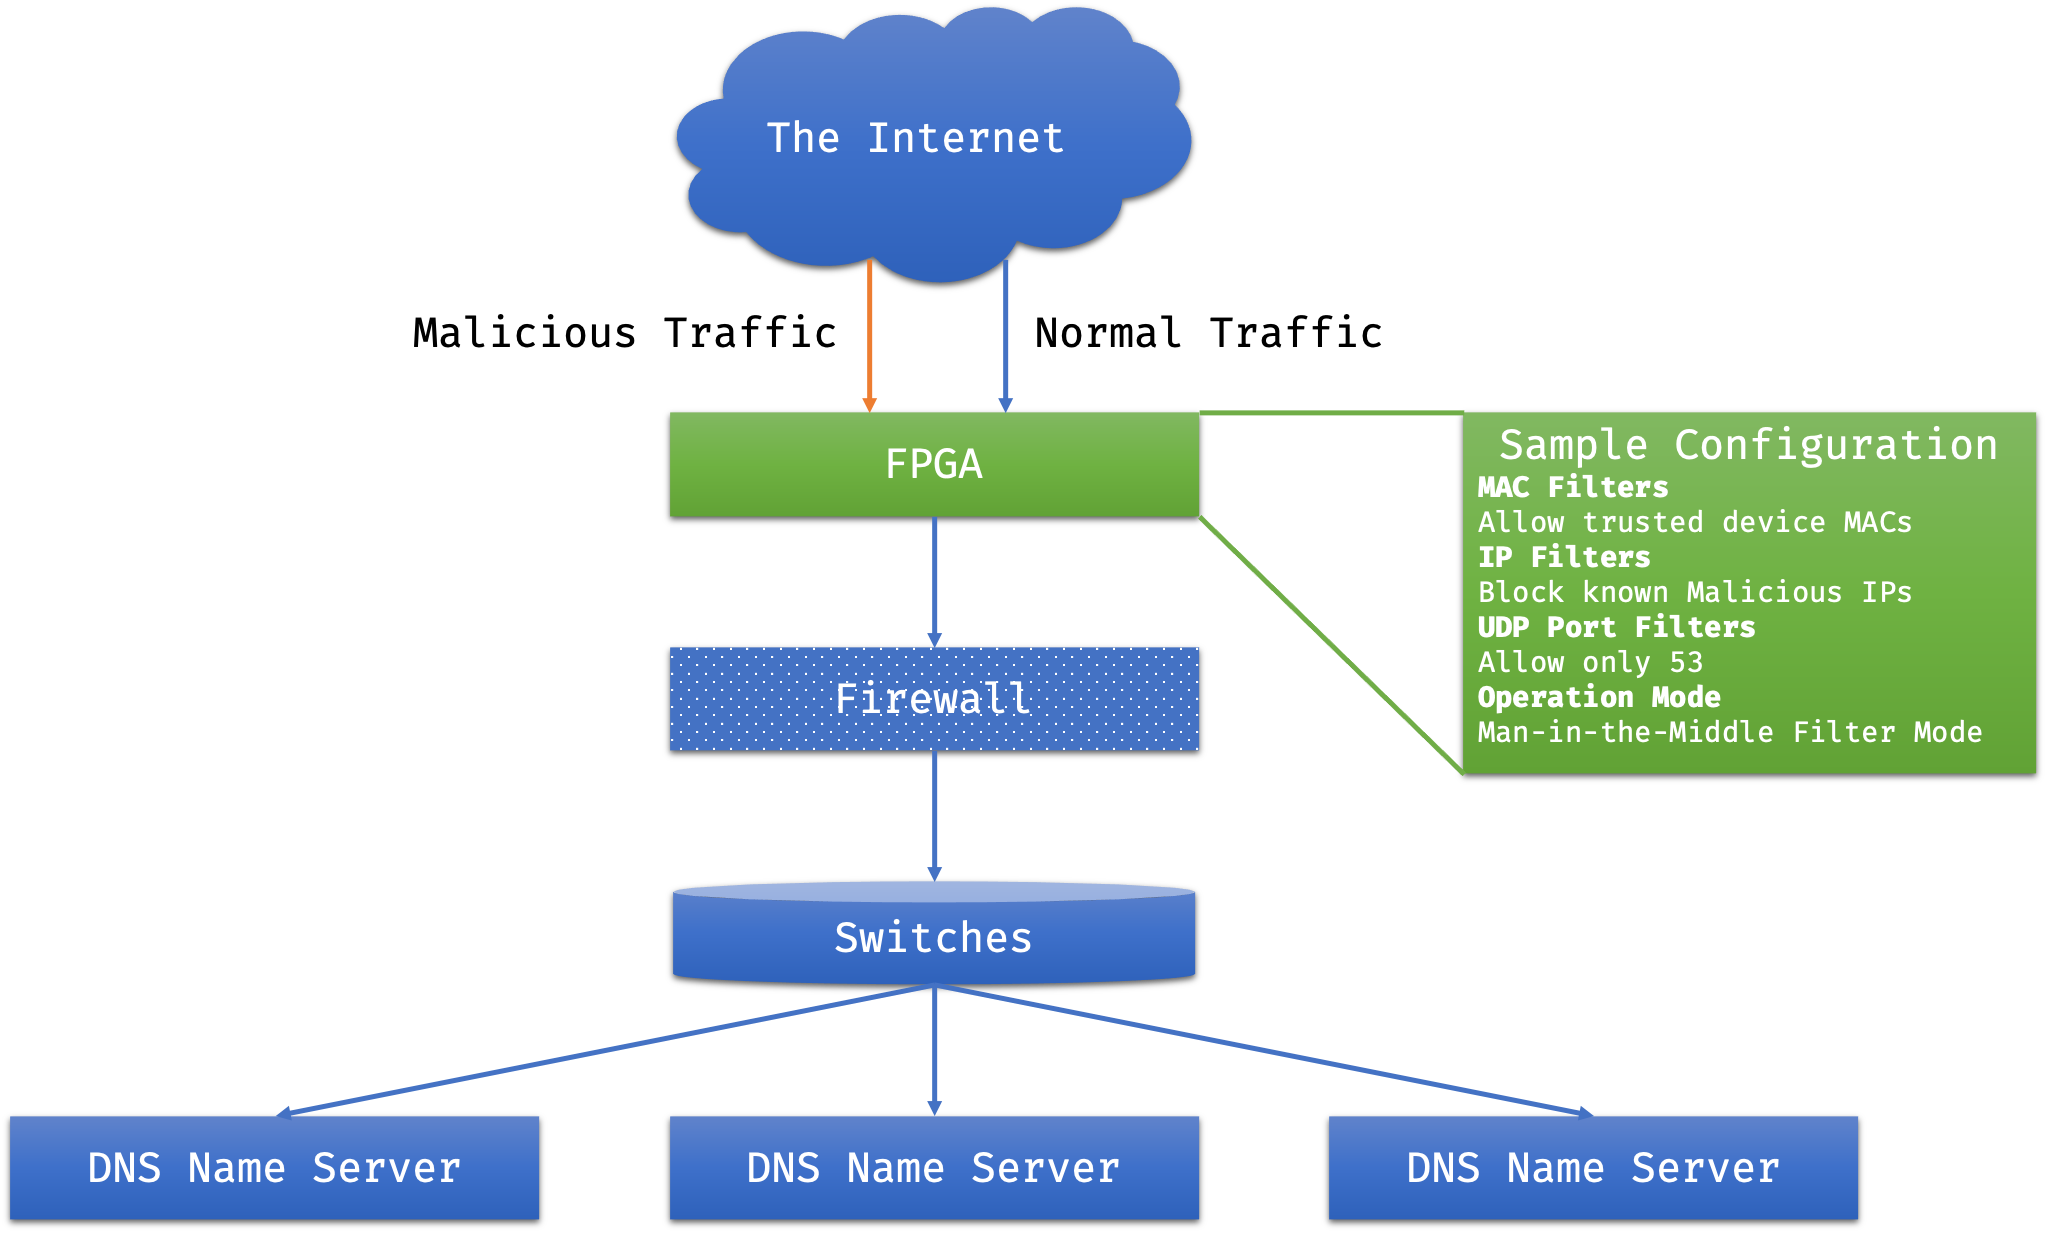
\includegraphics[width=0.8\textwidth]{imgs/man-in-the-middle-topology.png}}
  \caption{Man-in-the-Middle DNS Name Server FPGA sample topology - FPGA in the middle}
  \label{fig:dns-flood-man-in-the-middle}
\end{figure}

When it comes to multi-purposed networks that serve not only DNS queries, the aforementioned topology in Figure \ref{fig:dns-flood-man-in-the-middle} might not be the best solution since all traffic except DNS is discarded by the FPGA. Instead, we can resort to the sample topology shown in Figure \ref{fig:dns-flood-man-in-the-middle-asic}. In this approach, we put FPGA on the side of the network, only monitoring DNS transactions. Technically, this approach should be no different as FPGA is still in the middle of all DNS traffic. The incoming traffic from WAN would ideally pass through an ASIC-based Layer 3 firewall that diverts all DNS traffic to the FPGA and keeps other traffic on the usual route towards a Layer 7 firewall or directly towards a switch (in a less secure environment). Like the previous configuration, the FPGA would detect, log and drop packets not meeting the filter requirements. Legitimate payloads are expected to pass the filter and be forwarded directly to the switch.

\begin{figure}[H]
  \makebox[\textwidth][c]{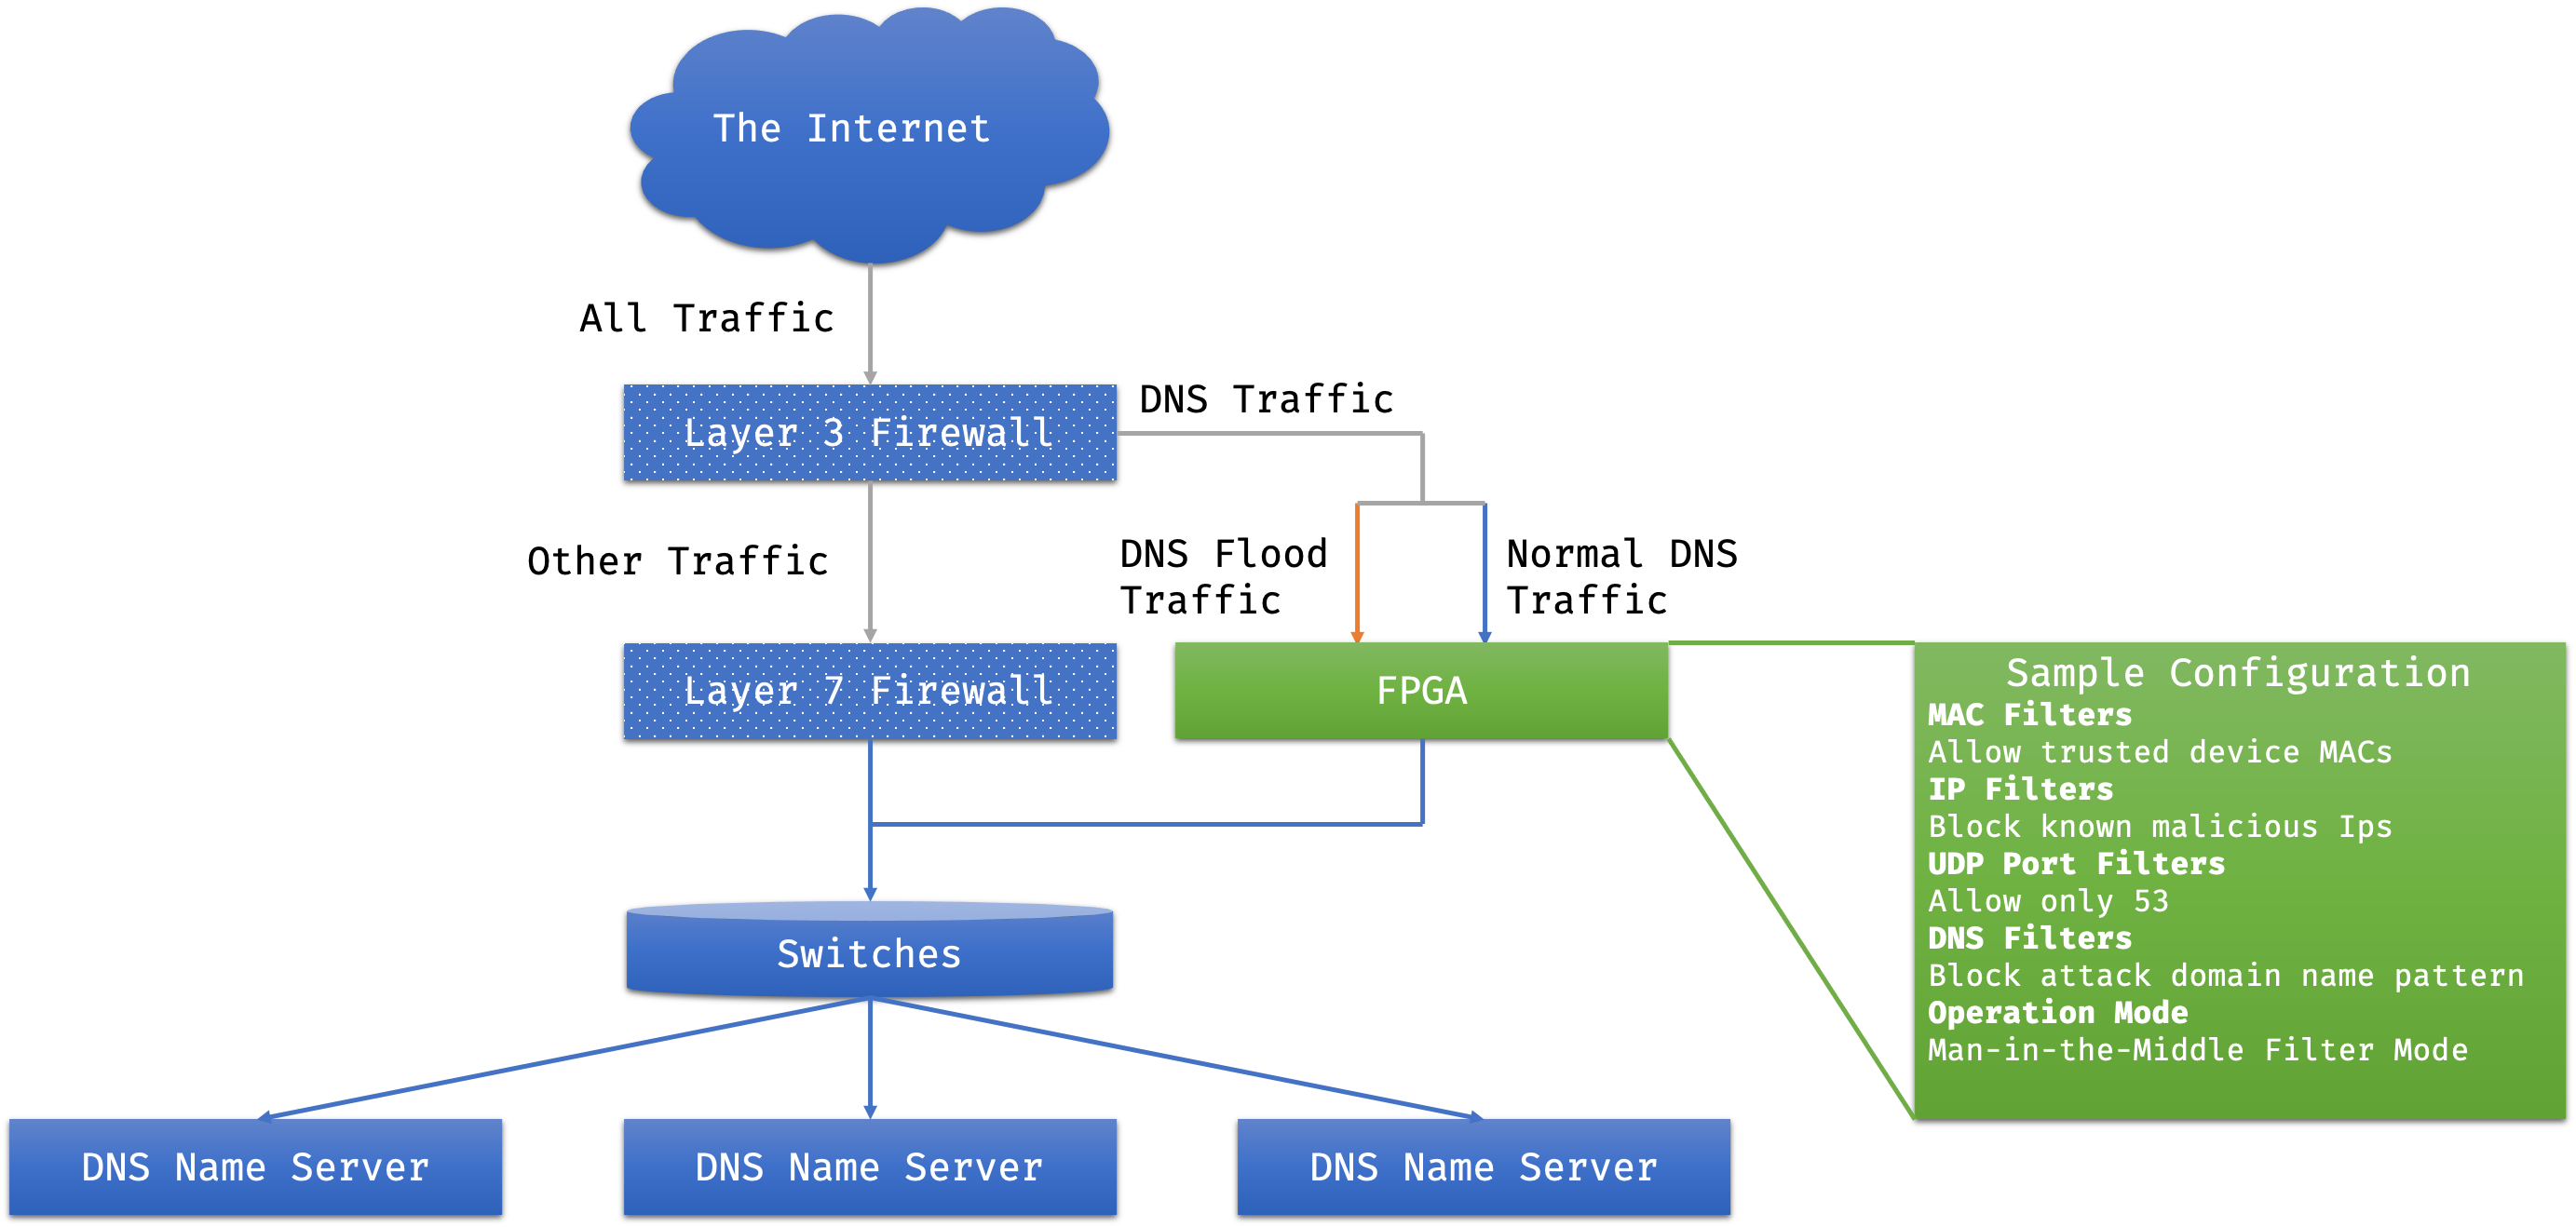
\includegraphics[width=1.1\textwidth]{imgs/man-in-the-middle-amp-topology.png}}
  \caption{Man-in-the-Middle DNS Name Server FPGA sample topology - FPGA on the side}
  \label{fig:dns-flood-man-in-the-middle-asic}
\end{figure}

\section{Design Summary}

As shown in the discussions above, we designed our hardware and software with performance as the top priority, without any substantial loss of scalability and flexibility. The topology samples demonstrate the FPGA-based system's capability to adapt to networks of all sizes and provide an extra level of DNS security and defence in real-time with minimal latency overhead.

\chapter{Implementation}

In this chapter, we will be discussing implementation details of the FPGA-based system, including hardware engineering and debugging processes, as well as software development and integration steps.

\section{Hardware Implementation}
\label{section:implementation-hardware-implementation}

\begin{figure}[H]
  \makebox[\textwidth][c]{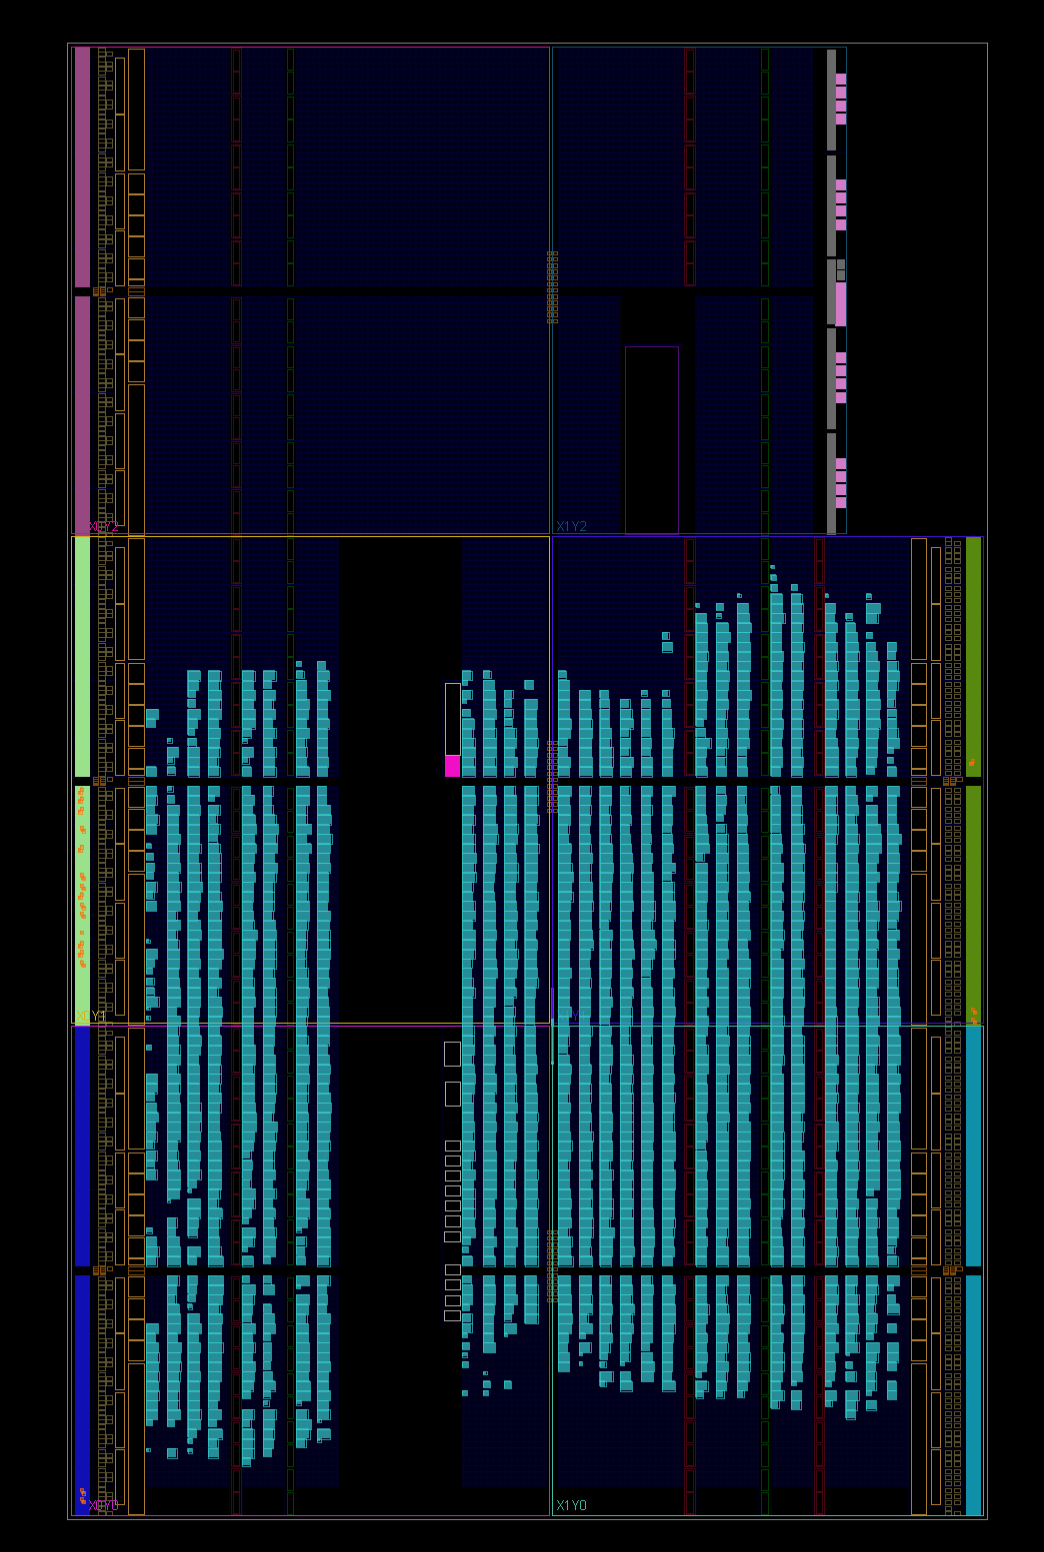
\includegraphics[angle = 90, width=0.72\textwidth]{imgs/on-chip-impl.png}}
  \caption{Final Chip Implementation of the system on Artix-A7 (XC7A35TICSG324-1L)}
  \label{fig:on-chip-impl}
\end{figure}

\subsection{Finite State Machine (FSM) Implementation}

\begin{figure}[h!]
  \makebox[\textwidth][c]{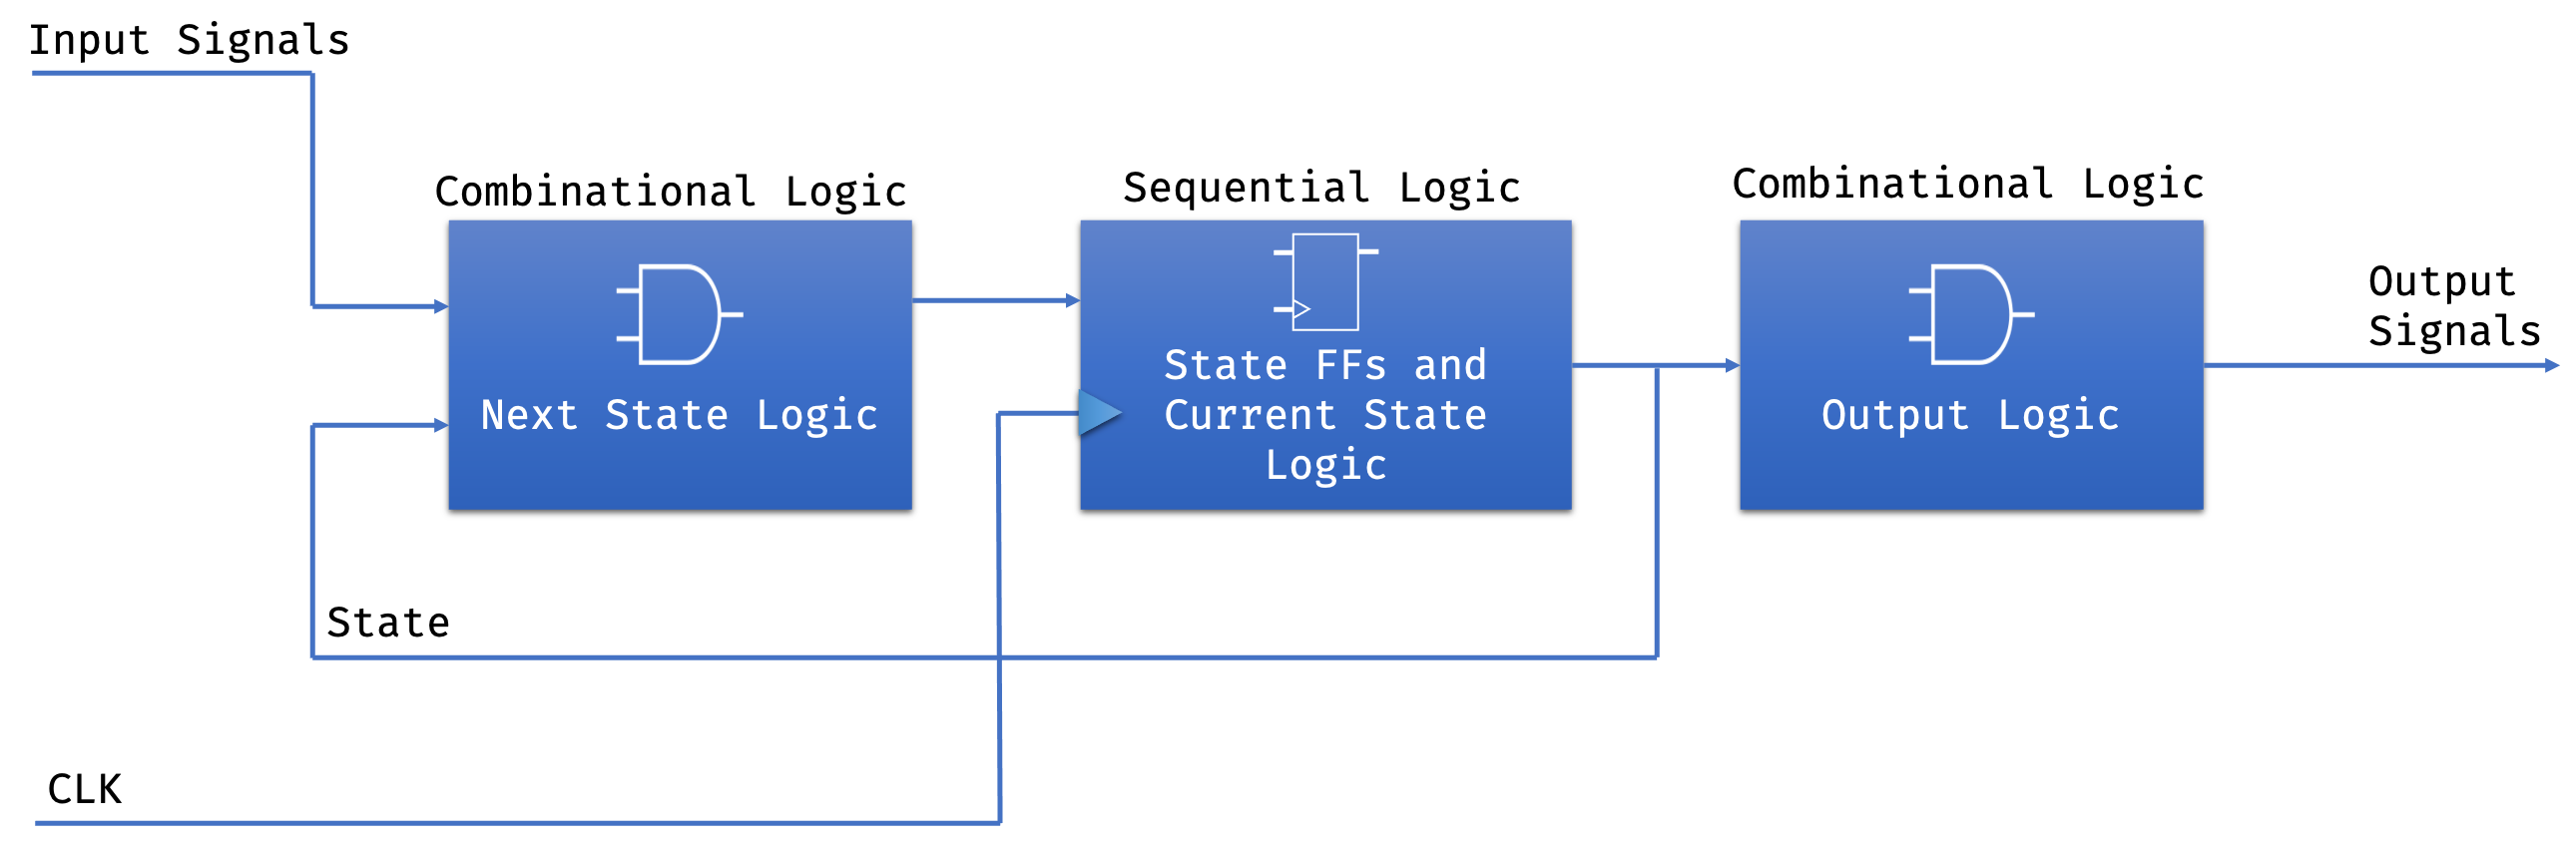
\includegraphics[width=\textwidth]{imgs/FSM-impl.png}}
  \caption{Final State Machine Hardware Implementation}
  \label{fig:fsm-impl}
\end{figure}

FSM is one of the most commonly used design technique in stateful logic hardware circuits. More specifically, a hardware implementation of a $n$-state FSM requires three main logic blocks, as shown in Figure \ref{fig:fsm-impl}:
\begin{itemize}
    \item Next State Logic: a block of combinational circuit to determine the next state.
    \item State FFs and Current State Logic: a set of registers storing state information and a sequential logic circuit operating input signals based on the state. The number of FFs used is dependent on the encoding method, varying from $\ceil*{\log_2 n}$(binary encoded) - $n$(one-hot encoded).
    \item Output Logic: another stateless combinational circuit to output processed signals.
\end{itemize}

\begin{figure}[h!]
    \centering
    \begin{minipage}{0.32\textwidth}
        \centering
        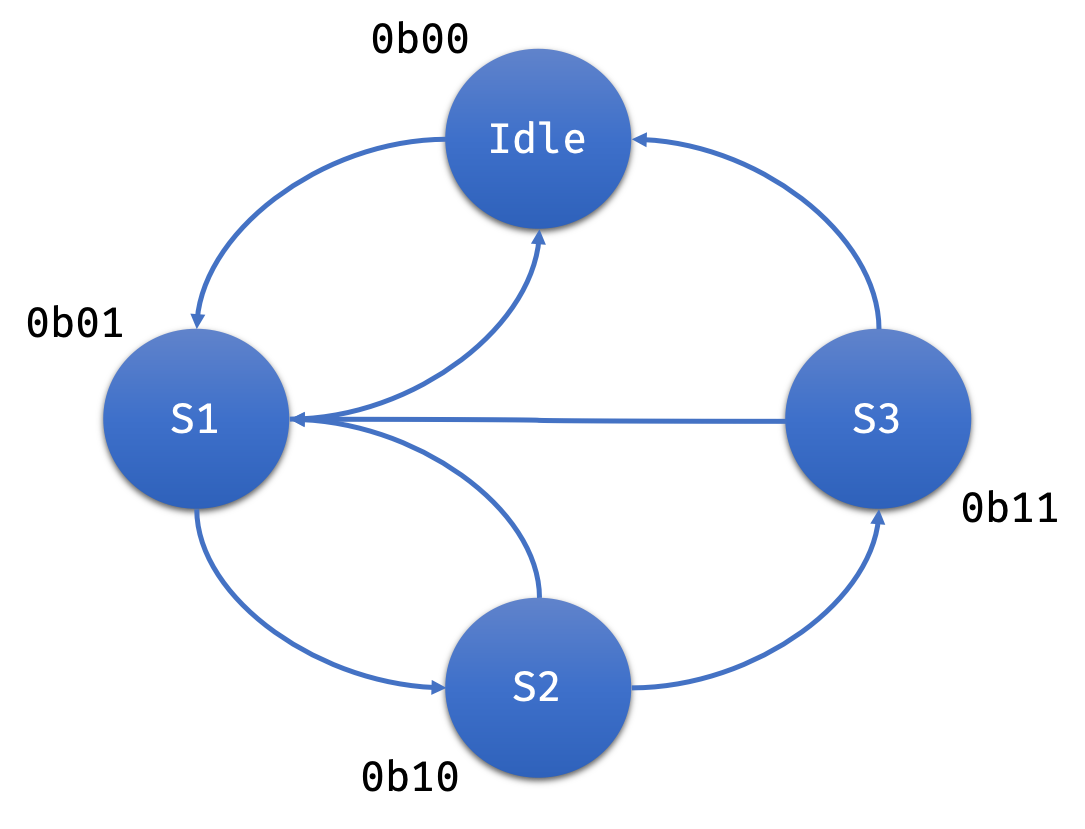
\includegraphics[width=\linewidth]{imgs/binary-encoding-fsm.png}
    \end{minipage}%
    \begin{minipage}{0.32\textwidth}
        \centering
        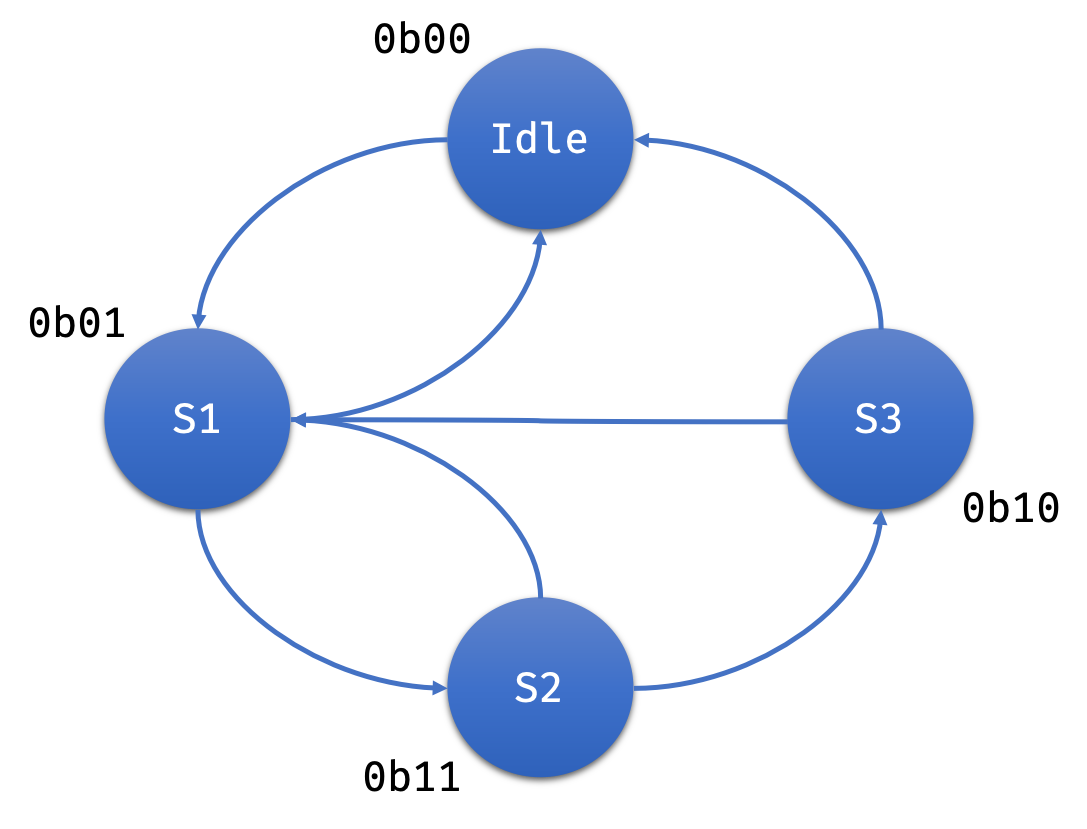
\includegraphics[width=\linewidth]{imgs/grey-encoding-fsm.png}
    \end{minipage}
    \begin{minipage}{0.35\textwidth}
        \centering
        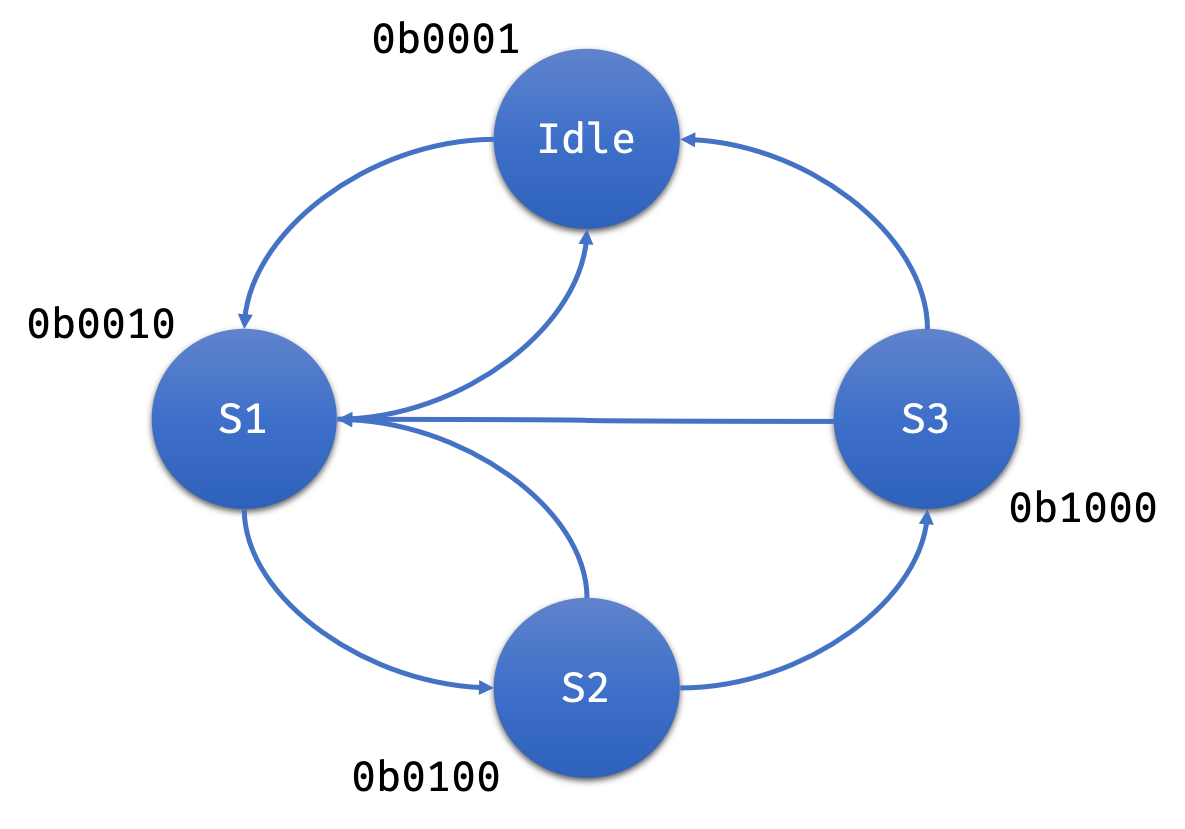
\includegraphics[width=\linewidth]{imgs/one-hot-fsm.png}
    \end{minipage}
    \caption{Binary-Encoded, Grey-Encoded and One-Hot-Encoded FSM}
    \label{fig:binary-grey-one-hot-encoded-FSM}
\end{figure}

Regarding the number of FFs in the state register, there are three main encoding methods shown in Figure \ref{fig:binary-grey-one-hot-encoded-FSM}, namely binary encoding, grey encoding and one-hot encoding.

Binary encoding is the most intuitive when assigning a numerical value to sequential states, and we are using as few bits as possible to encode the states. For an $n$-state FSM, binary encoding them sequentially yields $\ceil*{\log_2 n}$ bits. With the $4$-state FSM shown on the left side of Figure \ref{fig:binary-grey-one-hot-encoded-FSM}, $\ceil*{\log_2 4} = 2$ FFs would be needed. Binary encoding uses the least amount of memory, but the transitions can be very strict with timing\footnote{See Section \ref{section:implementation-hardware-debugging} for more information on hardware timing constraints \label{foot:timing-constraints}} in cases like going from $\mathtt{0x7f}$ to $\mathtt{0x80}$, with 8 bits to drive within one clock cycle (7 bits to set 0 and 1 bits to set 1).

Grey encoding consists of a sequence where only one bit changes between the current value and next. This encoding developed aiming to minimise the bit flips when transitioning between states so as to further relieve the timing constraints and reduce dynamic power consumption\footref{foot:timing-constraints}. Notice the difference of encoding at State $S2$ and $S3$ in between the left FSM and the middle FSM in Figure \ref{fig:binary-grey-one-hot-encoded-FSM}, the grey-encoded FSM encodes $S2$ as $\mathtt{0b11}$ instead of $\mathtt{0b10}$ to ensure $S1 (\mathtt{0b01})\xrightarrow{}S2(\mathtt{0b11})$ flips only one bit, and similarly for $S2 (\mathtt{0b11})\xrightarrow{}S3(\mathtt{0b10})$.

Lastly, one-hot encoding is a scheme in which each bit represents one single state. Thus, at any point in time, there can only be one VCC (1) in states, while all other bits are Ground (GND) (0). With reference to the $4$-state FSM on the right side of Figure \ref{fig:binary-grey-one-hot-encoded-FSM}, the four states are encoded as $\mathtt{0b0001}$, $\mathtt{0b0010}$,  $\mathtt{0b0100}$ and $\mathtt{0b1000}$. This encoding method seems inefficient as encoding a $n$-state FSM requires $n$ FFs. However, one-hot encoding is particularly useful in strict timing scenarios and simplifies the stimulus logic\footref{foot:timing-constraints}. The bits represent the states directly, and there is no state-decoding delay.

\begin{lstlisting}[language=VHDL, caption=One-Hot Encoded FSM Minimal Example in \proglang{VHDL}, label={lst:one-hot-fsm-minimal}]
TYPE state_t IS (IDLE, START, RUN, DONE);

ATTRIBUTE enum_encoding : STRING;
ATTRIBUTE enum_encoding OF state_t : TYPE IS "one-hot";

SIGNAL s, sin : state_t;

stim : PROCESS (clk)
BEGIN
  IF rising_edge(clk) THEN
    CASE s IS
      WHEN IDLE =>
        sin <= START;
      WHEN START =>
        sin <= RUN;
      WHEN RUN =>
        sin <= DONE;
      WHEN DONE =>
        sin <= IDLE;
    END CASE;
  END IF;
END PROCESS;

reg : PROCESS (clk)
BEGIN
  IF falling_edge(clk) THEN
    s <= sin;
  END IF;
END PROCESS;
\end{lstlisting}

Typically, we can provide a behavioural description of the FSM states in \proglang{VHDL} and the synthesiser would be able to decide the encoding based on the complexity of the algorithm and the number of states. However, in some instances where timing constraints are strict, we will have to specify encoding methods precisely by providing a signal description of the state registers.

Listing \ref{lst:one-hot-fsm-minimal} is a minimal example of One-Hot Encoded FSM in \proglang{VHDL}. Note that, at line $4$, we set the attribute specifically to \code{one-hot}, and the synthesiser would generate a One-Hot-Encoded FSM netlist accordingly. It is also worth noting that we store state \code{s} changes in signal \code{sin} on a rising clock edge and refresh the current state \code{s} on a falling edge. This is an attempt to make sure signal \code{s} would not run into metastability in a clock cycle when it is instantly used after modification\footnote{See Section 4.2 for more information on signal metastability in hardware}.

FSM is implemented in most components within the FPGA-based system. Parsing, processing and constructing network packets are all sequential logic and fit nicely with the stateful design of FSM.

\subsection{Top Level Module and Clock Divider}
\label{section:implementation-hardware-implementation-top-level-clock-divdier}

Figure \ref{fig:top-level-design} shows the implemented top-level design of the FPGA. As a streamlined packet processing system, the components are connected linearly as the packet flows from the incoming PHY receiver to the outgoing PHY transmitter.

\begin{landscape}
\begin{figure}[h!]
  \centering
  \includegraphics*[viewport={0 0 950 600}, height=\textwidth, width=2\textheight, keepaspectratio]{imgs/top-level-module.png}
  \caption{Top Level Module Overview - 1}
  \label{fig:top-level-design}
\end{figure}
\begin{figure}[h!]
  \ContinuedFloat
  \centering
  \includegraphics*[viewport={950 0 1900 600}, height=\textwidth, width=2\textheight, keepaspectratio]{imgs/top-level-module.png}
  \caption{Top Level Module Overview - 2}
  \label{fig:top-level-design}
\end{figure}
\begin{figure}[h!]
  \ContinuedFloat
  \centering
  \includegraphics*[viewport={1900 0 2850 600}, height=\textwidth, width=2\textheight, keepaspectratio]{imgs/top-level-module.png}
  \caption{Top Level Module Overview - 3}
  \label{fig:top-level-design}
\end{figure}
\end{landscape}

\begin{lstlisting}[language=VHDL, caption=Snippet of Clock Divider \code{clock.vhd}, label={lst:clock-vhd}]
ARCHITECTURE rtl OF clock IS
  SIGNAL clk_divider : unsigned(1 DOWNTO 0) := (OTHERS => '0');
BEGIN

  div : PROCESS (i_clk)
  BEGIN
    IF (rising_edge(i_clk)) THEN
      clk_divider <= clk_divider + 1;
    END IF;
  END PROCESS div;

  o25_clk <= clk_divider(1);
  o50_clk <= clk_divider(0);
 
END rtl;
\end{lstlisting}

As seen at the bottom of left of Figure \ref{fig:top-level-design}, \code{inst\_clock} is the clock divider component of the system. With reference to the Digilent Arty A7-35T manual\cite{digilent-arty}, a single crystal oscillator of $100$ MHz is connected to the board via pin E3. Considering system stability and overall design difficulties, we set the Artix-7 FPGA core to the default $50$ MHz Speedgrade 1 as per Xilinx clocking documentation \cite{xilinx-7-clocking}. Moreover, the interfacing PHY chip, Texas Instruments (TI) DP83848J, operates under a $25$ MHz clock when using MII ($50$ MHz when using Reduce MII (RMII)), which needs to be generated by the circuit and sent to pin X1\cite{texas-instruments-dp83848x}. Therefore, we would need to introduce an oscillator signal processor to generate the clock we want in different system domains. As laid out in Listing \ref{lst:clock-vhd}, The clock divider operates upon the rising edge of the oscillator and produces a slower clock using an internal unsigned rollover counter. Note that the clock divider is implemented as simply as possible without overflow checks to minimise the processing skew added to the FPGA fast clock path.

\subsection{PHY MII-family Interface, Receiver and Sender Peripheral}
\label{section:implementation-hardware-implementation-phy-mac-peripheral}

As described earlier, Arty-A7 35T has an on-chip Ethernet PHY ASIC peripheral (TI DP83848J), which operates under two interfaces, two Cat-5 speed grades and two duplex modes: RMII / MII, $10$ / $100$ Mbps and half/full duplex, respectively \cite{texas-instruments-dp83848x}. All three settings can be configured via functional pins \code{LED\_LINK}, \code{LED\_SPEED} and \code{MII\_MODE}. In this project, we configure the PHY chip to operate with an MII interface, $100$ Mbps full-duplex PHY link.

The MII-family interface is standard by IEEE 802.3u \cite{ieee802.3ethernet-2018} as the interface to connect an Ethernet Media Access Control (MAC) block to a PHY ASIC. It is considered a universal abstraction interface above various physical network media (i.e. twisted pair, fibre optic, etc.). With the MII-family interface, any MAC hardware/software can connect to any PHY independent of the network signal transmission media.

The main receiving and transmitting signals on the interface includes:
\begin{itemize}
    \item \code{CRS}: Carrier Sense
    \item \code{COL}: Collision, which would not be used in full-duplex connections
    \item \code{RX\_CLK}, \code{TX\_CLK}: Receive / Transmit Clock
    \item \code{RXD[0-3]}: Receive Data [0-3],  (4 bits per clock cycle)
    \item \code{TXD[0-3]}: Transmit Data [0-3],  (4 bits per clock cycle)
    \item \code{RX\_DV}: Receive Data Valid (GND on this signal means data received on \code{RXD[0-3]} are just noise on the PHY)
    \item \code{TX\_EN}: Transmit enable (VCC on this signal means data provided on \code{TXD[0-3]} will be sent to the wire)
    \item \code{RX\_ER}, \code{TX\_ER}: Receive / Transmit Error (VCC on this signal means the PHY has received undecodable data / was unable to transmit data, possibly due to broken connections or unsuccessful negotiations)
\end{itemize}

\begin{figure}[h!]
  \makebox[\textwidth][c]{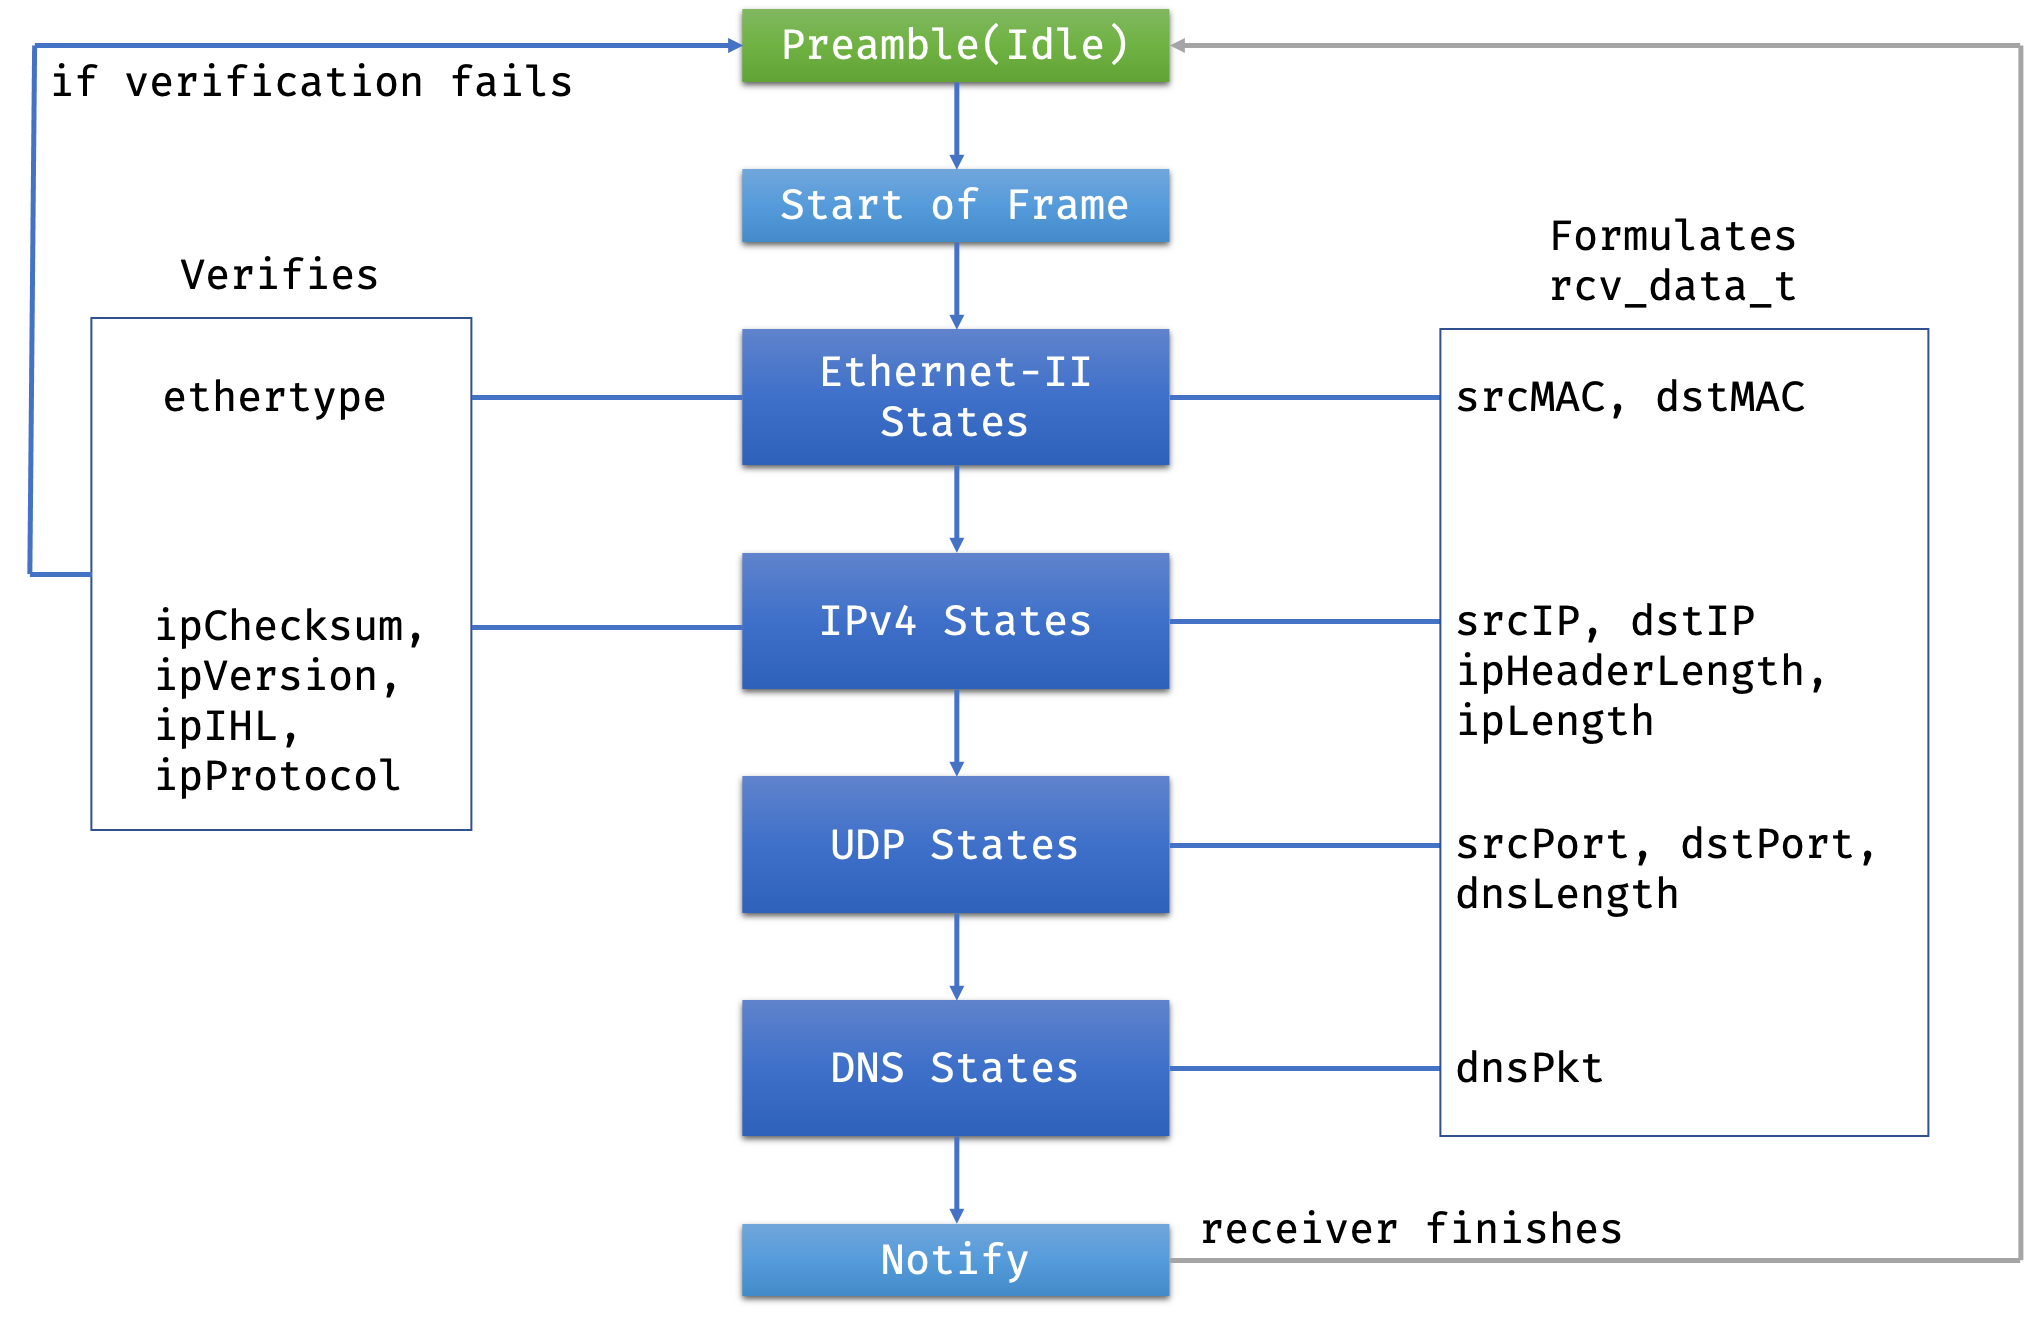
\includegraphics[width=0.8\textwidth]{imgs/rcv-fsm.png}}
  \caption{\code{mac\_rcv.vhd} Module FSM Overview}
  \label{fig:rcv-fsm}
\end{figure}

Using the FSM sequential logic, we implemented our Receiver FSM as shown in Figure \ref{fig:rcv-fsm}. When \code{RX\_DV} is at VCC level, the receiver starts listening for Ethernet-II preambles at state \code{Preamble} and proceeds with state transitions accordingly. During the parsing states, the receiver analyses the packet as nibbles (4 bits) coming in from \code{RXD}, forms a \code{rcv\_data\_t} and checks for packet correctness at numerous checkpoints, including \code{ethertype}, \code{ipChecksum} and etc. As mentioned previously in design Section \ref{section:design-system-design-hardware}, the \code{dnsPkt} struct is limited to $1024$ bits (128 bytes) for the ease of signal transfer across components under strict timing requirements at the \code{Notify} state. Therefore, all bytes above this limit will be cut off and discarded beyond the receiver. Once all input verification passes and the struct \code{rcv\_data\_t} is properly constructed, the component would notify its predecessor by setting \code{EL\_DV} to high and return to the state \code{Preamble(Idle)}, ready for the next packet.

\begin{figure}[h!]
  \makebox[\textwidth][c]{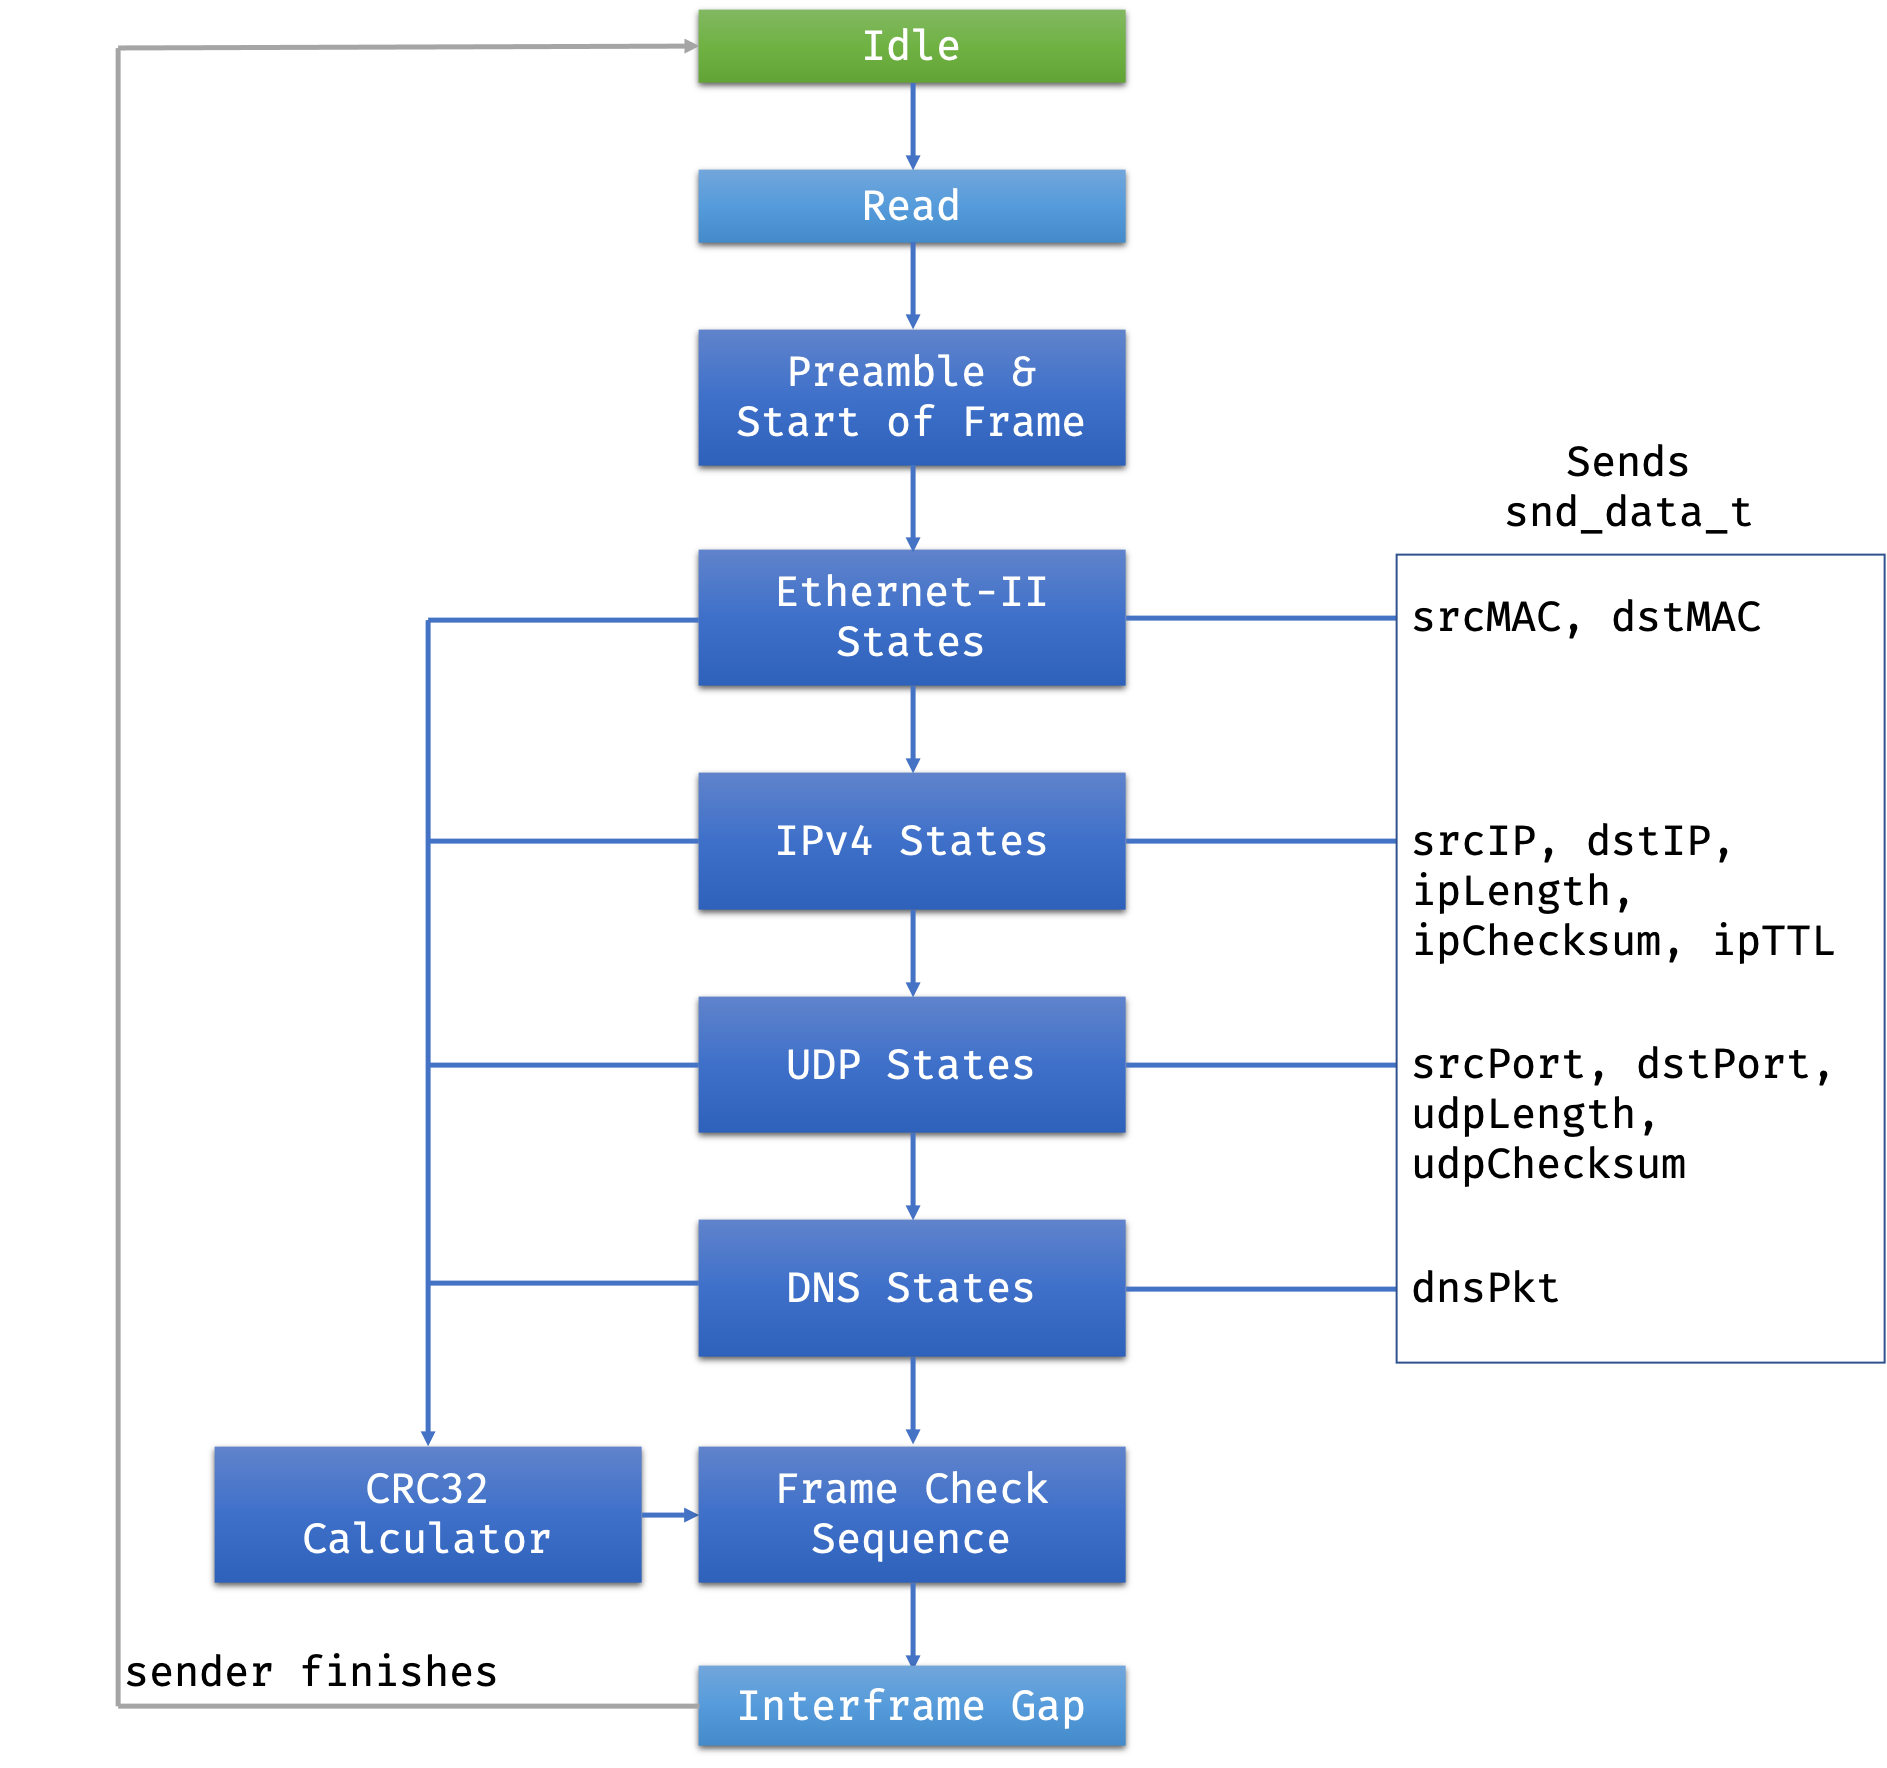
\includegraphics[width=0.8\textwidth]{imgs/snd-fsm.png}}
  \caption{\code{mac\_snd.vhd} Module FSM Overview}
  \label{fig:snd-fsm}
\end{figure}

Similarly, we also implemented the Sender interfacing with the PHY transmitter with an FSM shown in Figure \ref{fig:snd-fsm}. While the internal logic is in reverse order, sending signals to the interfaces rather than receiving, the general states of the FSM are alike. Note that the sender operates based on a sending struct named \code{snd\_data\_t} with checksums and TTLs calculated and metadata imported from previous steps at state \code{Read}. As the sender pulls up \code{TX\_EN} and sends nibble streams to the \code{TXD} interface, the CRC32 calculator also receives the stream and calculates the next-state FSM within the clock cycle. When all the DNS payload has been transmitted, the 32-bit (8-byte) CRC sequence will be emitted by the calculator component and appended to the packet. Lastly, but easily forgotten, Ethernet-II requires an inter-frame gap of 12 octets (24 nibbles) of \code{TX\_EN} at GND before a new packet can be transmitted. Not following the procedure properly would cause the next packet to be discarded by the intended recipients.

\subsection{Clock-Domain-Crossing FIFO}

One of the most common methods of transferring data across clock domains is to use a FIFO buffer. In a hardware implementation, a CDC FIFO is usually a dual-port RAM that operates separately with a read CLK and a write CLK. In our CDC FIFO design shown in Listing \ref{lst:fifo-rcv-vhd}, we introduce two pairs of behavioural circuits corresponding to reading and writing to the FIFO. Each pair consists of a Next-State-Logic (NSL), which detects and operates read and write on the FIFO, and a register (REG) process that updates the index pointer state of the FIFO. Whenever there is a packet left to be processed in the FIFO, the \code{buf\_not\_empty} signal would be pulled to VCC in order to make the predecessor aware of the new task at hand.

\begin{lstlisting}[language=VHDL, caption=Snippet of FIFO \code{FIFO\_receive.vhd}, label={lst:fifo-rcv-vhd}]
  fifo_wnsl : PROCESS (wclk)
  BEGIN
    IF (rising_edge(wclk)) THEN IF (w_en = '1') THEN
      ... ELSE ...
    END IF; END IF;
  END PROCESS;

  fifo_wreg : PROCESS (wclk)
  BEGIN
    IF falling_edge(wclk) THEN
      w_index <= win_index;
    END IF;
  END PROCESS;

  fifo_rnsl : PROCESS (rclk)
  BEGIN
    IF (rising_edge(rclk)) THEN IF (r_en = '1') THEN
        ... ELSE ...
    END IF; END IF;
  END PROCESS;

  fifo_rreg : PROCESS (rclk)
  BEGIN
    IF falling_edge(rclk) THEN
      r_index <= rin_index;
    END IF;
  END PROCESS;

  buf_not_empty <= '0' WHEN w_index = r_index ELSE '1';
\end{lstlisting}

We omit the commonly used Almost Full (AF) and Almost Empty (AE) flags in our FIFO as an implementation decision to discard all eight packets left unprocessed within the FIFO when index pointers collide, meaning the FIFO is full and unable to receive new packets. This is unlikely to happen as the core operates at a much higher speed with two times lower processing time than the PHY clock domain. Hence, it is almost impossible to flood the core with too many packets to process. On rare occasions it does happen; however, there would be no difference in discarding new incoming packets or current packets in the FIFO as they are of equal importance. This also omits extra logic to check and monitor the FIFO status, yielding minor latency improvements to the design.

\subsection{Core Input Processor}

\begin{figure}[h!]
  \makebox[\textwidth][c]{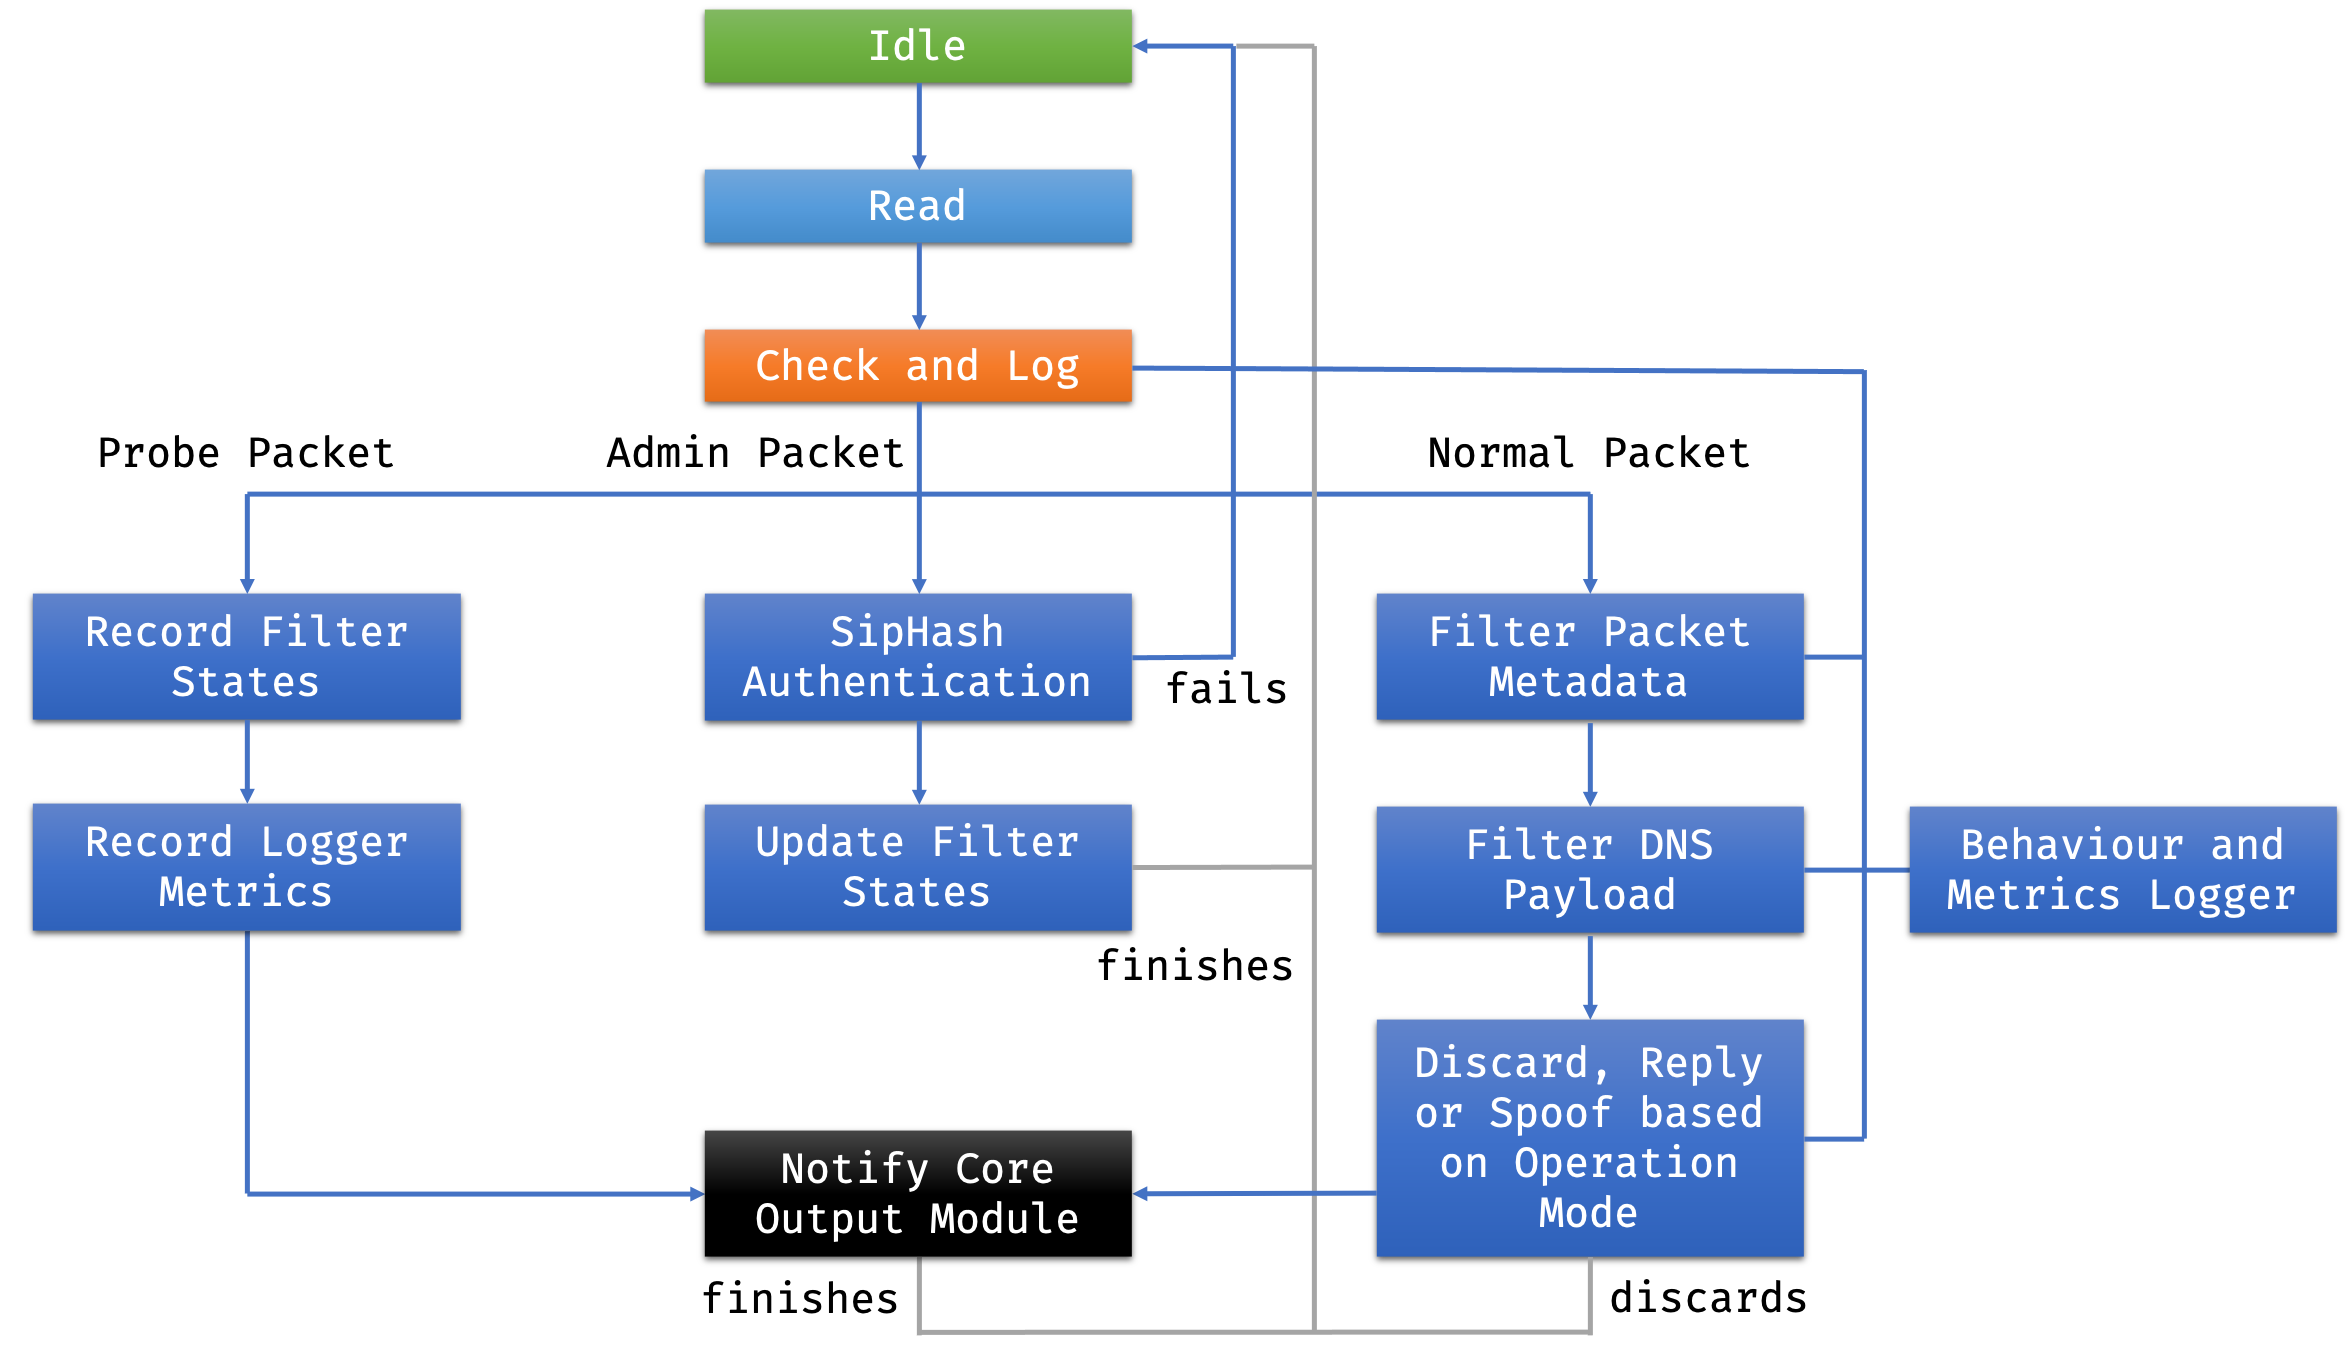
\includegraphics[width=\textwidth]{imgs/corein-fsm.png}}
  \caption{\code{i.vhd} Module FSM Overview}
  \label{fig:corein-fsm}
\end{figure}

The Core Input Processor is where the core processing and handling of network packets happens. Its high-level FSM is demonstrated in Figure \ref{fig:corein-fsm}. As the FIFO signals the \code{corein} unit, the full packet struct of \code{rcv\_data\_t} will be fetched at the \code{Read} state. The processor will then log the packet and identify the packet into three main categories:
\begin{itemize}
    \item Probe Packet: Packet that probes the FPGA for its current configuration and up-to-date metrics.
    \item Admin Packet: Packet sent from the FPGA administrators that carry new information for filters and operation mode configurations.
    \item Normal Network Packet: Packet that shall be checked and acted upon based on current on-board filter and operation configurations.
\end{itemize}

For a regular network packet received, it will be filtered/checked in the areas of MAC addresses, IP addresses, UDP ports, DNS headers and domain names. The filter will compare this information to given lists in the configuration. Dependent on the lists being blacklists or whitelists, the processor will provide a binary decision at the end of each procedure. By the end of all checks, the checkers will reach a final binary decision of pass or not pass. Based on the FPGA operation mode (man-in-the-middle filter mode, man-on-the-side spoof mode), the FPGA will take one of the four actions as instructed: forward the payload, forward the DNS transaction, spoof a DNS transaction or discard the packet. Depending on the result, the core output module will be notified accordingly to deal with packet checksums and other relevant metadata. This is estimated to take at least $10$ clock cycles ($200\; ns$) under the best cases and at most $120$ clock cycles ($2400\; ns$) with the largest payload bounded by the packet length limitation, and the most complex filters.  

Once a probe packet is logged, the FPGA will pack the current filter configurations and logger metrics by bits in a compact packet and pass them on to the core output constructor for checksum calculations in less than 20 clock cycles (400 ns); relatively quick and straightforward.

Since an attacker can potentially disable the FPGA system via an admin packet, extra authentication is needed for the FPGA to recognise legitimate administration updates. The FPGA uses SipHash\footnote{See Section \ref{section:implementation-hardware-implementation-siphash} for more information about SipHash authentication} to validate the 64-bit MAC appended to the admin payload. Once it is verified, the FPGA will then update filter configurations and reset loggers and the system as instructed. Given the enhanced security on this section of the sequential circuit, it is expected to cost around 400 clock cycles (8000 ns) for a full filter update, and a logger reset. This is acceptable even for latency-sensitive use cases as updating filters could be rather rare, and there are no reply actions needed afterwards.

If a packet needs to be sent after the procedure, the processor shall pull up \code{snd\_en}, and the Core Output Constructor will be notified to deal with the heavy lifting of checksums and size calculations.

\subsection{SipHash Authentication Component}
\label{section:implementation-hardware-implementation-siphash}

\begin{figure}[h!]
\centering
\begin{minipage}{.45\textwidth}
  \makebox[\textwidth][c]{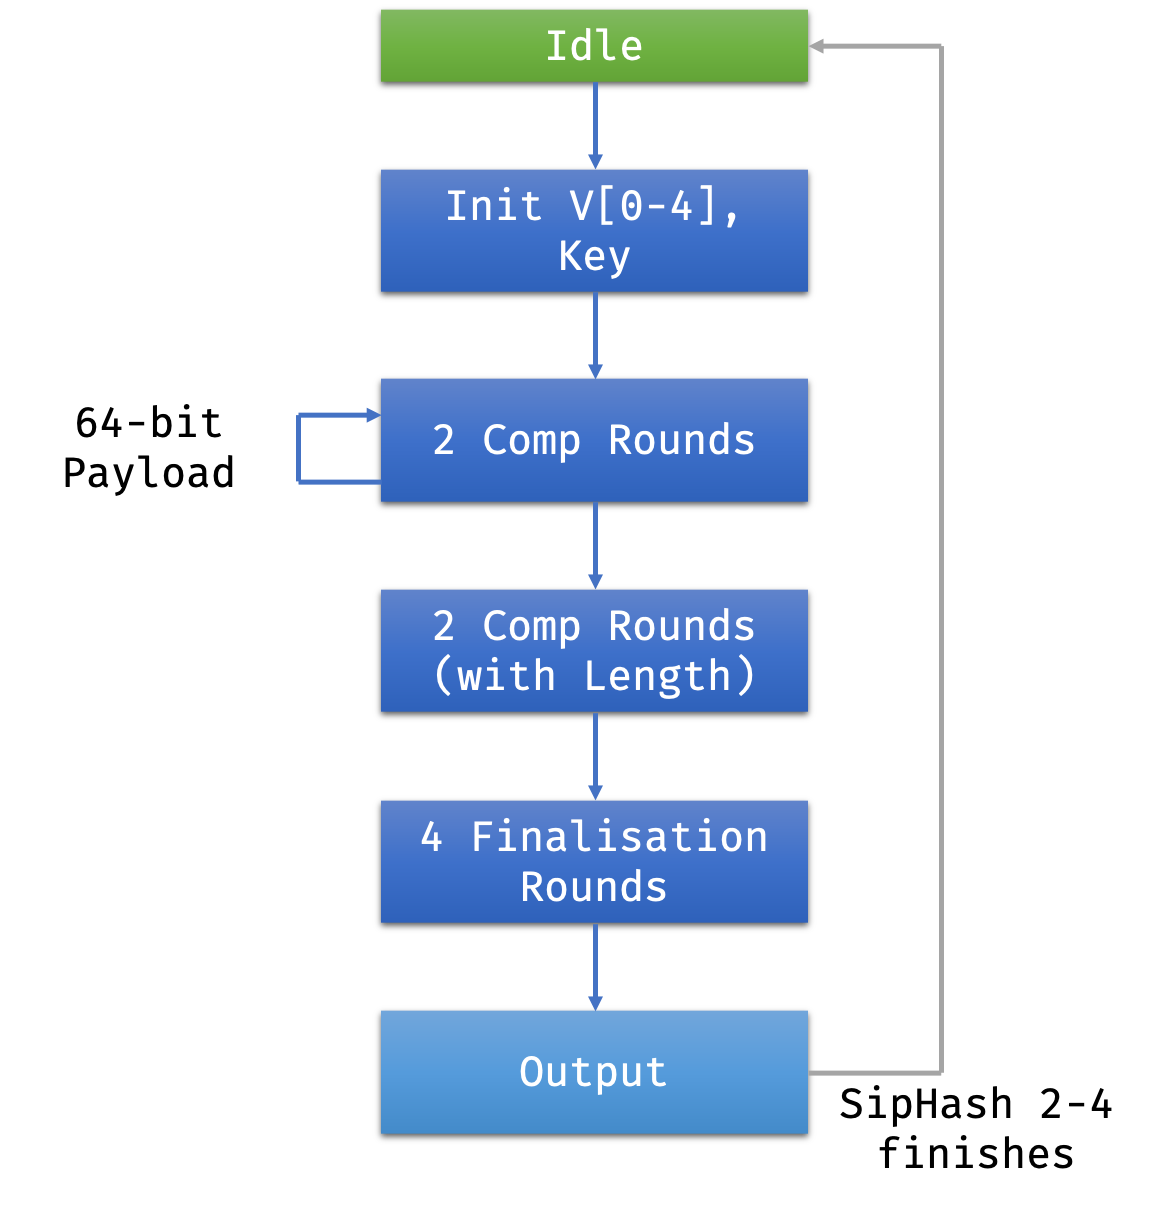
\includegraphics[width=\textwidth]{imgs/siphasher-fsm.png}}
  \caption{\code{siphasher.vhd} Module FSM Overview}
  \label{fig:siphasher-fsm}
\end{minipage}
\begin{minipage}{.45\textwidth}
  \makebox[\textwidth][c]{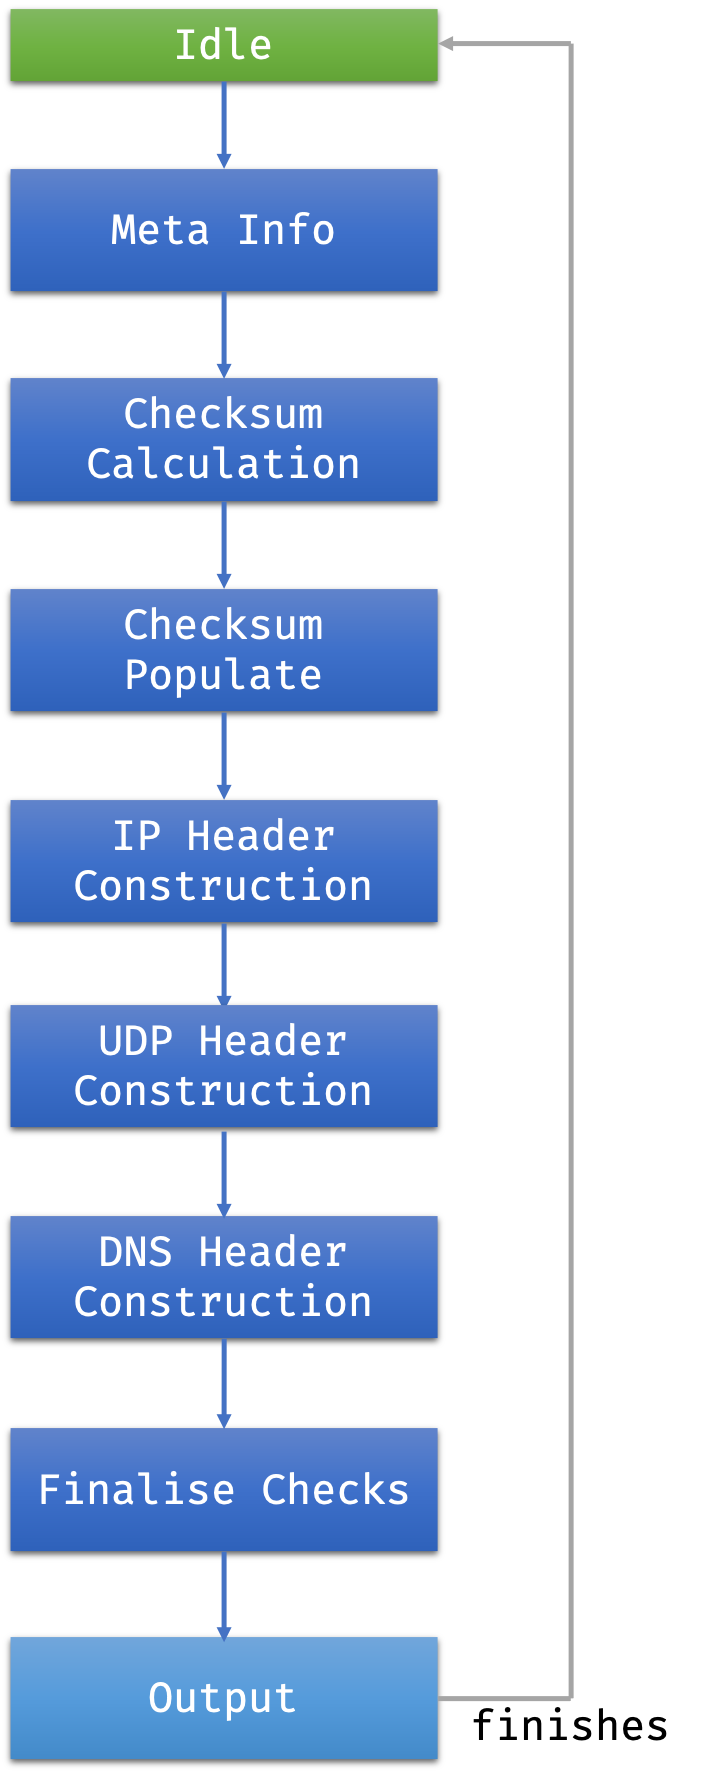
\includegraphics[width=0.6\textwidth]{imgs/coreout-fsm.png}}
  \caption{\code{o.vhd} Module FSM Overview}
  \label{fig:coreout-fsm}
\end{minipage}
\end{figure}

Given the complexity of SipHash calculations, we implemented a separate hardware component for this purpose. Across multiple variants of hash algorithms in the SipHash family, we adopted SipHash 2-4 in favour of its simplicity and speed. From the paper by Jean-Philippe Aumasson \cite{aumasson-bernstein-2012}, SipHash 2-4 process is comprised of a key round, 2 compression rounds on every 64 bits of the payload, 2 compression rounds on the payload length and 4 finalising rounds. Each round involves the same set of obfuscation rounds known as SipRounds.

Therefore, given the steps, we implemented the \code{siphasher} unit with the FSM shown in Figure \ref{fig:siphasher-fsm}. The 1024-bit (128-byte) payload of the admin packet is allocated with 960 bits (120 bytes) of payload and 64 bits (8 bytes) of MAC. Before the admin packet acknowledgement, the output of \code{siphasher} will be checked against the final 64 bits (8 bytes) in the payload to confirm the admin information's validity. The SipHash key in hardware shall be edited in the \proglang{VHDL} module before synthesis and implementation and will be hardcoded into the FPGA core. This key shall be identical to the one used in the software control system. Otherwise, the hardware would deem the admin packet invalid and log the malicious behaviour of faking an administrator.

\subsection{Core Output Packet Constructor}

The final key component within the hardware implementation is the Core Output Packet Constructor \code{coreout}. This component is a sequential circuit that handles the struct transition from \code{rcv\_data\_t} to \code{snd\_data\_t}, while populating certain fields including sizes and checksums. The FSM overview containing construction steps can be viewed in Figure \ref{fig:coreout-fsm}. The current version of \code{coreout} would only compute the IPv4 checksum and discard UDP checksums by default for latency reasons. The whole streamlined process takes less than $10$ clock cycles ($200\; ns$) until the packet is on its way to the sender FIFO queuing to be sent to the MII interface.


\section{Hardware Pitfalls \& Debugging}
\label{section:implementation-hardware-debugging}

This section describes all the pitfalls and challenges we met, investigated and eventually overcame during the project development process. This was a tirelessly grinding process with more than 600 hours spent. All code listings below are minimised actual code snippets from HDL source files within the project. 

\subsection{HDL Pitfalls - Timing and Execution Models}

\begin{minipage}{.45\textwidth}
\begin{lstlisting}[language=VHDL, caption=Faulty Signal Update in \proglang{VHDL}, label={lst:faulty-signal-update}]
SIGNAL s : STD_LOGIC;

proc : PROCESS (clk)
BEGIN
  IF (rising_edge(clk)) THEN
    s <= '1';
    IF (s = '1') THEN
    ... ELSE ...
    END IF;
  END IF;
END PROCESS;
\end{lstlisting}
\end{minipage}\hfill
\begin{minipage}{.45\textwidth}
\begin{lstlisting}[language=VHDL, caption=Correct Signal Update in \proglang{VHDL}, label={lst:correct-signal-update}]
SIGNAL s, sin : STD_LOGIC;

proc : PROCESS (clk)
BEGIN
  IF (rising_edge(clk)) THEN
    sin <= '1';
    IF (s = '1') THEN
    ... ELSE ...
    END IF;
  END IF;
END PROCESS;

reg : PROCESS (clk)
BEGIN
  IF (falling_edge(clk)) THEN
    s <= sin;
  END IF;
END PROCESS;
\end{lstlisting}
\end{minipage}

At first glance, building hardware with HDL seems to be very similar to engineering software with a programming language, not to mention that \proglang{VHDL} has a close resemblance to \proglang{Ada} while \proglang{Verilog} and \proglang{C} are pretty much alike. However, they are fundamentally different as HDL aims to describe static computing models with the explicit notion of concept ``time", albeit concurrent or sequential, while software languages aim to produce a list of instructions that execute in order. That is why HDLs resembles specific concurrent programming languages in their ability to model parallel processes that execute continuously independently of one another.

It is crucial to understand the timing model and promises of an HDL before we program a component. We initially implemented the faulty signal update logic as shown in Listing \ref{lst:faulty-signal-update}. From a software perspective, it would be perfectly valid to update \code{s}, reading it later on in a sequential statement. However, \code{VHDL}'s time model assumes that a signal change does not happen immediately but is scheduled at the end of the current process delta cycle. That is to say, signal \code{s} will not be updated until all executing processes have ended. This is a common pitfall when implementing hardware in \proglang{VHDL} and can be tough to spot in complicated branching statements. Thus, as shown in Listing \ref{lst:correct-signal-update} and previous FSM Listing \ref{lst:one-hot-fsm-minimal}, we would design a current state signal \code{s} to read from and a next state signal \code{sin} to write to within a process, and explicitly update \code{s} \textleftarrow \code{sin} after delay upon a falling clock edge. 

\begin{lstlisting}[language=VHDL, caption=Faulty Unrolled Loop Sample in \proglang{VHDL}, label={lst:unrolled-loop}]
proc : PROCESS (clk)
VARIABLE d : STD_LOGIC_VECTOR(255 DOWNTO 0) := (OTHERS => '0');
VARIABLE c : NATURAL RANGE 0 TO 255;
BEGIN
  IF (rising_edge(clk)) THEN
    FOR i IN 0 TO 255 LOOP
      IF (d(i) = '1') THEN
        c := c + 1;
      END IF;
    END LOOP;
    ... 
  END IF;
END PROCESS;
\end{lstlisting}

To allow direct usage after assignment within the same clock cycle / single activation, we can introduce variables in \proglang{VHDL} that have a different timing promise according to the model. While signals are usually actual flip flops with persistent data stored, variables can be seen as temporary design objects that store middle states. Hence, we made another mistake of abusing loops and variables usages in a single clock cycle, listed in Listing \ref{lst:unrolled-loop}. It would be common from a software perspective to believe that the loop would execute one iteration per clock cycle. Instead, the synthesiser would unroll the loop entirely and generate enough hardware to execute all iterations in parallel. Hence, we are effectively producing a circuit where the variable \code{c} gets incremented $0$-$255$ times at the same clock cycle within $20$ns. The implementation could only be possible when the data width of \code{d} is minimal, and the branches are extremely short. Otherwise, it would be impossible for the router to find an implementation within the timing constraint\footnote{See Section \ref{section:implementation-hardware-implementation-timing} for more information about timing constraints}.

\subsection{HDL Pitfalls - Simulation and Implementation Difference}
\label{section:implementation-hardware-debugging-hdl-pitfalls-simulation-and-implementation}

\begin{lstlisting}[language=VHDL, caption=Faulty \code{STD\_LOGIC\_VECTOR} comparison in \proglang{VHDL}, label={lst:faulty-comparison}]
IF (rd.dnsPkt(DOMAIN_LENGTH + OFFSET DOWNTO OFFSET)
  = f.dnsList(FILTER_INDEX)(DOMAIN_LENGTH DOWNTO 0)) THEN
  ...
END IF;
\end{lstlisting}

Besides the pitfalls above, HDLs themselves include certain subsets within the language aimed at writing verification code (i.e. test benches) instead of a circuit in hardware. One very subtle error we countered during the development can be attributed to this cause. When comparing domain names with DNS payload in hardware, we designed our component to follow the HDL shown in Listing \ref{lst:faulty-comparison}. The code simply compares a portion in the DNS payload from \code{OFFSET} to \code{DOMAIN\_LENGTH + OFFSET}, with the \code{FILTER\_INDEX} string in the filter of the same width.

This piece of code worked well within the \code{xsim} simulator and produced correct results when the domain names match an item in the filter list on behavioural simulation. However, when we later implemented the design in hardware, none of the packets were recognised and filtered successfully. Nevertheless, the synthesiser, router and bitstream generator produces no warning nor error related to this component, which seems unreasonable. Upon further investigation and reading language specs, we realised that the synthesiser would not be able to produce the electrical component for a variable width comparison in hardware. Instead, it would simply resort to the longest possible comparison that
is viable for both sides. In this case, as the \code{dnsPkt} is longer than \code{f.dnsList(FILTER\_INDEX)}, it would compare the packet payload with the entire \code{f.dnsList}, regardless of the later specified range.

\begin{lstlisting}[language=VHDL, caption=Dynamic width \code{STD\_LOGIC\_VECTOR} comparison in \proglang{VHDL}, label={lst:correct-comparison}]
  IF (s.fpktc >= 32) THEN       -- 4 bytes
    IF (rd.dnsPkt((s.fpktsc + s.fpktc - 1) DOWNTO (s.fpktsc + s.fpktc - 32))
      = f.dnsList(s.fdnsc)((s.fpktc - 1) DOWNTO (s.fpktc - 32))) THEN
    ... ELSE ...
    END IF;
  ELSIF (s.fpktc >= 24) THEN    -- 3 bytes
    IF (rd.dnsPkt((s.fpktsc + s.fpktc - 1) DOWNTO (s.fpktsc + s.fpktc - 24))
      = f.dnsList(s.fdnsc)((s.fpktc - 1) DOWNTO (s.fpktc - 24))) THEN
    ... ELSE ...
    END IF;          
  ELSIF (s.fpktc >= 16) THEN    -- 2 bytes    
    IF (rd.dnsPkt((s.fpktsc + s.fpktc - 1) DOWNTO (s.fpktsc + s.fpktc - 16))
      = f.dnsList(s.fdnsc)((s.fpktc - 1) DOWNTO (s.fpktc - 16))) THEN
    ... ELSE ...
    END IF;                 
  ELSIF (s.fpktc >= 8) THEN     -- 1 byte
    IF (rd.dnsPkt((s.fpktsc + s.fpktc - 1) DOWNTO (s.fpktsc + s.fpktc - 8))
      = f.dnsList(s.fdnsc)((s.fpktc - 1) DOWNTO (s.fpktc - 8))) THEN
    ... ELSE ...
    END IF;
  ELSE
    ...
  END IF; 
\end{lstlisting}

Hence, we needed to eliminate all dynamic width comparisons within the code to work around this issue. One alternative is to compare $n$ bytes at a time until there are less than $n$ bytes left. At a later clock cycle, we would generate all $0 \;...\;n-1$ byte comparison to deal with the modulus. The minimised code structure can be seen at Listing \ref{lst:correct-comparison}. With that approach, we would be able to pass both behavioural simulation and post-implementation hardware simulation. However, as it finally turns out, this solution would impose too strict timing on the wire placement and enough load on the driving signals to cause metastability and fail timing constraints\footnote{See Section \ref{section:implementation-hardware-implementation-metastability} and \ref{section:implementation-hardware-implementation-timing} for more information on signal metastability and timing constraints}. Further pipelining is required to make the filter work properly in hardware.

\subsection{Timing Pitfalls - Clock Domain Crossing and Signal Metastability}
\label{section:implementation-hardware-implementation-metastability}

\begin{figure}[h!]
  \makebox[\textwidth][c]{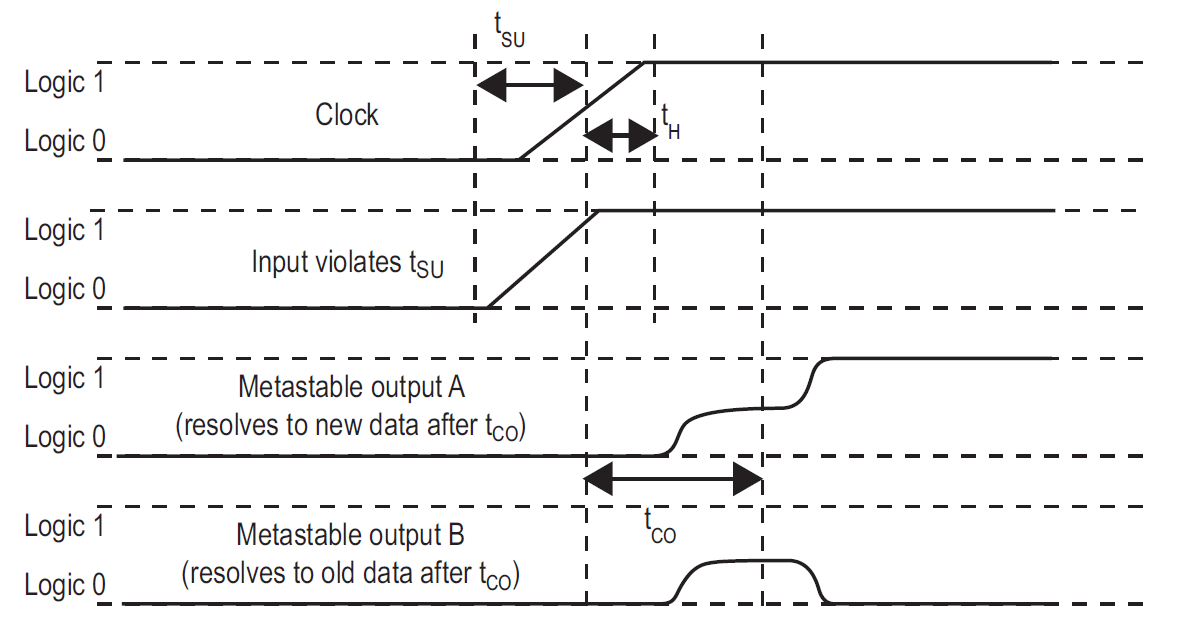
\includegraphics[width=\textwidth, height=0.45\textwidth]{imgs/metastability-clock.png}}
  \caption{Metastable sample signal graph \cite{stephenson-2009}}
  \label{fig:metastability-clock}
\end{figure}

Metastability describes a phenomenon where an electronic element persists for an unbounded amount of time in an unstable (metastable) state \cite{chaney-1973}. It causes digital systems to fail and exhibit indeterminate behaviour, which is troublesome to debug and fix. To explain why metastability happens, we need to elaborate on how a signal transverse throughout a digital system. All FPGA components have defined timing requirements that allow each register to receive input and produce output signals. To guarantee reliable operation, it is necessary to hold the input for a minimum register setup time $t_{SU}$ before the clock edge, and a minimum hold time after the clock edge $t_{H}$. The register output becomes available after a clock-to-output delay $t_{CO}$. If either $t_{SU}$ or $t_{H}$ is violated, we will then receive output signals in a so-called metastable state. To elaborate, the output signal could hover at any instant between VCC and GND for a random amount of time even after the previously guaranteed $t_{CO}$, as shown in Figure \ref{fig:metastability-clock}. In the end, the signal can either resolve to high or low or even keep in the middle as an undefined signal. The signal transition through the register is analogous to balancing a ball at the top of the hill, as demonstrated in Figure \ref{fig:metastability-analogy}.

\begin{figure}[h!]
  \makebox[\textwidth][c]{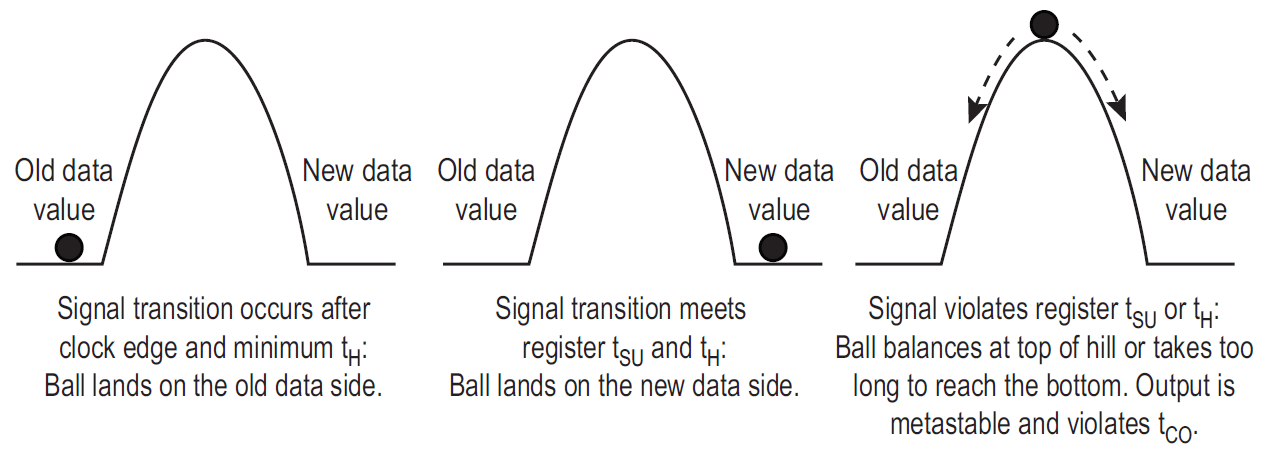
\includegraphics[width=\textwidth, height=0.3\textwidth]{imgs/metastability-analogy.png}}
  \caption{Metastable signal analogy \cite{stephenson-2009}}
  \label{fig:metastability-analogy}
\end{figure}

As mentioned previously in Section \ref{section:implementation-hardware-implementation-top-level-clock-divdier}, the design features two clock domains, one for the PHY and MAC sender and receiver peripheral, and the other one for the FPGA core processor. As packet signals are crossing clock boundaries, the transition can happen at any point relative to the receiving clock edge of the capturing unit. Hence, the designer would be unable to predict the sequence of signals transmitted or the number of destination clock edges until the data finishes transmitting. As a result, the received values could very likely be incorrect and result in unexpected behaviour within the circuit. 
 
We were initially unaware of the CDC metastability issue and experienced unpredictable cases of packet loss and disappearance in the middle of the process. Later, the issue was relieved when we throttled the processing core down to $25$ MHz and used the same reference clock as the PHY peripherals. This is not ideal as we could have achieved two times faster speed with the processing.

\begin{figure}[h!]
  \makebox[\textwidth][c]{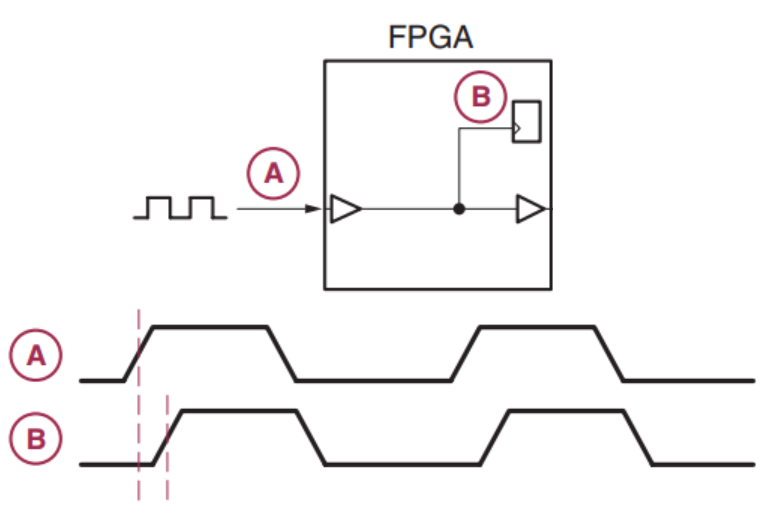
\includegraphics[width=0.36\textwidth]{imgs/clock-skew.png}}
  \caption{Clock Skew demonstration \cite{arar-2018}}
  \label{fig:clock-skew}
\end{figure}

One might argue that the PHY reference clock is generated by the clock divider within the design, as specified in Section \ref{section:implementation-hardware-implementation-top-level-clock-divdier}; hence the design should be synchronous, and the timing requirements should be predictable. However, this is unfortunately not the case. Although the clock division shall be reasonably straightforward, it still takes a tiny portion of time and imposes a $\Delta t$ delay (skew) on the generated clocks, demonstrated in Figure \ref{fig:clock-skew}. The reference clock would then be provided to the PHY chip peripheral, while the design operates on the PHY feedback clock \code{E\_RX\_CLK} and \code{E\_TX\_CLK}. Thus, the PHY chip would also append an unknown amount of skew to the \code{E\_REF\_CLK}. In total, there is a 2-skew delay and 1:4 division from the original oscillator clock. Moreover, internal clocks go through an isolated fast path named the clock path, hypersensitive to delays and skews. Thus, routing the significantly skewed PHY clock through the fast clock paths in FPGA is infeasible, as it would cause a substantial number of timing errors across the core circuit. Consequently, it is a hardware-implementation decision to make the system an asynchronous design, resulting in vulnerability to CDC and metastability issues.
 
As explained in design Section \ref{section:design-system-design-hardware}: dual-clock FIFO (DCFIFO) is later designed and implemented in hardware to store the middle signal states, guaranteeing timing requirements. Also, multiple handshaking logic signals, including \code{DV}, \code{EN} and \code{ACK} are in place to further assure successful recognition of these CDC signals.

\subsection{Timing Pitfalls - Unintended Inferred Latches}

In this section, we will be referring to FFs exclusively as edge-triggered (synchronous) flip flops. Level-triggered (asynchronous) storage units are referred to as latches for clarification.

In most FPGA designs, FFs are used commonly across most FPGA designs as the basic storage unit. On the other hand, latches are rare in FPGA designs but more common in ASICs suited to mainframes and supercomputers \cite{vasumathi-2018}. Latches deployed properly can improve machine cycle time in systems where the clock skew is a substantial fraction of the total clock cycle time \cite{vasumathi-2018}. However, in FPGAs, latches are very poor matches as their main benefit is almost non-existent in such a small chip where its clock distribution skew is effectively zero.

\begin{minipage}{.45\textwidth}
\begin{lstlisting}[language=VHDL, caption=Inferred Latch with missing branch in \proglang{VHDL}, label={lst:inferred-latch-missing-branch}]
IF (R_EN = '1') THEN
  out_d <= in_d;
END IF;
\end{lstlisting}
\end{minipage}\hfill
\begin{minipage}{.45\textwidth}
\begin{lstlisting}[language=VHDL, caption=Inferred Latch with incomplete assignment, label={lst:non-inferred-latch}]
-- default assignment 
out_d <= (OTHERS => '0');
IF (R_EN = '1') THEN
  out_d <= in_d;
END IF;

-- ELSE statement
IF (R_EN = '1') THEN
  out_d <= in_d;
ELSE
  out_d <= (OTHERS => '0');
END IF;
\end{lstlisting}
\end{minipage}

Latches are inferred in \proglang{VHDL} code primarily due to the language's guarantee when encountering unassigned signals. As shown in Listing \ref{lst:inferred-latch-missing-branch}, the \code{IF} statement sets \code{out\_d} to \code{in\_d} on branch, but does not specify what it shall be when not enabled. In this case, \proglang{VHDL} guarantees that the original value of \code{out\_d} would remain unchanged, hence a latch is inferred to preserve the original \code{out\_d} value. To avoid inferring a latch here, we shall append an \code{ELSE} statement before the \code{END IF} statement or specify a default assignment before the \code{IF} statement, as shown in Listing \ref{lst:non-inferred-latch}.

\begin{lstlisting}[language=VHDL, caption=An sample latch set on packet counter reaching $\mathtt{0x100}$, label={lst:sample-latch-issue}]
latch_en <= '1' WHEN packet_count = x"100" ELSE '0';
\end{lstlisting}

Given the asynchronous nature of latches, it can cause not only metastability issues as detailed in the previous Section \ref{section:implementation-hardware-implementation-metastability}, but also worse failures based on hardware implementation details. For example, we can infer a latch that is enabled every time upon packet counter reaching $\mathtt{0x100}$, regardless of the clock, with the code shown in Listing \ref{lst:sample-latch-issue}. This seems fine as a purely combinatorial logic comprised of several gates and LUTs. However, the signal paths from \code{packet\_count} to \code{latch\_en} would never be perfect, and there could be occasional glitches on it. For instance, imagine \code{packet\_count} is has not yet reached $\mathtt{0x100}$, but due to a signal path to \code{latch\_en} being marginally longer than the other route at an XOR-gate, \code{latch\_en} can go to VCC for an instant before settling down to GND, within its clock-to-output delay $t_{co}$. If it were an FF here, no issue will be caused as the FF would be clocked to wait for the next rising edge to update its internal value, which is far away at this point in time. Unfortunately, given a latch here, the unintended value will be sent mistakenly. Making it worse, if the logic paths for the \code{latch\_en} signal were routed slightly differently (with different amount of delays), then the glitch behaviour would also change. It might work just fine in the design until something else completely unrelated changes and the fitter routes the whole design differently on the FPGA, causing the failure to happen. This brought great uncertainty to the development, since failures appear completely random. During the project, this happened on several occasions where weeks were spent just to figure out a single unneeded latch causing these types of problems.

\begin{figure}[h!]
  \makebox[\textwidth][c]{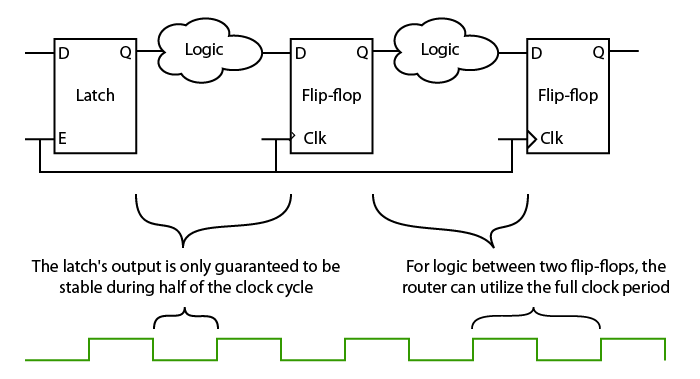
\includegraphics[width=0.6\textwidth]{imgs/latch-timing.png}}
  \caption{Latch strict timing requirements \cite{jensen-2020}}
  \label{fig:latch-timing}
\end{figure}

Last, but not least, using latches also imposes stricter timing requirements on the placer and router. As shown in Figure \ref{fig:latch-timing}, the left-hand side of the Figure illustrates a signal traversing from a latch to a FF. Since the latch only guarantees stability during the lower half of the cycle, the logic depth is heavily restricted as we could waste the entire clock VCC period waiting for a latch to be stable. Instead, when traversing from a FF to another one, the router can utilise the entire clock period as FFs would only change upon a rising clock edge.

In all, we have thoroughly analysed the timing pitfalls caused by implicitly inferring latches within the design. The main takeaway that we had throughout the debugging process is the in-depth understanding of why all sorts of issues happen with latches in the FPGA and to avoid latches unless strictly necessary in all future designs.

\subsection{Timing Pitfalls - Pipelining and Strict Timing Constraints}
\label{section:implementation-hardware-implementation-timing}

\begin{figure}[h!]
  \makebox[\textwidth][c]{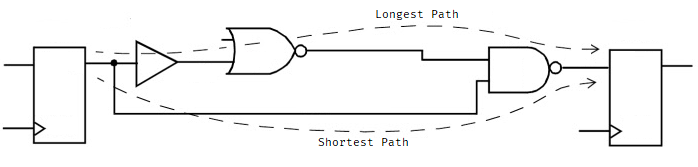
\includegraphics[width=\textwidth]{imgs/timing-path.png}}
  \caption{Signal Propagation paths within a clock cycle from a source FF to a destination FF}
  \label{fig:timing-path}
\end{figure}

As hardware circuits execute, electrical signals would be required to traverse through multiple logic gates, within a clock cycle, from a source register to a destination register. Upon traversing through each logic gate, a tiny portion of time is taken to produce a stable output, called the gate delay. In a synchronous digital system, signals are regulated to move in lockstep, advancing one stage on each tick of the clock. This is usually enforced by synchronising endpoint registers (FFS), which forward the input signal to output on a rising edge. The number of gates throughout a specific path is called its logic depth. Due to technical limitations, most circuit designs cannot guarantee that all paths are created with the exact same logic depth, as demonstrated in Figure \ref{fig:timing-path}. This creates a very much undesired timing difference in the propagation delays across different paths, which is the major contributor to various glitches resulting from race conditions. In synchronous circuits specifically, the propagation time difference might also cause register timing violations in two different ways:

\begin{itemize}
    \item Maximum time violation: when the path logic is too deep that the signal would arrive too late at the receiving FF and miss the setup time of the register $t_{SU}$.
    \item Minimum time violation: when the path logic is not long enough, the signal changes too soon after the clock's state transition. The receive FF would not have enough hold time $t_{H}$ for the input signal to register properly.
\end{itemize}

\begin{figure}[h!]
  \makebox[\textwidth][c]{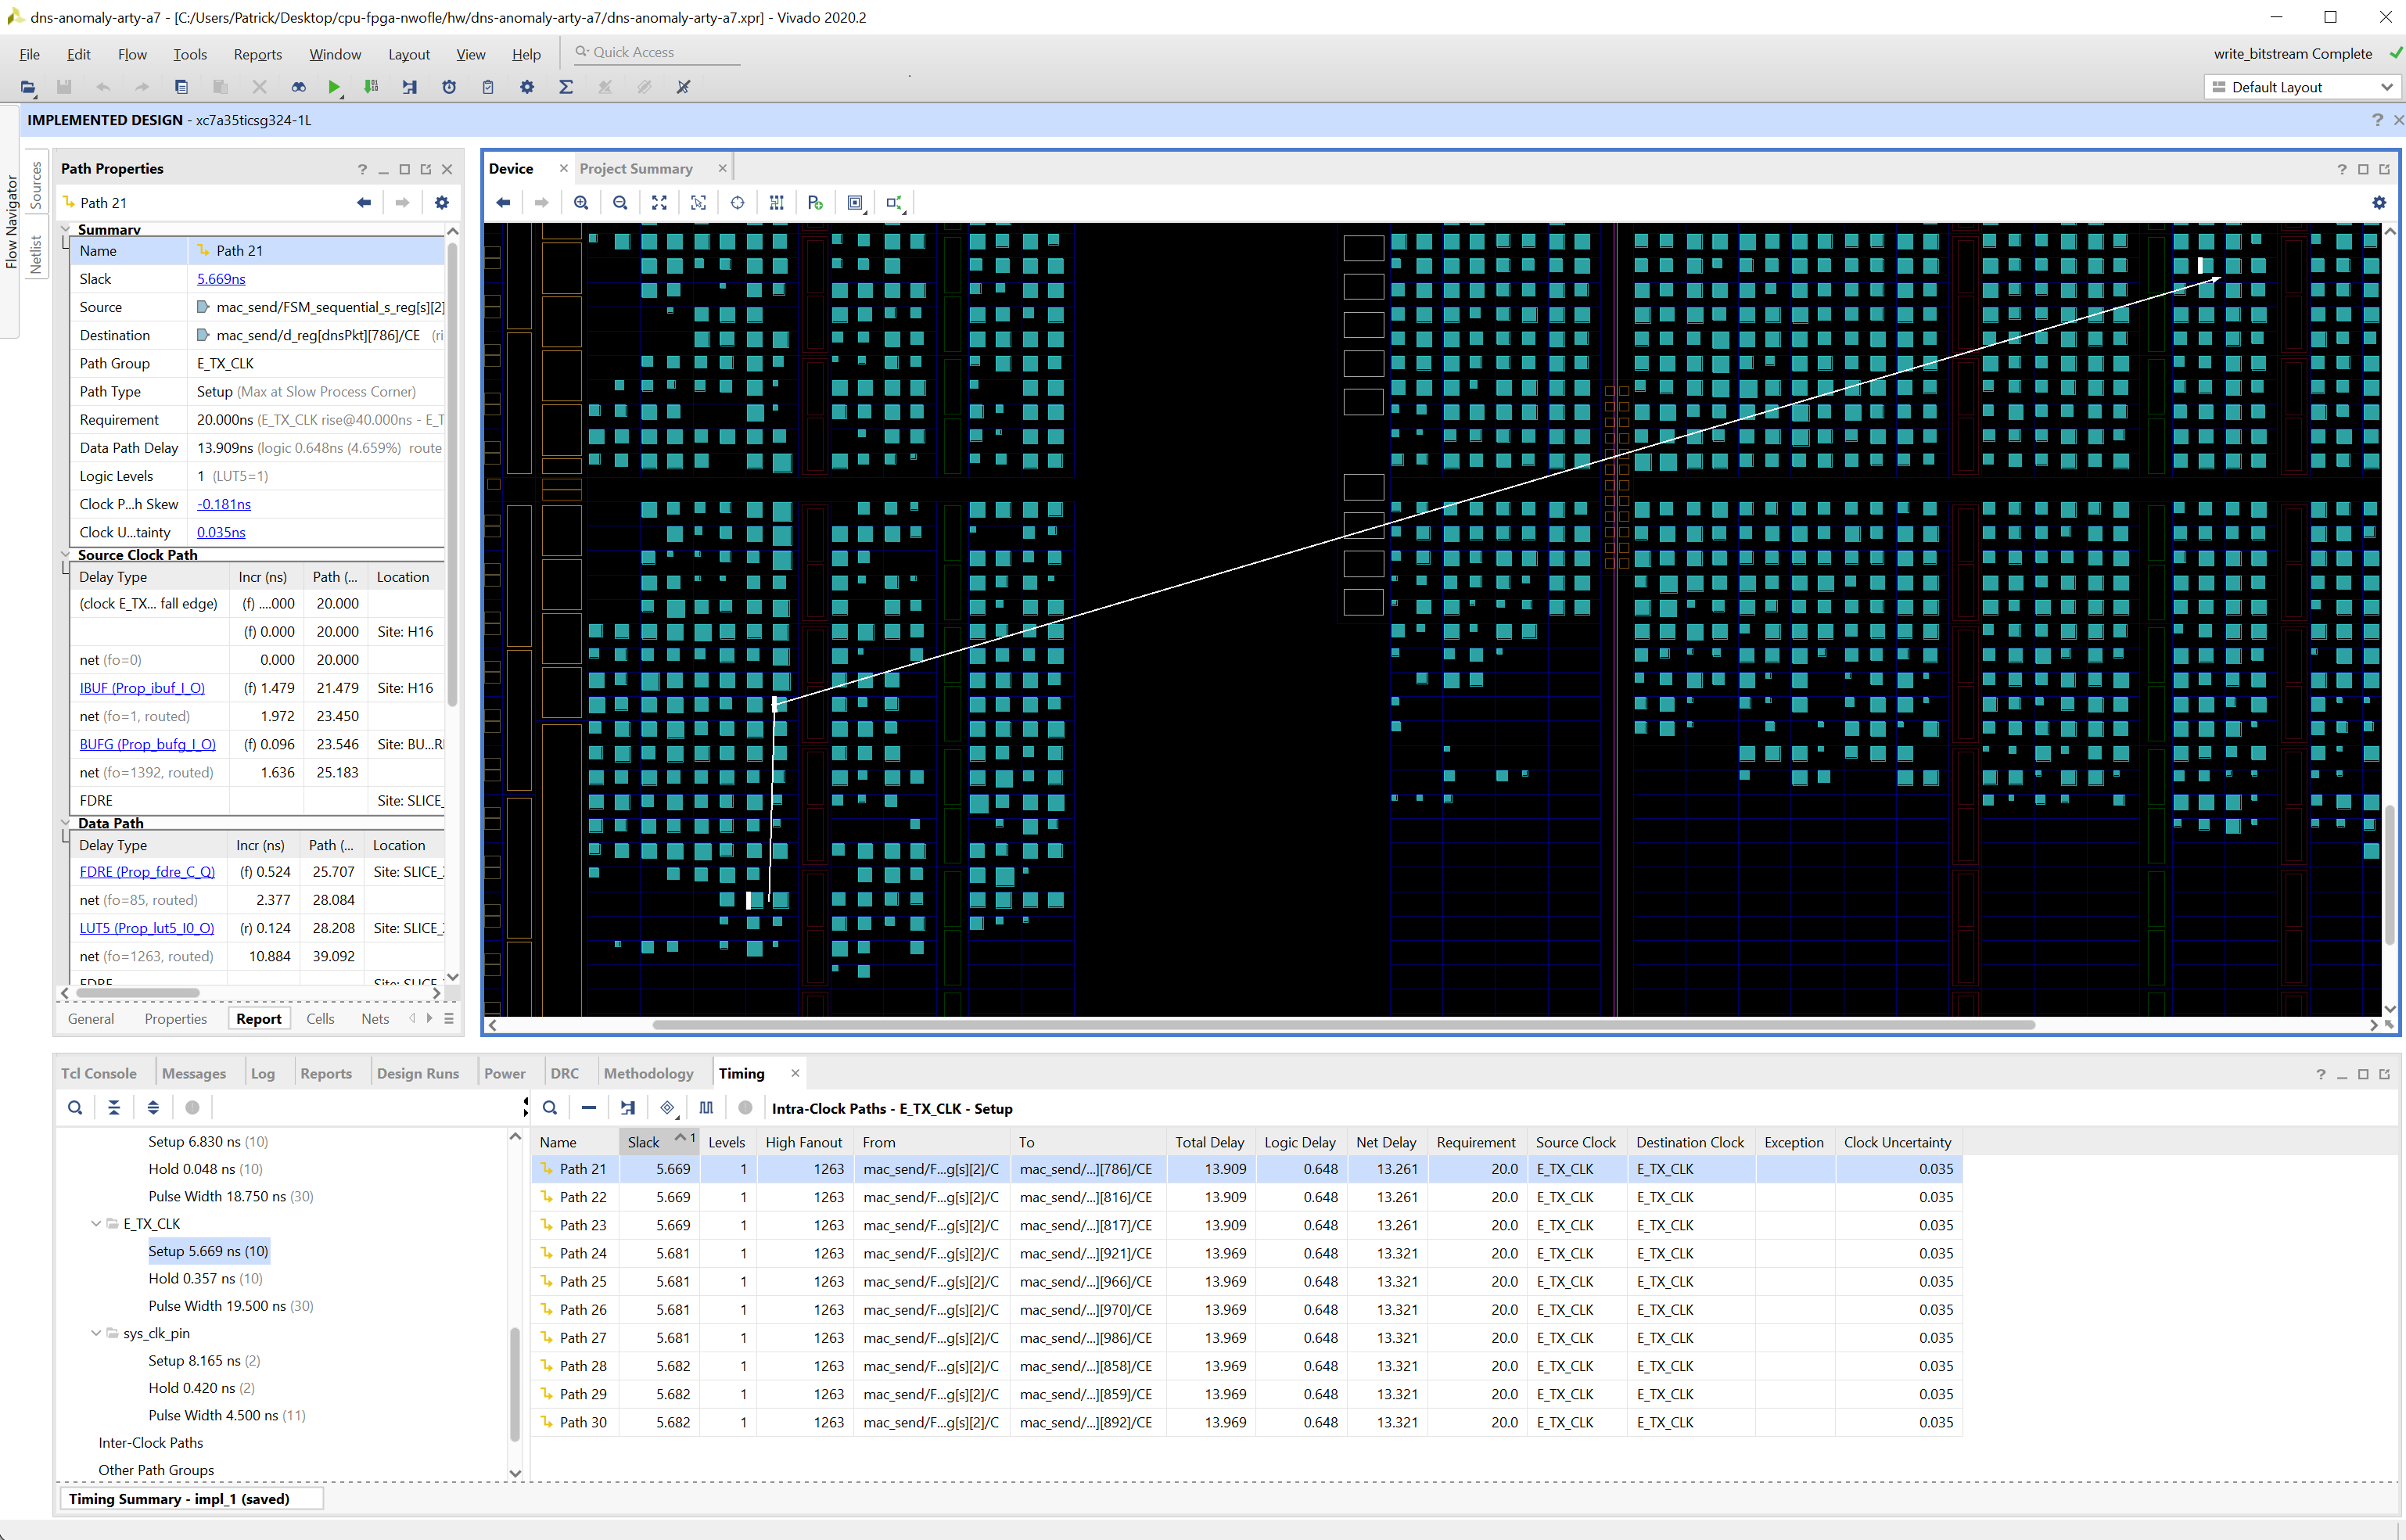
\includegraphics[width=\textwidth]{imgs/sta-in-action.png}}
  \caption{STA sample in \code{Vivado 2020.2} on a path with worst setup time of the MAC peripheral}
  \label{fig:sta-in-action}
\end{figure}

The exact nature of signal arrival can vary due to numerous (Power, Voltage, Temperature) PVT reasons. In an attempt to minimise the error caused in a complex system and ensure proper circuit operation, FPGA design tools like \code{Vivado} includes Static Timing Analysis (STA) as part of the place and route implementation process shown in Figure \ref{fig:sta-in-action}.

Typically, as the system gets increasingly complex, there is a higher chance that the design would trigger some maximum time violations. This is usually the result of having several logic paths being too deep within a clock cycle or designing a signal required to drive too many other signals throughout the circuit. When implementing the DNS payload filter, as shown in Listing \ref{lst:correct-comparison}, Section \ref{section:implementation-hardware-debugging-hdl-pitfalls-simulation-and-implementation}, all the code within the listing describes the circuit behaviour within the same clock cycle. Essentially, we are attempting to put both packet size comparison (\code{s.fpktc} to bits count) and packet content comparison (\code{rd.dnsPkt} segment to \code{f.dnsList(s.fdnsc) segment}) logic circuits between two registers, which could be too deep for this board's timing requirements. Therefore, we need to pipeline the single task into various clock cycles to reduce the logic depth. As laid out in Listing \ref{lst:pipelined-design-dns-comparison}, multiple extra states are introduced to minimise the amount of logic within the same clock cycle. Although this would surely increase the overall computation time and latency, as it now takes four times more clock cycles to process the same amount of information, we are strictly constrained by the overall chip capability regarding timing and cannot compress the logic even further.

Another example of timing constraint violation occurs when we abuse counter \code{c} on multiple occasions. As seen in a minimal example from Listing \ref{lst:signal-driving-abuse}, we are using the same counter \code{c} in all cases across the parsing states. This would give the router more difficulty when placing the registers storing \code{c} as the signals it drives are scattered around the chip. The speed of light lower bounds signal traverse time and the distance would matter quite substantially on a picosecond level. As the designer, we would need to declare multiple signal counters (i.e. \code{r.ipc} and \code{r.udpc}) for different stages to make sure the placement is more localised and alleviate the drive load on each of the counters. 

Unlike software compilers, which could make optimisations as long as the logic remains intact, the hardware synthesiser would not actively optimise the timing by allocating more registers or introducing more pipelining. Compared to software engineering, it is undoubtedly much more complex, but we do gain much more complete control over the exact steps of computation when implementing a hardware-based system.

\begin{minipage}{.45\textwidth}
\begin{lstlisting}[language=VHDL, caption=Pipelined design from Listing \ref{lst:correct-comparison}, label={lst:pipelined-design-dns-comparison}]
WHEN CmpPktCheck =>
  ...
  IF (s.fpktc >= 32) THEN
    sin.s <= CmpPktArea32;
  ELSIF (s.fpktc >= 24) THEN
    sin.s <= CmpPktArea24;
  ELSIF (s.fpktc >= 16) THEN
    sin.s <= CmpPktArea16;
  ELSIF (s.fpktc >= 8) THEN
    sin.s <= CmpPktArea8;
  ELSE
    ...
  END IF;

WHEN CmpPktArea32 =>
  IF COMPARE_32_BITS THEN
  ... ELSE ...
  END IF;

WHEN CmpPktArea24 =>
  IF COMPARE_24_BITS THEN
  ... ELSE ...
  END IF;

WHEN CmpPktArea16 =>
  IF COMPARE_16_BITS THEN
  ... ELSE ...
  END IF;

WHEN CmpPktArea8 =>
  IF COMPARE_8_BITS THEN
  ... ELSE ...
  END IF;

WHEN CmpPktDone =>
  IF (s.fpktmf = '1') THEN
    -- there's a match
  ELSIF ... THEN
    -- all check done
  ELSE
    -- increment pkt counter
  END IF;

\end{lstlisting}
\end{minipage}\hfill
\begin{minipage}{.45\textwidth}
\begin{lstlisting}[language=VHDL, caption=Minimal Example in \proglang{VHDL} of a signal driving too many other signals, label={lst:signal-driving-abuse}]
TYPE rcv_t IS RECORD
s : state_t; -- Parse State
c : NATURAL RANGE 0 TO 65535; -- Count
END RECORD;
SIGNAL r, rin : rcv_t
:= rcv_t'(
  s => Preamble,
  c => 0,
);
BEGIN
  rcv_nsl : PROCESS (E_RX_CLK)
  BEGIN
  ...
    CASE r.s IS
      WHEN Preamble =>
        IF r.c = 15 THEN 
          rin.c <= r.c ...; ELSE ...;
        END IF;        
      WHEN StartOfFrame =>
        IF r.c = 1 THEN 
          rin.c <= r.c ...; ELSE ...;
        END IF;
      WHEN EtherMACDST =>
        IF r.c = 5 THEN 
          rin.c <= r.c ...; ELSE ...;
        END IF;
      WHEN EtherMACSRC =>
        IF r.c = 5 THEN 
          rin.c <= r.c ...; ELSE ...;
        END IF;
      WHEN EtherType =>
        IF r.c = 1 THEN 
          rin.c <= r.c ...; ELSE ...;
        END IF;
      WHEN IPIHL => ... -- Uses r.c
      WHEN IPVersion => ... -- Uses r.c
      WHEN IPDSCPECN => ... -- Uses r.c
      WHEN IPLength => ... -- Uses r.c
      WHEN IPID => ... -- Uses r.c
      ...
\end{lstlisting}
\end{minipage}

\subsection{Resource Pitfalls - FPGA Placement Constraints}

As mentioned in Section \ref{section:introduction-tools-hardware}, we initially started with the Spartan 3E Starter Kit board, which was released back in 2006. The board consists of a \code{XC3S500E} core with $10,476$ logic cells \cite{xilinx-documentation-2011-core} and a SMSC \code{LAN83C185} $10/100$ Mbps Ethernet PHY chip. However, once we had implemented the MAC peripherals on the PHY interface, as specified in Section \ref{section:implementation-hardware-implementation-phy-mac-peripheral}, the LUT usage was already around $9500$ ($90\%$). Moreover, as the utilisation is very high, the placer and router face difficulties in making the design meet the timing requirements due to space limitations. To make this work, then, it would be necessary to optimise the resource usage; otherwise, the system would not work correctly, not to mention the fact that the to-be-designed core processing unit would simply be running out of logic slices. 

We identified the key issue causing the resource shortage mentioned above: using too much distributed RAM (LUTRAM) across the design instead of Block RAM (BRAM). Typically, if chunks of \code{STD\_LOGIC\_VECTOR} are declared in HDL with various types of access patterns, the synthesiser infers a distributed RAM made up of LUT. Although distributed RAMs are more flexible and faster, they are made up of logic units within the FPGA. On the other hand, implementing BRAM requires the designer to follow a given synchronous data access pattern by addresses, with the same number of bits retrieved in each clock cycle. Hence, the synthesiser could realise the designer's intent and activate the FPGA's BRAM. BRAM is usually much larger in storage capacity but lacks flexibility and can be slower than LUTRAM at times. 

\begin{figure}[h!]
  \makebox[\textwidth][c]{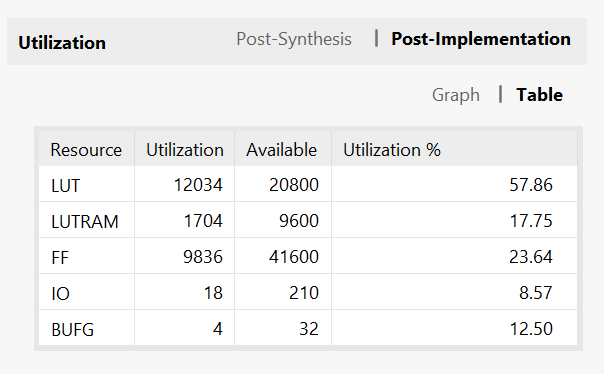
\includegraphics[width=0.56\textwidth]{imgs/utilisation-fpga.png}}
  \caption{Final Project Utilisation as reported by \code{Vivado 2020.2}}
  \label{fig:utilisation-fpga}
\end{figure}

However, as the packet array's parsing goes on, the packet array would be fragmented as different pieces of information would be required by separated components. As an experiment of using BRAMs showed, access to BRAM would be heavily congested upon packet arrival as each component gets the signal to fetch fragments of the new packet. Hence, we would also need a FIFO at the input and a dispatch unit at the output to organise all BRAM accesses. This is considered inefficient as we are using even more LUT to regulate BRAM access, and the amount used could be larger than simply using distributed RAM. Hence, we made the decision to purchase a newer board, the Digilent Arty-A735T with a \code{XC7A35T} FPGA boasting $33,280$ logic cells\cite{xilinx-documentation-artix}. As the final utilisation statistics turned out (Figure \ref{fig:utilisation-fpga}), the system would ultimately utilise $12,034 + 1,704 = 13,738$ logic units, surpassing the total amount available on the Spartan 3E Starter Kit.

\subsection{Hardware Debugging Methodologies}

As outlined in multiple sections above, debugging hardware is notoriously hard given its non-deterministic results and limitations in tools. Before we deal with any debugging in hardware, it is crucial that we make sure simulation results behaves as expected, as it at least guarantees some level of correctness in the HDL code\footnote{See Section \ref{section:validation-simulation} for more information on HDL simulation}. 

In most cases, getting it right in the simulator would not mean getting it to work in the hardware. There could be various timing errors that cannot be reflected in the STA simulation, which breaks the system. One of the most frequently used tools is the 4 LED lights on the board. As this represents 16 different states, we can put \code{LED <\null= x"6";} statements in the design to visualise the execution state. Such statements need to be placed deliberately to make sure the LEDs would actually light up and hold instead of flashing quickly, because the circuit executes on a nanosecond level.

One might ask, as a network project, we can utilise network packets to observe the internal states. This is partially possible as we can retrieve certain information (i.e. packet missing, duplicate packets) from the network behaviour. However, most NIC nowadays would offload Ethernet, IP checksums and sizes calculations. In other words, the operating system network stack would not even receive the packet if any of the payloads is incoherent with checksums or size fields. In some cases, the FPGA implementation was faulty and kept sending packets at a $10\; \mu s$ interval non-stop. These packets flooded the testing machine, spiked the CPU usage and killed \code{Wireshark} as a result. Hence, it was feasible to debug the hardware during later stages of the development, but it was simply not possible to do so when we were still developing MACs and packet constructors.

\begin{figure}[h!]
  \makebox[\textwidth][c]{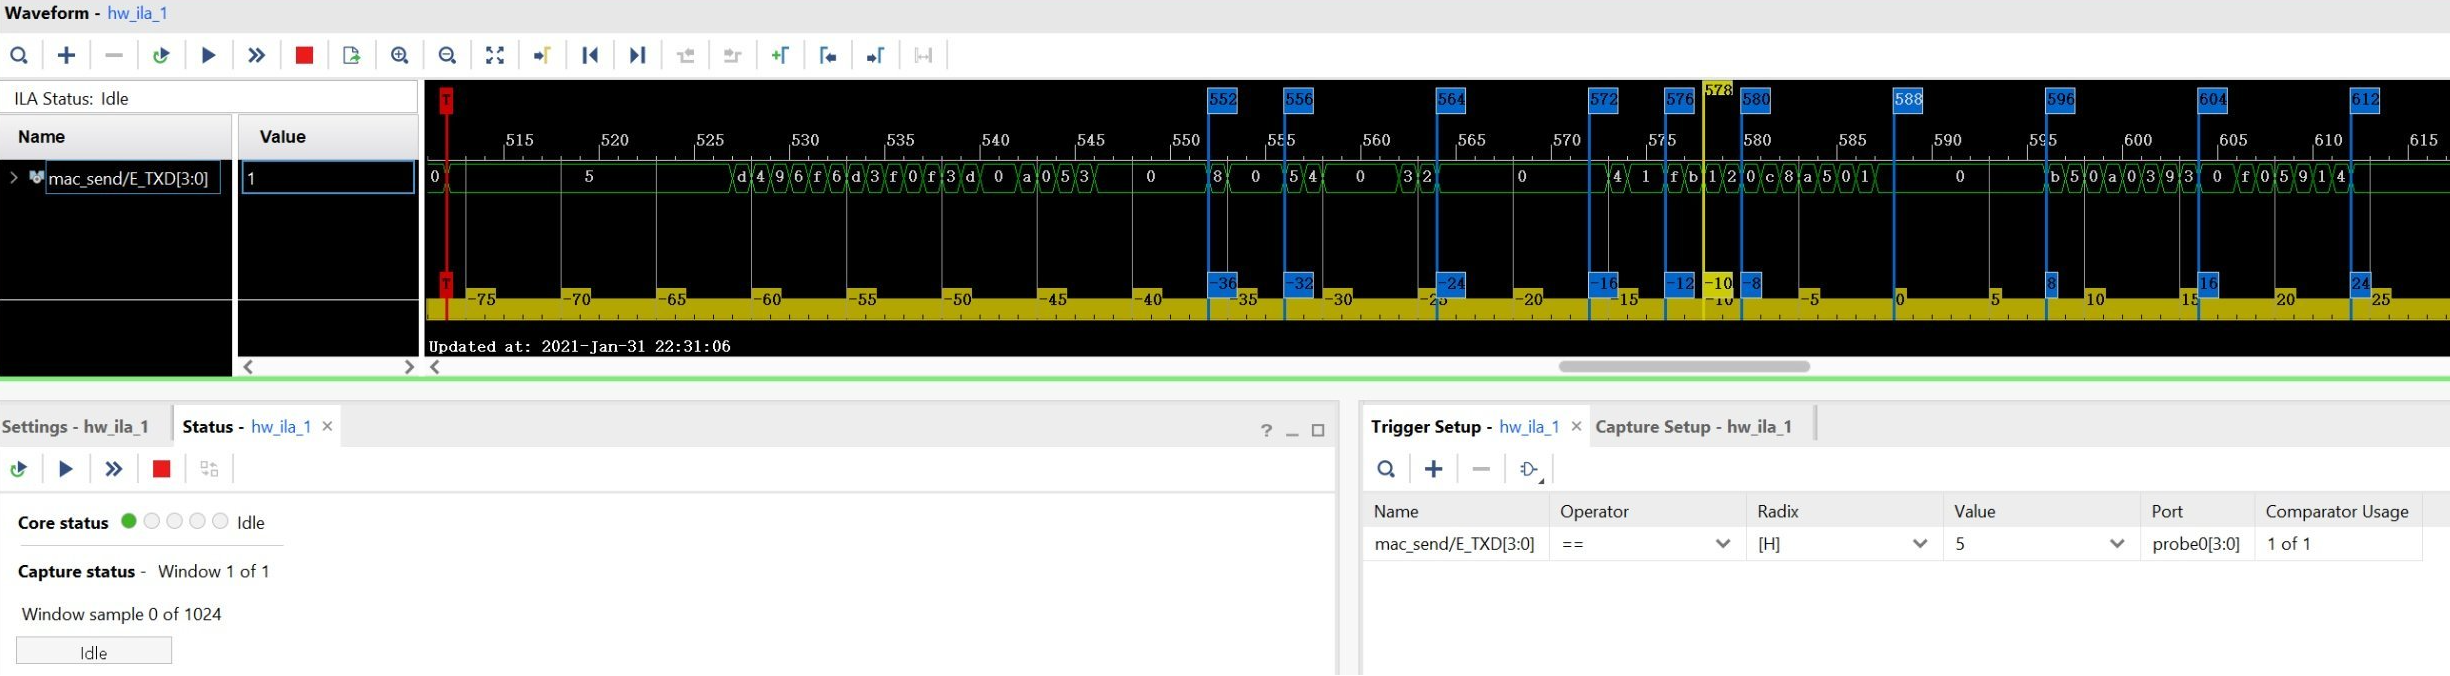
\includegraphics[width=\textwidth]{imgs/ila.png}}
  \caption{ILA debugging trigger sample with \code{Vivado 2020.2}}
  \label{fig:ila-debug-fpga}
\end{figure}

The Xilinx development environment provided a tool named ChipScope Integrated Logic Analyser (ILA) that can be synthesised into the hardware. It provides an IP core that reports to \code{Vivado} the subsequent several clock cycles (typically $1024$) of internal hardware states once triggered by a preset condition. Figure \ref{fig:ila-debug-fpga} shows an example of ILA debugging in progress. The bottom left corner shows that the ILA is triggered when \code{E\_TXD} reaches Preamble $\mathtt{0x5}$. Then, 1024 clock cycles worth of internal states on the \code{E\_TXD} signal is captured for further review. However, ILA has timing and resource limitations as in how many states to capture and how many signals can be captured simultaneously. If violated, the system will exhibit unexpected behaviour and the uploaded waveform from the FPGA will not be decodable.

\section{Software Control System}

The software system implementation can be mainly divided into three parts, namely the CLI interface (front-end), the FPGA utilities (middleware) and communication infrastructure with the FPGA (back-end).

\subsection{CLI interface}

The front-end functionalities are built based on the Edit line Library \code{libedit} that provides extensive CLI APIs. Hence, our application can have application history, auto-completion infrastructure out of the box.

\begin{lstlisting}[language=C++, caption=\code{COMMAND} structure,  label={lst:command-structure}]
typedef struct {
   const char *name;    /* User printable name of the function. */
   rl_icpfunc_t *func;  /* Function to call to do the job. */
   const char *doc;     /* Documentation for this function.  */
} COMMAND;

COMMAND commands[] = {
  { "admin", com_admin, "FPGA filter administrator utilities" },
  { "stats", com_stats, "FPGA filter stats utilities"},
  { "test", com_test, "FPGA test utilities"},
  ...
  { (char *)nullptr, (rl_icpfunc_t *)nullptr, (char *)nullptr }
};

COMMAND admin_commands[] = {
  { "show", com_admin_show, "show current / on-FPGA admin configurations [fpga/curr]" },
  { "edit", com_admin_edit, "edit current admin configurations" },
  ...
  { (char *)nullptr, (rl_icpfunc_t *)nullptr, (char *)nullptr }
};
\end{lstlisting}

When receiving an string input from the user, the parser parses the string delimited on space, and queries the function pointer table named the \code{COMMAND} struct (shown in Listing \ref{lst:command-structure}), with regards to the function to be called. Designed with the delegation pattern in mind \cite{gamma-1995}, each higher-level command queries their own table and delegates the task to a lower-level command recursively  until a final utility function is called. For example, when a user types in \code{admin show fpga}, the command look up process will be delegated to \code{execute()}, \code{com\_admin()} and \code{com\_admin\_show()} respectively. Function \code{com\_admin\_show()} would receive the stripped down parameter \code{fpga} and call the relevant middleware function to complete the task. 

\subsection{FPGA Utilities}

Functions in this layer handle the transition from FPGA messages to software understandable structures. In particular, the SipHash software implementation is included, along with bit compress and decompresses functions and bit/byte-endianness correction utilities. Several temporary states/caches are stored within this layer, including the current admin configuration in edit, waiting to be applied, the last queried FPGA status and metrics, etc. Several notable functions in this layer are:
\begin{itemize}
    \item \code{parse\_probe\_pkt} that uses bit manipulation functions to parse the bit-compressed FPGA probe response and validate its integrity.
    \item \code{write\_admin\_pkt} that writes the administration payload, compresses it into FPGA-recognisable bit format, and appends a SipHash verification MAC to the payload.
    \item \code{test\_dns\_filters}, \code{test\_reply\_filters}, and other \code{test} functions that generates random packets and validates hardware correctness.
    \item \code{print\_fpga\_stats}, \code{print\_fpga\_configurations} and other \code{print} functions that aligns and prints the messages to \code{stdout} for users to examine, see Figure \ref{fig:console-screenshot} for a CLI print example.
\end{itemize}

\begin{figure}[h!]
  \makebox[\textwidth][c]{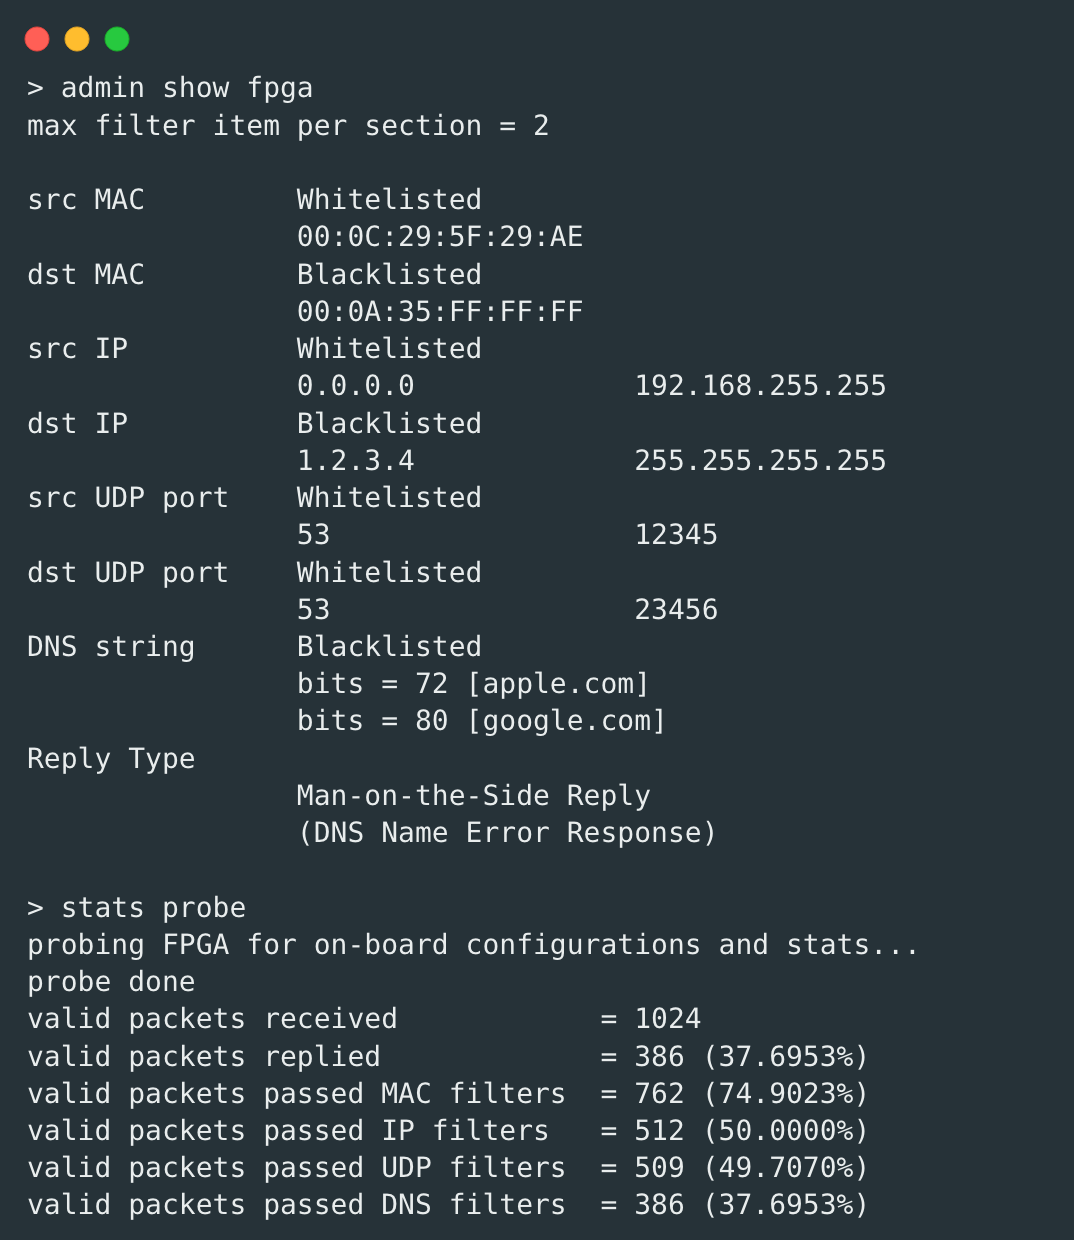
\includegraphics[width=0.56\textwidth]{imgs/console-sample.png}}
  \caption{Configuration and Metrics Captured on the FPGA shown to user}
  \label{fig:console-screenshot}
\end{figure}

\subsection{FPGA Communication Infrastructure}

In the bottom layer, two main threads handle sending and receiving packets respectively to and from the FPGA. Since sending packets is only a function call, we integrate this behaviour within the main thread. However, receiving reports and metrics from the FPGA requires constant listening that may block the main thread. Hence, we utilised another thread to do the receiving asynchronously. When the thread receives a packet on the raw socket that belongs to the FPGA and is of interest, it records the packet, calls the parser, and stores the parsed structure in the cache.

\subsection{Other software tools and utilities}

Throughout the development process, we also developed several utilities that were particularly useful. 

\begin{itemize}
    \item \code{admin\_builder}: a command-line tool that builds a desired administration packet based on command line arguments, saves and loads admin configurations to and from files. It was later integrated into the system as command \code{admin}.
    \item \code{crc32\_checker}: a command-line tool that generates/checks Ethernet CRC32 FCS from binary / text files. It was instrumental at the early stages of debugging to compare results with the hardware simulator.
    \item \code{siphash\_checker}: a command-line tool that generates/checks SipHash MAC checksum from binary / text files. It was adapted based on the software reference implementation \cite{aumasson-bernstein-2012} to validate hardware implementation.
    \item \code{pkt\_recevier/pkt\_sender}: a command-line tool that interacts with raw socket (Linux) / BPF (BSD-based systems) to send and receive packets to and from the FPGA. It takes input from command line arguments and adapts to lower-level OS accordingly. It was later integrated into the back-end of the software system.
\end{itemize}

\section{Implementation Summary}

The system's implementation realises the design into FPGA core and \proglang{C++} code in an efficient manner. With regards to the hardware implementation, we discussed in-depth its details and the difficulties faced. Overcoming these challenges requires a thorough understanding of the HDL, the hardware architecture, the FPGA timing models, the interfacing PHY ASIC and the available debugging toolsets. Meanwhile, regarding the controlling software, it was built with modularity in mind to ensure scalability and maintainability in the long run.

\chapter{Validation and Evaluation}

This chapter will be elaborating on the tests and validations designed to ensure the FPGA-based system's correctness. Also, we will be measuring the system's performance and evaluating its usability and scalability. 

\section{Simulation Testbenches}
\label{section:validation-simulation}

We first validate the HDL design's correctness by constructing test benches in \proglang{VHDL}. The testbench is comprised of several components listed below:

\begin{itemize}
    \item \code{test\_main.vhd}: The top-level test unit instantiates the \code{main} component and defines clock signals simulating the oscillators. Tests are called in the simulation main function of the unit.
    \item \code{test\_dns\_pkts.vhd}, \code{test\_srcip\_pkts.vhd} ... : These units include test cases for each hardware feature, compiled by calling infrastructural packet functions in a given sequence. 
    \item \code{test\_pkt\_infra.vhd}: This unit contains infrastructural test functions simulating fragments of packets sent to the MII interface. Basic package functions such as \code{receive\_preamble()} and \code{receive\_admin\_config()} are provided for higher level test cases.
\end{itemize}

\begin{figure}[h!]
  \makebox[\textwidth][c]{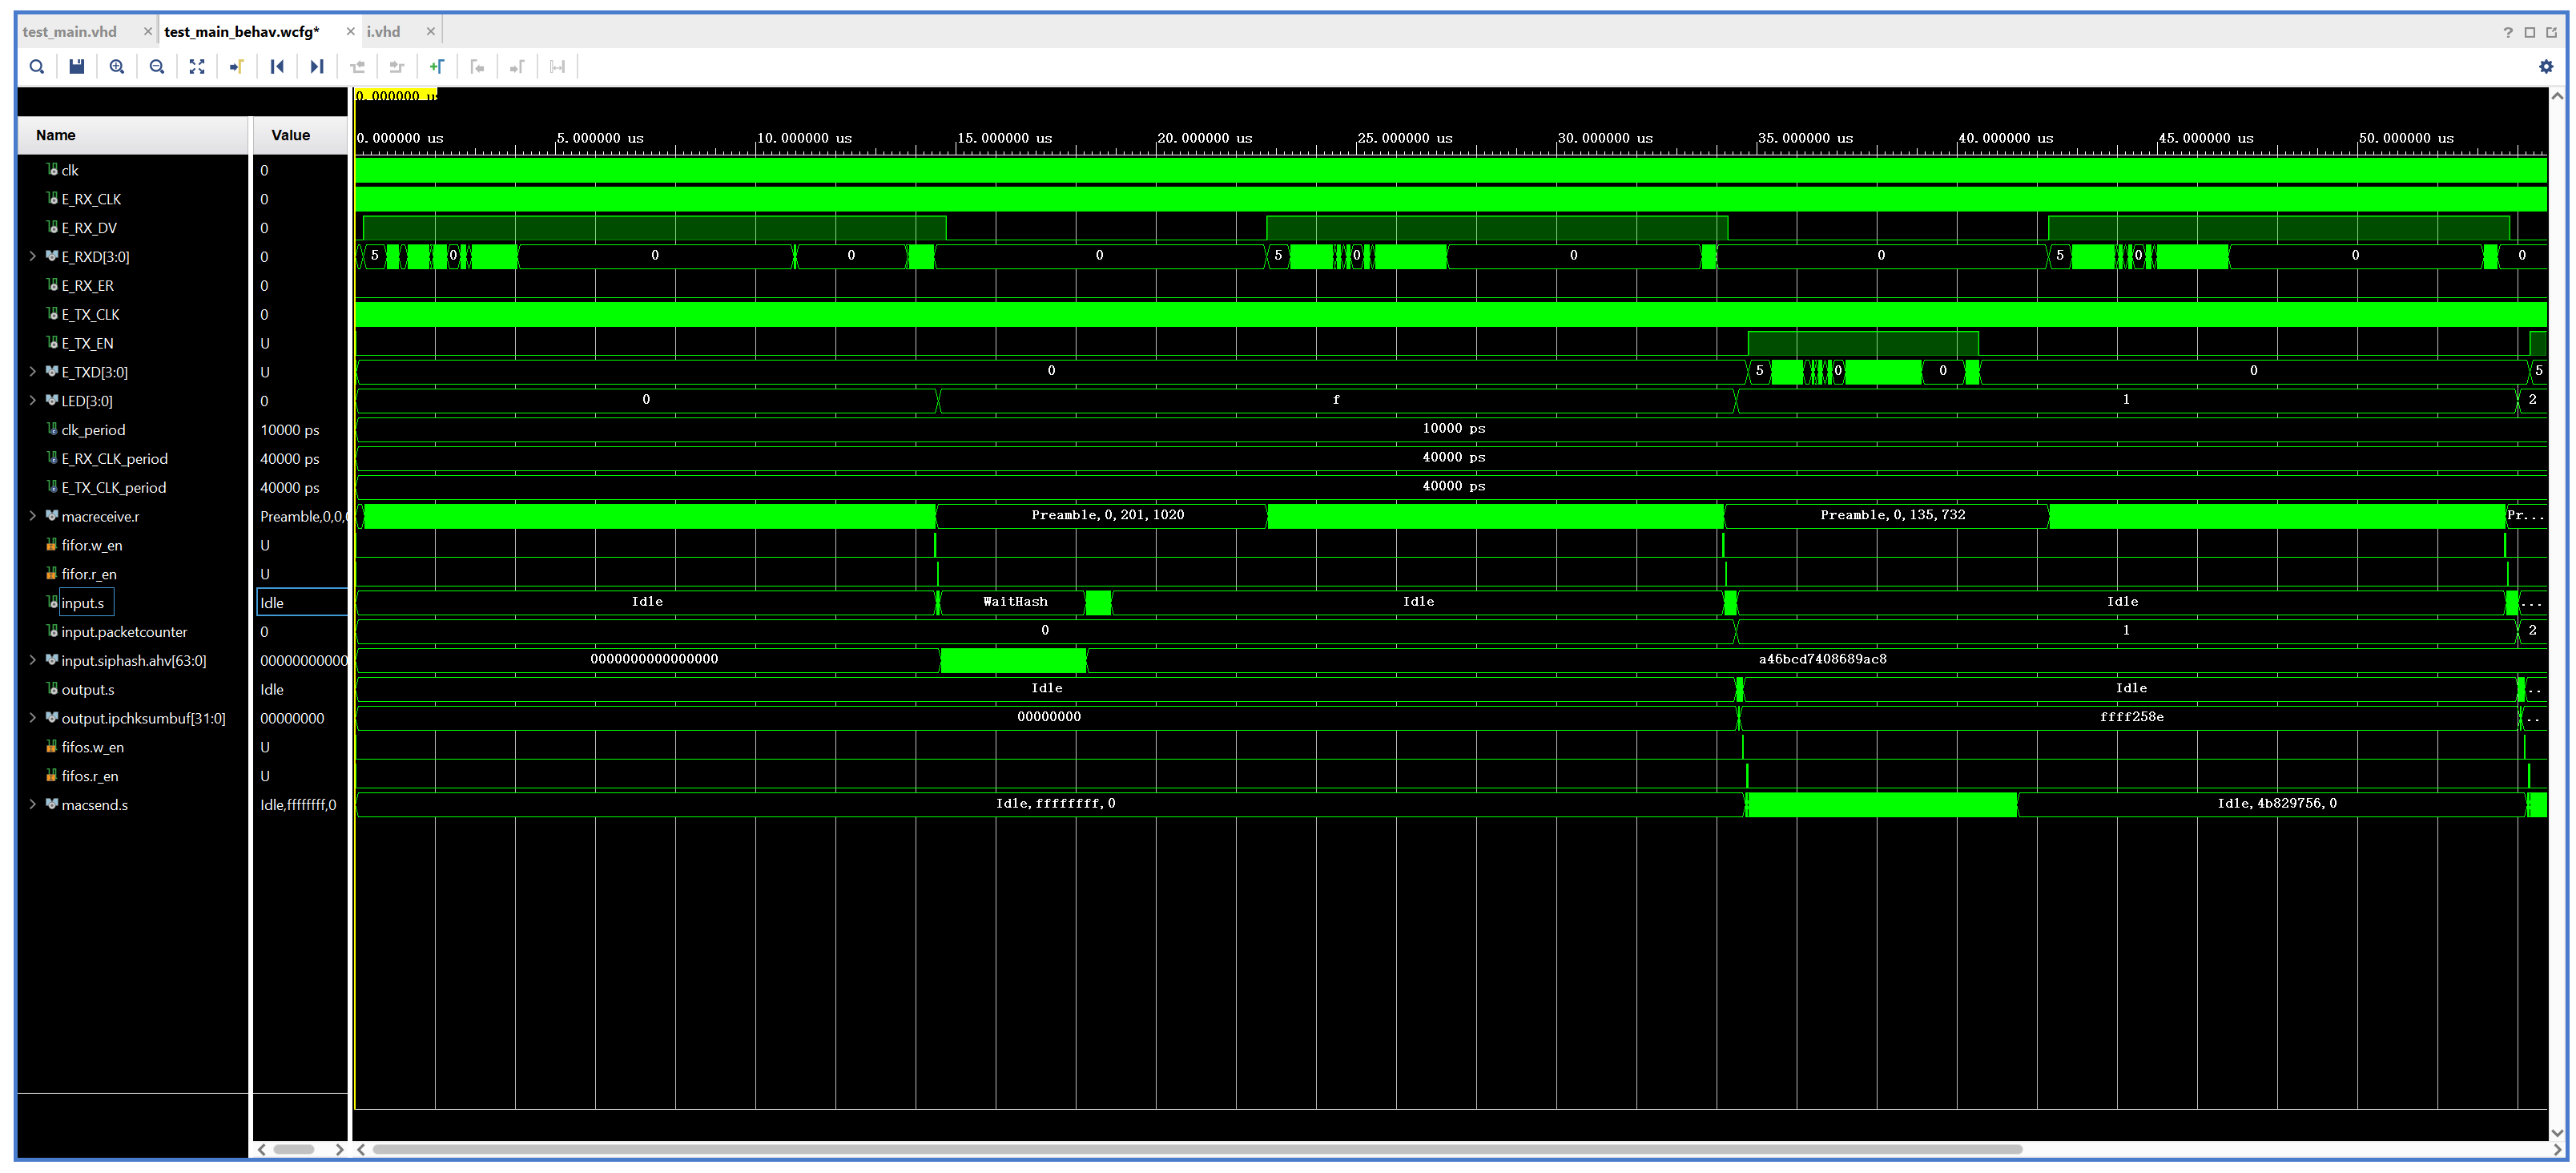
\includegraphics[width=\textwidth]{imgs/simulation.png}}
  \caption{Behavioural Simulation of the system in \code{Vivado 2020.2}}
  \label{fig:behavioural-simulation-fpga}
\end{figure}

Within the test benches' behavioural simulation, HDL object states are transparent for review, similar to single-stepping with a software debugger. Breakpoints can be set in HDL code to monitor signal states at a given instant. This step confirms the general logic correctness independent of the actual implementation. An example of behavioural testbench simulation is shown in Figure \ref{fig:behavioural-simulation-fpga}. Zooming in on the waveform would enable us to view the anticipated HDL state at each instant on a picosecond level.

After synthesis and netlist generation, we can instruct \code{Vivado} to simulate on a netlist level or even on a chip level after implementation. The simulation results can be more accurate and closer to hardware. However, we are no longer able to set breakpoints or view the HDL objects. Instead, we will be provided with hardware netlists information at each instant.

Our system has passed all simulation test cases at behavioural, netlist and chip levels, with a $100\%$ simulation coverage.

\section{Hardware Integration Testing via Software System}

Concerning the aforementioned issues in Section \ref{section:implementation-hardware-debugging}, we constantly faced regressions in functionalities upon completely unrelated changes in HDL. Hence, we developed a hardware verification utility in software to conduct integration testing so as to spot any function regression at the earliest point. The system was later integrated into the software control system as the \code{test} command. 

When testing the hardware, the system would first generate pseudo-random admin configurations with MAC/IP addresses, UDP ports and DNS domains. It was then applied to the FPGA and instantly probed and read back to validate the deployment and probe functionality. Then, the system would stress test the FPGA by flooding packets with random patterns as fast as the software is capable, validating the checkers in the FPGA. The same procedure was repeated with emphasis on different parts of the filters, operation modes, and packet constructors, each with three runs, to ensure the hardware circuit's correctness. In total, roughly 1200 packets were be communicated on the wire throughout the tests. 

\begin{figure}[H]
  \makebox[\textwidth][c]{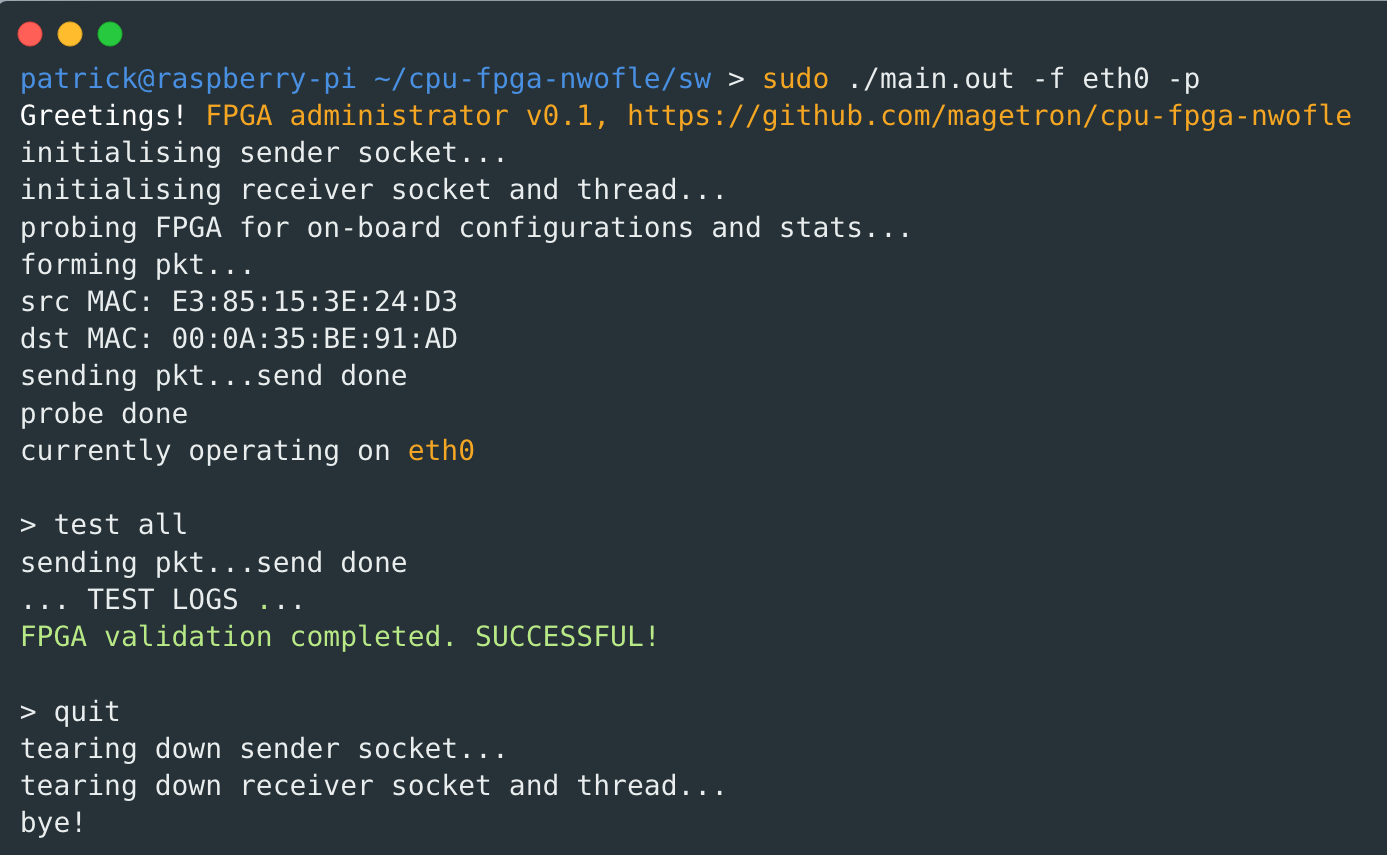
\includegraphics[width=0.72\textwidth]{imgs/test-screenshot.png}}
  \caption{Hardware validation results via the Software System}
  \label{fig:hardware-validation-results}
\end{figure}

As shown in Figure \ref{fig:hardware-validation-results}, the submission candidate version of the system passes all integration and stress tests.

\section{Evaluation}

We further evaluate the FPGA-based design and system in terms of performance, power consumption and design scalability.

\subsection{Performance}

The performance is evaluated by executing the software stress tests mentioned above with a Raspberry Pi 4i (Broadcom BCM2711 with Integrated Gigabit Ethernet Controller) and measuring the reply latency. Given the equipment limitations, we are unable to accurately measure the exact latency induced by the Raspberry Pi NIC and the signal travelling on the Ethernet cable. Hence we are estimating the extra latency according to publicly available data sheets and standards. According to IEEE 802.3 \cite{ieee802.3ethernet-2018}, the propagation delay on an standard Cat5 Ethernet cable would be around $5.30 \; ns/m$. Thus we calculate the round trip latency on the $2.5 \; m$ cable as  
$$
t_r = 2.5\; m \times 2 \times 5.30\; ns /m = 0.0265 \; \mu s
$$ 
A gigabit NIC encoding and decoding a packet for the twisted pair Cat 5 cable is estimated to take around $5 \; \mu s$ \cite{texas-instruments-dp83848x}, including system bus and Interrupt Request (IRQ) latency of $5 \; \mu s$. Hence, we estimate the total extra latency of one decode, one encode, and one interrupt to be around $15.00\; \mu s$.

Wireshark records the packet communications throughout the test cases, and we calculated the trimmed Round Trip Time (RTT) mean (95\%) as follows:
\begin{itemize}[noitemsep]
    \item Network Packets passing all checkers: $27.238\; \mu s$
    \item Spoofed DNS Reply Packets: $28.753\; \mu s$
    \item Probe Packets: $34.679\; \mu s$
\end{itemize}
See Table \ref{table:performance-test} for RTT measurements of each test case.

\begin{table}[h!]
\begin{tabular}{ll|ll|ll|ll}
\hline
testcase  & avg ($\mu s$) & testcase & avg ($\mu s$) & testcase   & avg ($\mu s$) & testcase  & avg ($\mu s$) \\ \hline
srcmac-b0 & 32.276   & srcip-b0 & 31.942   & srcport-b0 & 39.743   & dns-b0      & 24.766   \\
srcmac-b1 & 29.612   & srcip-b1 & 29.412   & srcport-b1 & 36.372   & dns-b1      & 33.065   \\
srcmac-b2 & 29.466   & srcip-b2 & 22.334   & srcport-b2 & 26.45    & dns-b2      & 27.856   \\
srcmac-w1 & 45.432   & srcip-w1 & 23.285   & srcport-w1 & 34.242   & dns-w1      & 18.767   \\
srcmac-w2 & 27.282   & srcip-w2 & 17.747   & srcport-w2 & 17.174   & dns-w2      & 18.876   \\
dstmac-b0 & 15.761   & dstip-b0 & 31.013   & dstport-b0 & 15.83    & spoof-reply & 28.753   \\
dstmac-b1 & 23.267   & dstip-b1 & 36.306   & dstport-b1 & 29.067   & probe       & 34.679   \\
dstmac-b2 & 20.942   & dstip-b2 & 16.31    & dstport-b2 & 30.15    &             &          \\
dstmac-w1 & 22.123   & dstip-w1 & 17.205   & dstport-w1 & 17.565   &             &          \\
dstmac-w2 & 18.568   & dstip-w2 & 52.721   & dstport-w2 & 40.405   &             &          \\ \hline
\end{tabular}
\caption{RTT measures of all test cases on Raspberry Pi 4B}
\label{table:performance-test}
\end{table}
Therefore, we estimate the processing latency of the FPGA as:
\begin{itemize}[noitemsep]
    \item Network Packets passing all checkers: $27.238\; \mu s - 15\; \mu s = 12.238\; \mu s$
    \item Spoofed DNS Reply Packets: $28.753\; \mu s - 15\; \mu s = 13.753\; \mu s$
    \item Probe Packets: $34.679\; \mu - 15\; \mu s = 19.679\; \mu s$
\end{itemize}
If we count in the PHY encoding / decoding time taken on the FPGA board, we estimate the processing latency of the FPGA design as 
\begin{itemize}[noitemsep]
    \item Network Packets passing all checkers: $12.238\; \mu s - 10\; \mu s= 2238\; ns$
    \item Spoofed DNS Reply Packets: $13.753\; \mu s - 10\; \mu s = 3753\; ns$
    \item Probe Packets: $19.679\; \mu - 10\; \mu s = 9679\; ns$
\end{itemize}

We are relatively confident with our approximations, as the experiment results are mainly coherent with the estimates we made during implementation in Section \ref{section:implementation-hardware-implementation}. For a low-end FPGA board at the cost of just $£96$, the network processing speed and capability it brings is quite impressive. Comparatively, the fastest DNS server powered by Unikernel Mirage OS, running on a Dell PowerEdge R710 Server with 2 Xeon E5530 processors, costing around $\$700$, has a processing latency of around $500\; \mu s$, regardless of the latency on wire \cite{briggs-2014, madhavapeddy-2013}. Thus, our solution's performance per $£/\$$ far outweighs any known DNS processors. As we have measured, a typical DNS query to a Cloudflare DNS server through the Internet takes roughly $40\;ms - 60\;ms$. Thus, we can observe that the main latency in a DNS transaction actually lies in the transmission time through the wires, which is inevitable. Hence, it is safe to say that the extra latency overhead of less than $30\; \mu s$ introduced by the system is minimal and almost negligible.

On a side note, with regards to the FPGA system also aimed at detecting malicious DNS traffic built by Brennon et al.\cite{thomas-2011}, we were unable to retrieve its performance or latency data, hence there is no comparison to this in this section.

\subsection{Power}

\begin{figure}[h!]
  \makebox[\textwidth][c]{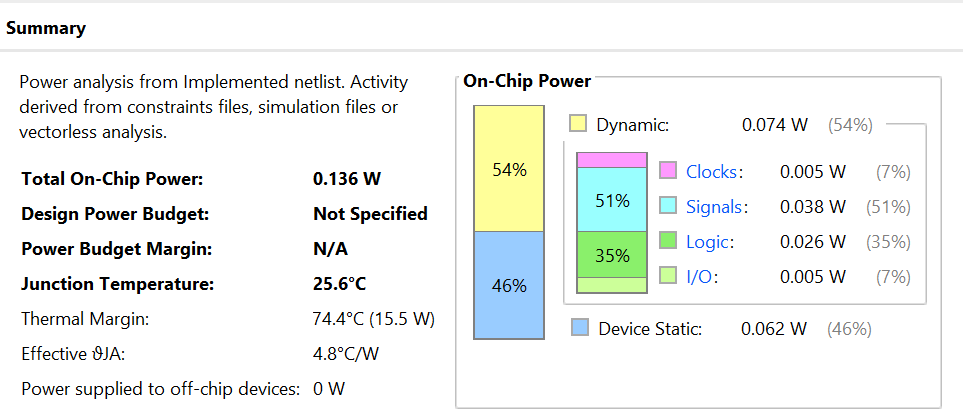
\includegraphics[width=0.8\textwidth]{imgs/power-consumption.png}}
  \caption{Power Consumption Analysis of the system in\code{Vivado 2020.2}}
  \label{fig:power-consumption-analysis}
\end{figure}

Figure \ref{fig:power-consumption-analysis} shows the power consumption analysis of the FPGA. The system is estimated to consume $0.062\;W - 0.136\;W$ depending on the working payload at a core frequency of $50$ MHz and a PHY frequency of $25$ MHz. By comparison, a much-slower software firewall \code{firewalld} on a Raspberry Pi 4B would consume around $2.7 \; W$, while an enterprise software-based firewall server would consume more than $150 \; W$ of power to achieve similar speed. Hence, for the packet processing capability it offers, the power efficiency gain on the FPGA is also quite notable.

\subsection{Design Scalability}

The HDL design and hardware implementation are scalable in multiple ways:

\begin{itemize}
    \item Filter Item Limit: Due to distributed RAM and timing constraints, we limited each type of filter to 2 items maximum. However, we tested in simulation that the HDL code is be extensible by simply changing the constant \code{filter\_depth}.
    \item Link Speed: Due to board PHY hardware constraints, we are only able to establish a 100 Mbps Ethernet link. Nonetheless, the design can scale to \code{RGMII} interface with minimal changes and support Gigabit Ethernet link speed.
    \item Clock Frequency: Due to board placement constraints, we can only set the clock speed to $50$ MHz. With a higher-end FPGA core, the clock frequency can be further increased to $200$ MHz, as tested through the simulator.
    \item Processing Bandwidth: Although a single FPGA unit is limited by the link speed of $100$ Mbps (roughly $83000$ DNS packets per second), we can increment the number of FPGAs executing in parallel to increase the packet processing capability linearly since the FPGA core can processes packets at full link speed.
\end{itemize}

\section{Validation and Evaluation Summary}

In this chapter, we discussed in depth our test methodologies in preventing regressions and validating the correctness of the FPGA-based system. From the evaluation results, we are confident that our FPGA-based solution is capable of achieving state-of-the-art packet processing speed and minimal latency while keeping its power usage ultra-low at the same time. Considering its cost, our solution provides an unparalleled price-to-performance ratio even when compared to the latest software solutions. Moreover, the design is proven through chip-level simulations to be adaptable on larger-scale hardware platforms with faster Ethernet link speeds and higher clock frequencies.

\chapter{Conclusions and Future Work}

This chapter provides a conclusive review of the project and lays out future work that can potentially be undertaken with more time and a higher budget.

\section{Future Work}

As a final year student project during COVID-19, we were constrained by a strict budget on the FPGA boards and the lack of access to network test equipment. The main hardware component, Digilent Arty-A7 35T is a low-end starter board that costs only $£96$, with a limited number of logic slices and suboptimal semiconductors. Therefore, the design is fairly limited in complexity and operation frequency, which is crucial to the system's performance and usability. Given more budget and time, the design can be improved in areas including:

\begin{itemize}
    \item Eliminating packet segment limit of $128$ bytes. We can take a streamlined approach when communicating with the PHY peripherals. FIFOs can be implemented to store larger packet payload in segments.
    \item Achieving lower latency, higher clock frequency and greater filter depth. Network processing low-latency FPGAs are mostly PCI-E boards with multiple 10 Gigabit Ethernet links, costing more than $\$6000$ \cite{netfpga-sume-digilent}. This would substantially improve the design's usability and latency with more logic slices, better timing requirements, faster PHY connection speeds, and much higher clock frequency.
    \item Conducting more accurate performance measurements. Due to COVID-19, we lacked access to computing equipment to stress test the FPGA to its limit (Raspberry Pi 4B is not sufficient) and measure the accurate latency at each stage of the packet transaction process.
    \item Handling complex string algorithms through an ARM softcore on the higher-end Xilinx Zynq FPGA board \cite{zynq-7000-xilinx}. We are currently doing DNS domain checking with the naive string comparison algorithm in pure hardware logic. We can potentially utilise the software processor to handle such task with a more complex and efficient algorithm such as a Trie or a Hashmap.
    \item Implementing stateful administrator packet authentications to mitigate malicious replay attacks. The system in its current state is vulnerable to man-in-the-middle packet replay attacks targetting the FPGA. We can mitigate this by enforcing state counters during admin packet transactions.
\end{itemize}

\section{Conclusions}
In this project, we have designed, implemented and evaluated an innovative FPGA-based system that detects and mitigates DNS flood and DNS exfiltration attacks at scale in real-time. We managed to undertake the challenges presented in hardware and high-speed network peripheral development during the process and gained a more rigorous understanding of the FPGA architecture and electrical timing models.

As the first item of the deliverable, we showed that our FPGA-based system is capable of detecting and mitigating DNS exfiltration and flood attacks. The network administrator would be able to tune the FPGA configurations so as to adapt to various attacking scenarios quickly. Most notably, the FPGA processor incorporates two operations modes, namely Man-on-the-Side DNS spoof mode and Man-in-the-Middle Payload filter mode, to detect and mitigate DNS exfiltration and DNS flood attacks, respectively. The implemented hardware has been thoroughly tested through simulation and integration tests to ensure its correctness.

Moreover, we also illustrated the performance-to-power and performance-to-cost efficiency of the proposed hardware system. The latency tests and power analysis shows that a budget FPGA (Digilent Arty-A7 35T costing $£96$) can perform the aforementioned network tasks and operations extremely quickly (minimal RTT latency of only $12\; \mu s$, packet process latency of $2500\; ns$), and with ultra-low power consumption (maximum power consumption of only $0.136\; W$). 

Additionally, our hardware solution comes with CLI software that enables network administrators to quickly apply new configurations, block/allow lists, and instantaneously retrieve FPGA metrics and status. The reconfigurability in hardware also allows higher-level algorithms to analyse the traffic and update settings simultaneously to the FPGA so as to cope with more complex attacking scenarios.

Lastly, our scalability analysis demonstrated our HDL design considerations that make it future-proof when adapting to larger boards with higher-end FPGA cores. As the simulator suggests, our hardware layout would be able to adapt to $1$ Gbps link speed, higher filter depth and $200$ MHz clock frequency in more advanced implementations.

In conclusion, we have built a novel FPGA-based system that detects and blocks malicious DNS transactions in real-time. This system is significantly more performant and cost-efficient than existing solutions against deceitful attacks that rely on the enormous amount of legitimate DNS traffic, such as DNS data exfiltration and DNS flood attacks. Moreover, our solution is unique in its scalability across networks of different sizes, its adaptability to various types of DNS-based attacks, and its ability to mitigate these threats simultaneously. This project further illustrates a massive research potential in utilising hardware to monitor large scale networks and block potential attacks on the spot in the long run.

\addcontentsline{toc}{chapter}{References}
\printbibliography[title=References]

\appendix

\chapter{Project Demo}

The project's demo video is available at: \url{https://www.youtube.com/watch?v=JdgHUCco5vk}. This video may be copied and distributed under the Creative Commons – Attribution 4.0 International License. A copy of the license can be obtained at \url{https://creativecommons.org/licenses/by/4.0/legalcode}.

\chapter{Code Repository}

The complete project, including \proglang{VHDL} source code for hardware, and \proglang{C/C++} source code for software, is open sourced at  \url{https://github.com/magetron/fpga-dns-adtm}, under Apache License 2.0. A copy of the license can be obtained at \url{https://www.apache.org/licenses/LICENSE-2.0}.

This document and the \TeX {} source code of this document shall be shared under Creative Commons – Attribution 4.0 International License. A copy of the license can be obtained at \url{https://creativecommons.org/licenses/by/4.0/legalcode}.

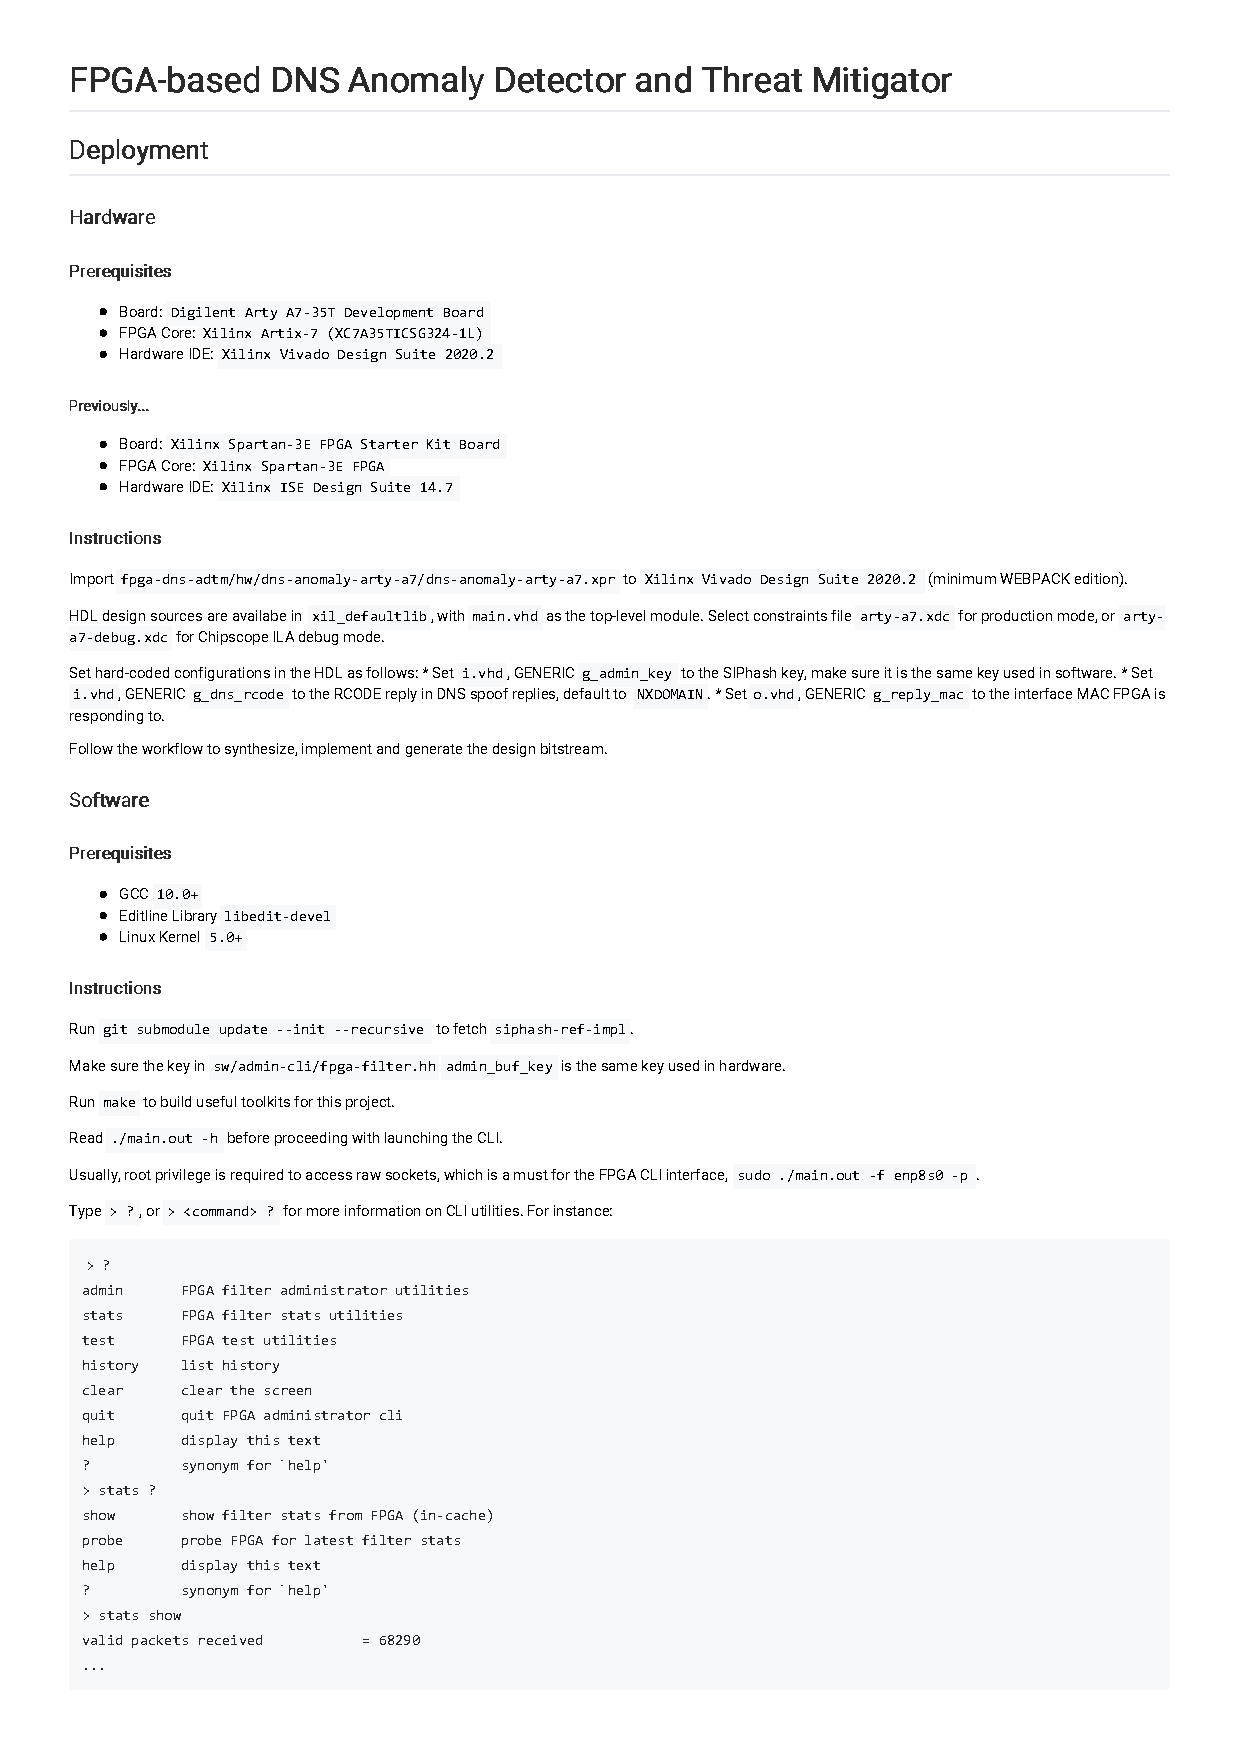
\includepdf[pages=-,addtotoc={1,chapter,1,Project Manual,pdf:project-manual}]{contents/GitHub-README.pdf}
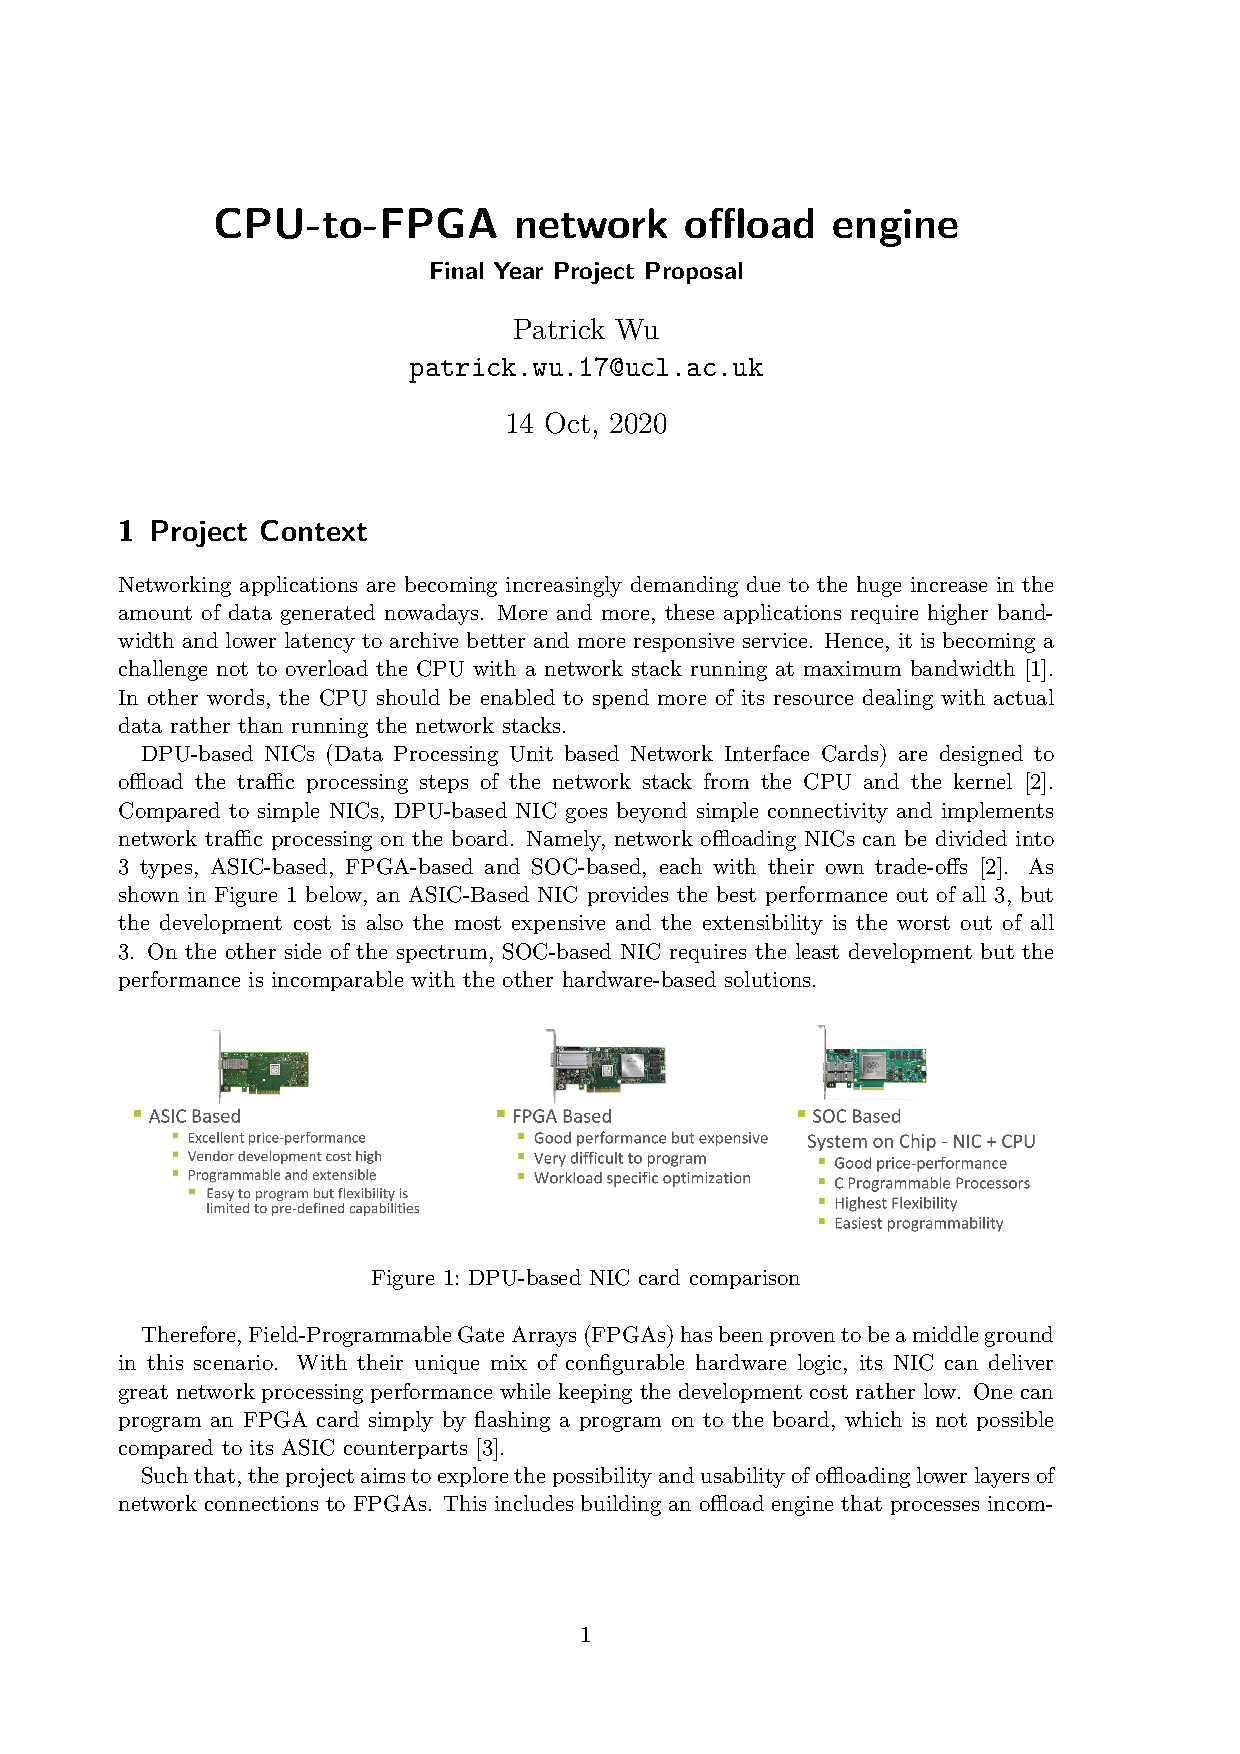
\includepdf[pages=-,addtotoc={1,chapter,1,Project Proposal,pdf:proposal}]{contents/appedix-proposal.pdf}

\end{document}